%%
%% CombinationLock GroupLab (c) 2022-24 Christopher A. Bohn
%%
%% Licensed under the Apache License, Version 2.0 (the "License");
%% you may not use this file except in compliance with the License.
%% You may obtain a copy of the License at
%%     http://www.apache.org/licenses/LICENSE-2.0
%% Unless required by applicable law or agreed to in writing, software
%% distributed under the License is distributed on an "AS IS" BASIS,
%% WITHOUT WARRANTIES OR CONDITIONS OF ANY KIND, either express or implied.
%% See the License for the specific language governing permissions and
%% limitations under the License.
%%

%%
%% (c) 2021 Christopher A. Bohn
%%

\documentclass[12pt]{article}

\usepackage{fullpage}
\usepackage{fancyhdr}
\usepackage[procnames]{listings}
\usepackage{hyperref}
\usepackage{textcomp}
\usepackage{bold-extra}
\usepackage[dvipsnames]{xcolor}
\usepackage{etoolbox}


% Customize the semester (or quarter) and the course number

\newcommand{\courseterm}{Spring 2022}
\newcommand{\coursenumber}{CSCE 231}

% Customize how a typical lab will be managed;
% you can always use \renewcommand for one-offs

\newcommand{\runtimeenvironment}{your account on the \textit{csce.unl.edu} Linux server}
\newcommand{\filesource}{Canvas or {\footnotesize$\sim$}cse231 on \textit{csce.unl.edu}}
\newcommand{\filesubmission}{Canvas}

% These are placeholder commands and will be renewed in each lab

\newcommand{\labnumber}{}
\newcommand{\labname}{Lab \labnumber\ Assignment}
\newcommand{\shortlabname}{}
\newcommand{\duedate}{}

% Individual or team effort

\newcommand{\individualeffort}{This is an individual-effort project. You may discuss concepts and syntax with other students, but you may discuss solutions only with the professor and the TAs. Sharing code with or copying code from another student or the internet is prohibited.}
\newcommand{\teameffort}{This is a team-effort project. You may discuss concepts and syntax with other students, but you may discuss solutions only with your assigned partner(s), the professor, and the TAs. Sharing code with or copying code from a student who is not on your team, or from the internet, is prohibited.}
\newcommand{\freecollaboration}{In addition to the professor and the TAs, you may freely seek help on this assignment from other students.}
\newcommand{\collaborationrules}{}

% Do you care about software engineering?

\providebool{allowspaghetticode}

\setbool{allowspaghetticode}{false}

\newcommand{\softwareengineeringfrontmatter}{
    \ifboolexpe{not bool{allowspaghetticode}}{
        \section*{No Spaghetti Code Allowed}
        In the interest of keeping your code readable, you may \textit{not} use
        any \lstinline{goto} statements, nor may you use any \lstinline{break}
        statements to exit from a loop, nor may you have any functions
        \lstinline{return} from within a loop.
    }{}
}

\newcommand{\spaghetticodepenalties}[1]{
    \ifboolexpe{not bool{allowspaghetticode}}{
        \penaltyitem{1}{for each \lstinline{goto} statement, \lstinline{break}
            statement used to exit from a loop, or \lstinline{return} statement
            that occurs within a loop.}
    }{}
}

% You shouldn't need to customize these,
% but you can if you like

\lstset{language=C, tabsize=4, upquote=true, basicstyle=\ttfamily}
\newcommand{\function}[1]{\textbf{\lstinline{#1}}}
\setlength{\headsep}{0.7cm}
\hypersetup{colorlinks=true}

\newcommand{\startdocument}{
    \pagestyle{fancy}
    \fancyhf{}
    \lhead{\coursenumber}
    \chead{\ Lab \labnumber: \labname}
    \rhead{\courseterm}
    \cfoot{\shortlabname-\thepage}

	\begin{document}
	\title{\ Lab \labnumber}
	\author{\labname}
	\date{Due: \duedate}
	\maketitle

    \textit{\collaborationrules}
}

\newcommand{\rubricitem}[2]{\item[\underline{\hspace{1cm}} +#1] #2}
\newcommand{\bonusitem}[2]{\item[\underline{\hspace{1cm}} Bonus +#1] #2}
\newcommand{\penaltyitem}[2]{\item[\underline{\hspace{1cm}} -#1] #2}

%%
%% labs/common/semester.tex
%% (c) 2021-22 Christopher A. Bohn
%%
%% Licensed under the Apache License, Version 2.0 (the "License");
%% you may not use this file except in compliance with the License.
%% You may obtain a copy of the License at
%%     http://www.apache.org/licenses/LICENSE-2.0
%% Unless required by applicable law or agreed to in writing, software
%% distributed under the License is distributed on an "AS IS" BASIS,
%% WITHOUT WARRANTIES OR CONDITIONS OF ANY KIND, either express or implied.
%% See the License for the specific language governing permissions and
%% limitations under the License.
%%


% Customize the semester (or quarter) and the course number

\newcommand{\courseterm}{Fall 2022}
\newcommand{\coursenumber}{CSCE 231}

% Customize how a typical lab will be managed;
% you can always use \renewcommand for one-offs

\newcommand{\runtimeenvironment}{your account on the \textit{csce.unl.edu} Linux server}
\newcommand{\filesource}{Canvas or {\footnotesize$\sim$}cse231 on \textit{csce.unl.edu}}
\newcommand{\filesubmission}{Canvas}

% Customize for the I/O lab hardware

\newcommand{\developmentboard}{Arduino Nano}
%\newcommand{\serialprotocol}{SPI}
\newcommand{\serialprotocol}{I2C}
%\newcommand{\displaymodule}{MAX7219digits}
%\newcommand{\displaymodule}{MAX7219matrix}
\newcommand{\displaymodule}{LCD1602}

\setbool{usedisplayfont}{true}

\newcommand{\obtaininghardware}{
    The EE Shop has prepared ``class kits'' for CSCE 231; your class kit costs \$30.
    The EE Shop is located at 122 Scott Engineering Center and is open M-F 7am-4pm. You do not need an appointment.
    You may pay at the window with cash, with a personal check, or with your NCard.
    The EE shop does \textit{not} accept credit cards.
}

% Update to reflect the CS2 course(s) at your institute

\newcommand{\cstwo}{CSCE~156, RAIK~184H, or SOFT~161}

% Do you care about software engineering?

\setbool{allowspaghetticode}{false}

% Which assignments are you using this semester, and when are they due?

\newcommand{\pokerlabnumber}{1}
\newcommand{\pokerlabcollaboration}{
    Sections~\ref{sec:connecting}, \ref{sec:terminology}, \ref{sec:gettingstarted}, \ref{subsec:typesofpokerhands}, and~\ref{subsec:studythecode}: \freecollaboration
    Sections~\ref{sec:completingcard} and~\ref{subsec:completepoker}: \individualeffort
}
\newcommand{\pokerlabdue}{Week of August 29, before the start of your lab section}

\newcommand{\keyboardlabnumber}{2}
\newcommand{\keyboardlabcollaboration}{\individualeffort}
\newcommand{\keyboardlabdue}{Week of January 31, before the start of your lab section}

\newcommand{\pointerlabnumber}{3}
\newcommand{\pointerlabcollaboration}{\individualeffort}
\newcommand{\pointerlabdue}{Week of February 7, before the start of your lab section}

\newcommand{\integerlabnumber}{4}
\newcommand{\integerlabcollaboration}{\individualeffort}
\newcommand{\integerlabdue}{Week of February 14, before the start of your lab section}

\newcommand{\floatlabnumber}{5}
\newcommand{\floatlabcollaboration}{\individualeffort}
\newcommand{\floatlabdue}{soon}

\newcommand{\addressinglabnumber}{6}
\newcommand{\addressinglabcollaboration}{\individualeffort}
\newcommand{\addressinglabdue}{Week of February 28, before the start of your lab section}

%bomblab was 7
%attacklab was 8

\newcommand{\pollinglabnumber}{9}
\newcommand{\pollinglabcollaboration}{\individualeffort}
\newcommand{\pollinglabdue}{Week of April 11, before the start of your lab section}
\newcommand{\pollinglabenvironment}{your \developmentboard-based class hardware kit}

\newcommand{\ioprelabnumber}{\pollinglabnumber-prelab}
\newcommand{\ioprelabcollaboration}{\freecollaboration}
\newcommand{\ioprelabdue}{Before the start of your lab section on April 5 or 6}

\newcommand{\interruptlabnumber}{10}
\newcommand{\interruptlabcollaboration}{\individualeffort}
\newcommand{\interruptlabdue}{Week of April 18, before the start of your lab section}
\newcommand{\interruptlabenvironment}{your \developmentboard-based class hardware kit}

\newcommand{\capstonelab}{ComboLock}    % this will come into play when we generalize capstonelab
\newcommand{\capstonelabnumber}{11}
\newcommand{\capstonelabcollaboration}{\teameffort}
\newcommand{\capstonelabdue}{Week of May 2, Before the start of your lab section\footnote{See Piazza for the due dates of teams with students from different lab sections.}}
\newcommand{\capstonelabenvironment}{your \developmentboard-based class hardware kit}

\newcommand{\memorylabnumber}{12}
\newcommand{\memorylabcollaboration}{This is an individual-effort project. You may discuss the nature of memory technologies and of memory hierarchies with classmates, but you must draw your own conclusions.}
\newcommand{\memorylabdue}{Week of May 2, at the end of your lab section}
\newcommand{\memorylabenvironment}{your \developmentboard-based class hardware kit and your account on the \textit{csce.unl.edu} Linux server}

% Labs not used this semester

\newcommand{\concurrencylabnumber}{XX}
\newcommand{\concurrencylabcollaboration}{\individualeffort}
\newcommand{\concurrencylabdue}{not this semester}

\newcommand{\ssbcwarmupnumber}{XX}
\newcommand{\ssbcwarmupcollaboration}{\freecollaboration}
\newcommand{\ssbcwarmupdue}{not this semester}

\newcommand{\ssbcpollingnumber}{XX}
\newcommand{\ssbcpollingcollaboration}{\individualeffort}
\newcommand{\ssbcpollingdue}{not this semester}

\newcommand{\ssbcinterruptnumber}{XX}
\newcommand{\ssbcinterruptcollaboration}{\individualeffort}
\newcommand{\ssbcinterruptdue}{not this semester}

%%
%% labs/common/storylines.tex
%% (c) 2020-23 Christopher A. Bohn
%%
%% Licensed under the Apache License, Version 2.0 (the "License");
%% you may not use this file except in compliance with the License.
%% You may obtain a copy of the License at
%%     http://www.apache.org/licenses/LICENSE-2.0
%% Unless required by applicable law or agreed to in writing, software
%% distributed under the License is distributed on an "AS IS" BASIS,
%% WITHOUT WARRANTIES OR CONDITIONS OF ANY KIND, either express or implied.
%% See the License for the specific language governing permissions and
%% limitations under the License.
%%

\newcommand{\MeetArchie}{
    \begin{wrapfigure}{r}{0.33\textwidth}
        \centering
        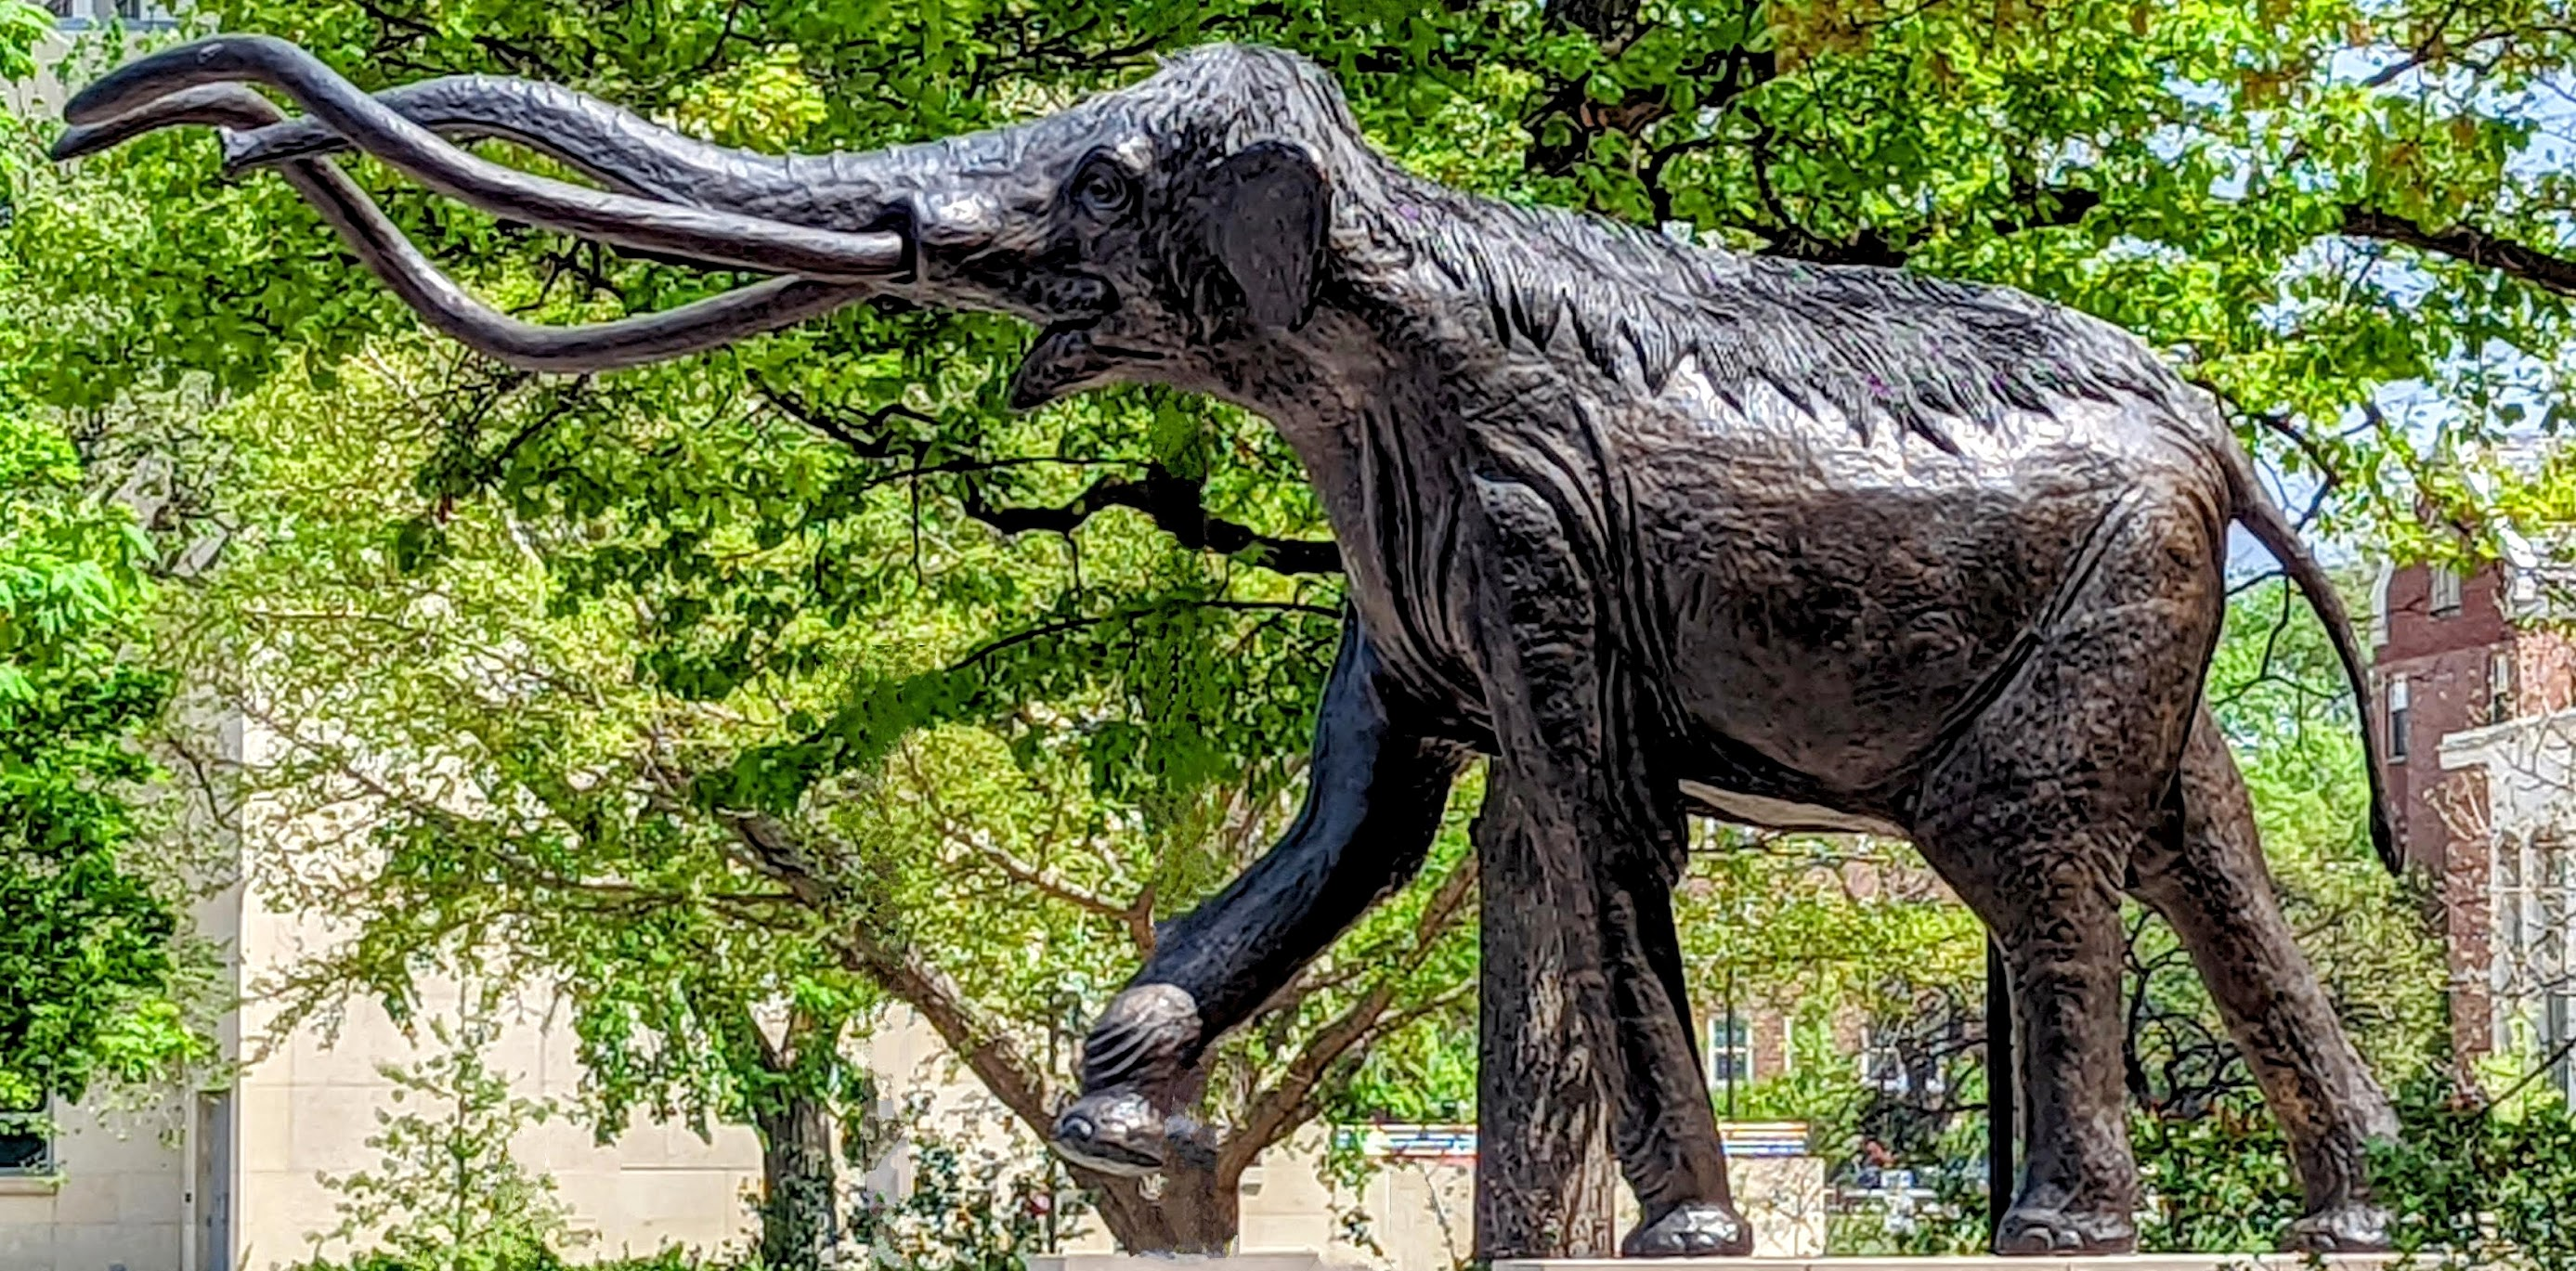
\includegraphics[width=.4\textwidth]{archie}
        \caption{Archie.\\ \footnotesize{Photograph by Bohn.}}
    \end{wrapfigure}

    You're relaxing at your favorite hangout when another customer catches your attention.
    He's rather large (dare I say, \textit{mammoth}), a bit hairy, and looking frustrated in front of his laptop.
    ``I'm Archie,'' he says, ``and I'm trying to teach myself this card game called \textit{Poker}.
    I found this source code that I thought I could use to understand Poker better, but the code is incomplete, and I don't entirely understand what's there.
    Could you explain the code to me, please?'
}

\newcommand{\GetHired}{
    Archie's face lights up in a very big smile.
    ``Thanks!''
    After pausing in thought for a moment, he says, ``Say, I've got a new startup company that could really use your help.
    Are you interested?
    It'll be exciting!''
}

\newcommand{\FirstDayOnTheJob}{
    \begin{wrapfigure}{r}{0.33\textwidth}
        \centering
        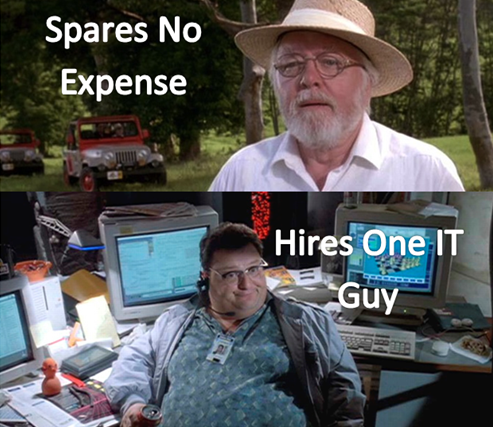
\includegraphics[width=.4\textwidth]{some-expenses-spared}
        \caption{Some expenses were spared.\\ \footnotesize{Original images \textcopyright\ Universal Studios and Amblin Entertainment, Inc. Meme creator unknown.}}
    \end{wrapfigure}

    You've recently been hired to help get the Pleistocene Petting Zoo get started.
    Your new employer, Archie, is surprisingly honest: he admits to you that some expenses were spared.
    Archie cheerfully points out that any challenge is also an opportunity to succeed.
    You suspect your job will offer plenty of ``opportunities to succeed.''
}

\newcommand{\HasKeyboard}{
    Great news!
    Archie brings you your new keyboard.
    He also brings you a problem of his own.
    Because you were held up with the broken keyboard, Archie decided to try some programming on his own, and his code is behaving strangely.
}

\newcommand{\ArchieWroteSmellyCode}{
    Working at the Pleistocene Petting Zoo certainly is proving to be interesting.
    You're glad that you don't have to worry about the problem of the giant sloths very slowly chasing their handlers, but now it seems that Archie has decided to try to write a program or two.
    At a glance, his code is smellier than the wooly rhinoceros' enclosure.
    But you take a closer look anyway to try to understand why his code acts strangely.
}

\newcommand{\InsurancePreview}{
    You hear somebody enter the room.
    ``\textit{Frankenstein}, `boat','' is the challenge, and she answers, ``borne.''
    Archie introduces you to the new arrival, ``Lil, this is our new developer, the one who wrote the app we just used.''
    He turns to you: ``This is Lilith Redd from business operations.''
    He turns back to her and continues, ``Lil, what's the good word?''

    ``The word isn't good, I'm afraid.
    I just heard back from the insurance company.''
}

\newcommand{\OnLoanToEclecticElectronics}{
    All work at the Pleistocene Petting Zoo has stopped while Archie tries to find a $\cancelto{\mathrm{reasonable}}{\mathrm{gullible}}$ insurance company.
    Rather than furloughing staff, he's asked everybody to help out with his other startup companies for a week or two.
    He specifically asked that you help out with Eclectic Electronics.

    Herb Bee, the chief engineer, explains that Eclectic Electronics is developing a patent-pending C-licon tool that will convert C code into an integrated circuit that has the same functionality as the original C code.
    To test it out, he tasked you with writing the code to implement an Arithmetic Logic Unit (ALU).
    Your task will be to implement integer addition, subtraction, multiplication, and division.
    Even though high-level languages' \textit{logical} boolean operations normally are not part of an ALU, Herb wants you to include these in the ALU to see if that can make some programs run faster.
    Because bitwise operations and bit shift operations have been implemented, you will be able to use C's bitwise and bit shift operators, but because arithmetic operations have not yet been implemented, you cannot use C's arithmetic operators.
    Because C library functions generally make use of arithmetic operations (which have not yet been implemented), you cannot use library functions.
}

\newcommand{\SuccessfulALU}{
    Herb smiles as he hands you the the test results from the latest integrated circuit fab batch.
    ``C-licon successfully turned your code into an ALU.
    Nicely done!''
    I think maybe it's time to use C-licon to see if we can improve the Floating Point Unit (FPU) on our experimental microprocessor.
}

\newcommand{\WriteAnFPU}{
    Herb tells you that, Eclectic Electronics tested the integrated circuit that the C-licon tool created from your ALU code, and they've concluded that C-licon is ready to use for their new experimental microprocessor.
    He tasks you with writing C code (that will be used by the C-licon tool) to implement a Floating Point Unit (FPU).
    Your task will be to implement floating point addition, subtraction, multiplication, and division.
    You can use any bit operations and, thanks to the ALU you wrote, you can use any integer arithmetic operations (use the conventional + - * / operators).
    Because the FPU has not yet been implemented, you cannot use C's floating point operations, you cannot use \lstinline{float}s nor \lstinline{double}s, and you cannot use library functions.
}

\newcommand{\GoingBackToTheZoo}{
    Lil enters the room.
    Herb challenges her: ``\textit{Gulliver's Travels}, `endian','' and Lil answers, ``ends.''

    Lil walks up to you and says, ``We have the insurance situation taken care of, and it's time to get the Zoo ready for guests.
    We're reassembling the tech team, and there's plenty of work to do.''

    You smile.
    ``That's good news!''

    Lil's face is hard to read.
    ``Well, yes and no.
    It's good that you'll be able to resume work on the Zoo's systems.
    But while Archie was waiting for us to fix the insurance situation, he got bored and -- cutting a long story short -- he ended up creating some new `opportunities' that we need you `to succeed' at.''
}

\newcommand{\SettledIntoRoutine}{
    You've settled into a comfortable routine at the Pleistocene Petting Zoo.
    While your job isn't quite as exciting as that of the saber-toothed tigers' dentist, it still has something new and interesting almost every day.

    Archie announces that he heard that hand-crafted assembly code can be faster than high-level language code.
    You try to explain that while this may have been true decades ago, modern optimizing compilers generate code faster than what a typical programmer can achieve with assembly code.
    Archie doesn't believe you and insists that you write the zoo's new cipher program in x86 assembly code.
}

\newcommand{\NewmanRanOffWithSamples}{
    Archie is hurriedly packing is trunk, like he's about to leave on a short-notice urgent trip.
    Before charging out the door, he pauses to tell you, ``Newman just stole some of our samples.
    I need to track him down before he sells them to the Supersized Safari Syndicate.
    I guess this means you're in charge of the Zoo's computer system now.
    Don't worry, you'll be fine. What could possibly go wrong?''
}

\newcommand{\BombLabIntroduction}{  % Ties Bryant & O'Halloran's Bomb Lab into the Pleistocene Petting Zoo story
    In a jarring collision of movie franchises, the CEO of Virtucon makes a Zoom call to the Pleistocene Petting Zoo.
    For some reason that nobody really explains, you're the only person available to handle the situation.
    The guy, who sounds kind of like an animated ogre, demands that the Pleistocene Petting Zoo deliver to him a megalodon shark with a head-mounted laser capable of emitting a beam of pure antimatter.

    You blurt out, ``Then it's not a laser,'' and then try to explain to him that megalodons are from the Miocene epoch, and expecting to find them at the Pleistocene Petting Zoo would be as ridiculous as a Cretaceous-period tyrannosaur at a Jurassic-themed park.

    ``Zip it!'' commands the guy who kind of looks like the host of a public-access show you used to watch.
    ``Since you won't meet my demand, my minions have placed a `binary bomb' under your zoo.
    Because I like really convoluted plans, we put software on your Linux server that controls the bomb.
    If you do nothing, the bomb will explode.
    If you turn off the Linux server, the bomb will explode.
    If you go slower than 50mph, the bomb will -- no, never mind that last part.

    ``The bomb software consists of a sequence of phases.
    Each phase expects you to type a particular string on \texttt{stdin}.
    If you type the correct string, then the phase is {\em defused} and the bomb proceeds to the next phase. Otherwise, the bomb {\em explodes}.
    The bomb is defused when every phase has been defused.

    ``Your mission, which you have no choice but to accept, is to defuse your bomb before the due date.
    Good luck, and welcome to the bomb squad!''
}

\newcommand{\FoodLockersAreStuck}{
    Having saved the Zoo from Dr. Evil's binary bomb, you relax back in your chair and think about taking a break.
%SPRINGBREAK
    Maybe an entire week in which you don't have solve any problems or meet any deadlines -- that'd be real nice.
%FALLBREAK
    % Maybe 4-day weekend in which you don't have solve any problems or meet any deadlines -- that'd be real nice.

    Another Zoom call comes in.
    \textit{What now!?} you wonder as you take your feet off of the desk to answer the call.
    An uncomfortable-looking animal handler says, ``We can't unlock the food lockers.
    It's the animals' feeding time, and we can't open the food lockers!
    It's feeding time, we can't get to the animals' food, and,'' his eyes dart nervously toward the animal enclosures, ``and many of them have sharp, pointy claws and others have big, stompy feet.''
}

\newcommand{\AttackLabIntroduction}{    % Ties Bryant & O'Halloran's Attack Lab into the Pleistocene Petting Zoo story
    You managed to keep the Pleistocene Petting Zoo from blowing to smithereens, but it turns out that Dr. Evil's minions weren't too careful when they put the bomb control software on the Zoo's Linux server.
    The software that controls the food locker has been heavily damaged!
    The functions that unlock the food locker doors are still present, but there's no way to activate those functions.

    You then recall what Archie told you when he hired you: some expenses were spared.
    You run the machine code through a disassembler and quickly see that it has a buffer overflow vulnerability.
    Before the situation in the dire wolf enclosure gets too dire, you sit down and get to work.

    The \function{ctarget} code runs on an older machine that allows executable code to be present on the stack, so it's vulnerable to a conventional code injection buffer overflow attack.
    \begin{itemize}
        \item Phase 1 (\function{touch1}) unlocks the food locker so the animal handlers can prepare the food.
        \item Phase 2 (\function{touch2}) opens the doors between the food locker and the carnivore enclosures;
        you will need to pass a cookie to the function to authenticate yourself.
        \item Phase 3 (\function{touch3}) closes the doors between the food locker and the carnivore enclosures.
    \end{itemize}
    The \function{rtarget} code runs on a newer machine that does not allow executable code to be present on the stack, so you'll have to conduct a return-oriented programming attack on it.
    \begin{itemize}
        \item Phase 4 (\function{touch2)} opens the doors between the food locker and the herbivore enclosures;
        you will need to pass a cookie to the function to authenticate yourself.
        \item Phase 5 (\function{touch3}) closes the doors between the food locker and the herbivore enclosures.
    \end{itemize}
}

\newcommand{\MostAnimalsAreFed}{
    Before you take on the Phase 5, pause to consider what you have accomplished so far.
    In Phases 2 and 3, you caused a program to execute machine code of your own design.
    If {\sc ctarget} had been a network server, you could have injected your own code into a distant machine.
    In Phase 4, you circumvented two of the main devices modern systems use to thwart buffer overflow attacks.
    Although you did not inject your own code, you were able inject a type of program that operates by stitching together sequences of existing code.
    Also, all animals have been fed, the carnivores are still in their enclosure, the mammoths can't fit through the herbivore door, and only the giant sloths seem interested in very slowly escaping.
}

\newcommand{\ArchieReturns}{
    Archie returns from tracking down Newman, who'd run off with some of the Pleistocene Petting Zoo's samples shortly before Dr.~Evil's Zoom call.
    ``It turns out he didn't get very far at all,'' Archie sighs.
    ``He ran into a flock of terror birds as he was leaving, and we found him in one of the emergency shelters.

    Archie smiles. ``I trust things were uneventful while I was away?''
}

\newcommand{\PickingUpNewmansProject}{
    Archie seems genuinely surprised that Newman is refusing to go back to work.
    ``You would think that he'd be grateful for being rescued from that flock of terror birds.''
    Before you can wonder out-loud whether it would be a good idea to trust someone who had just tried to sell trade secrets to a competitor, Archie gives you your new task.

    ``Because Newman isn't cooperating, I need you to finish the project he was working on.
    As you can imagine, duplicating the genetic information for our exhibits can take a long time, and Newman realized that we might be able to duplicate the data faster if we had a concurrent program which has one thread reading from the original data and another thread writing the copy.
    Unfortunately, he ran off to sell samples to the  Supersized Safari Syndicate before finishing the duplicator.
    Right now the duplicator seems to work, but it usually makes imperfect copies.
    Have you ever seen a paleolama with two noses, four eyes, and no ears!?''
}

\newcommand{\WeNeedBetterDetection}{
    Between Newman trying to sell samples to a competitor, that weird guy almost blowing up the zoo, and the animals almost escaping, Archie is getting worried.
    ``I think we need to introduce additional protective measures.
    As useful as your challenge-response app is in helping us detect intruders, I think it's now clear that we need something that will detect someone -- or some\textit{thing} -- when they're someplace they shouldn't be, even when no one else is around.
    I've asked the team at Eclectic Electronics to put something together.''
}

\newcommand{\WeNeedBetterLocks}{
    Between Newman trying to sell samples to a competitor, that weird guy almost blowing up the zoo, and the animals almost escaping, Archie is getting worried.
    ``I think we need to introduce additional protective measures.
    As useful as your challenge-response app is in helping us detect intruders, I think it's now clear that we need something that will keep someone -- or some\textit{thing} -- out of places they shouldn't be, even when no one else is around.
    I've asked the team at Eclectic Electronics to put something together.''
}

\newcommand{\IntroduceHardware}{
    Archie walks up to you, along with Herb Bee from Eclectic Electronics.
    Herb is holding a tangled mess of electronics.
    Archie explains, ``Herb here has developed a prototype of a device that he thinks will be useful for our physical security needs, as well as a few other applications around here. He calls it the \textit{Cow Pi}.''

% TODO: parameterize based on which microcontroller is actually being used
    You look at the device in Herb's hands and see the \nano\ central to the circuit.
    ``Isn't \textit{-Pi} typically used as a suffix for circuits that use a Raspberry Pi instead of an Arduino?''

    Herb replies, ``Typically, yes, but \textit{Cowduino} isn't very punny, is it?''

    Archie chimes in, ``Maybe with the right emphasis: \textit{Cow-DOO-ino}.''

    ``That's kind of subtle, don't you think? How will people know to put the emPHAsis on that sylLAble?''

    ``I think we're getting off topic here,'' you point out.
    ``How can I help?''

    ``Oh, right,'' Herb says, ``We'd like you to kick its proverbial tires.
    Let's start off with something simple, like a number builder tool.''
}

\newcommand{\JeffGoldblum}{
    Herb looks over your work.
    ``Hmm, yes. I think this is coming along nicely.
    Let's run a few more tests.''

    Archie storms into the room.
    ``We have \textit{got} to do something about security!
    How's that doodad coming along?
    Because there's now a half-man/half-fly in the labs going on-and-on about Chaos Theory and how if we just give him a MacBook and a spaceship then he'll be able to get the Lord of Thunder to travel across the 8th Dimension.
    Is that thing just about ready?''

    Herb shakes his head, ``No, not quite yet. It should be ready in about a week.''
}

\newcommand{\DisdainfulHerb}{
    Smoke wafts from Herb's soldering iron as he looks up when you approach.
    Cleaning the iron's tip, he quotes:
    ``Somebody once said, `The three most dangerous things in the world are a programmer with a soldering iron, a hardware engineer with a software patch, and'{}'' -- he glances nervously in Archie's direction -- ``{}`a user with an idea.'\footnote{
        Rick Cook, \textit{The Wizardry Consulted}, 1995.
    }$^{\mathrm{,}}$\footnote{
        The notion of being wary of programmers wielding screwdrivers or soldering irons long pre-dated this quote, as there are apocryphal tales of people who found it easier to modify the hardware to suit the software rather than the other way around.
    }''
}

\newcommand{\NumberConversionTool}{     % Since we're now allowing `sprintf()` with the LCD1602, converting between decimal and hexadecimal is trivial; it still might be okay for 7-segment displays
    Herb gets straight to the point.
    ``We promised Archie that we'd be able to start using the Cow Pi to build systems in a week.
    So far we've tested its input/output functionality, but we still need to test its timer and also whether we can take inputs without constantly polling the input devices.
    As before, we don't need to do anything too fancy;
    let's try a number base conversion tool.''
}

\newcommand{\LessDisdainfulHerb}{
    Smoke wafts from Herb's soldering iron as he looks up when you approach.
    Cleaning the iron's tip, he notes:
    ``Somebody once said that one of the most dangerous things in the world is a programmer with a soldering iron.''\footnote{
        ``The three most dangerous things in the world are a programmer with a soldering iron, a hardware engineer with a software patch, and a user with an idea.'' -- Rick Cook, \textit{The Wizardry Consulted}, 1995.
    }$^{\mathrm{,}}$\footnote{
        The notion of being wary of programmers wielding screwdrivers or soldering irons long pre-dated this quote, as there are apocryphal tales of people who found it easier to modify the hardware to suit the software rather than the other way around.
    }
}

\newcommand{\RemoteControlledCar}{

    About this time, Archie walks by, thinking about electric carts to transport visitors around the Pleistocene Petting Zoo.
    ``They probably should be remote-controlled.''
    He looks at you and Herb, and asks, ``Do you think you could make a cart a remote-controlled cart?''

    You ask the obvious question, ``Are there carts here already?''

    Archie waves his hand in the air, dismissing that detail, ``Not yet, but could you make the remote-control?''
    
    You hestatingly summarize: ``You want a cartless remote-controlled cart?''

    Archie beamingly smiles, ``Exactly!''

    Herb jumps in, ``Yes, we'll do it.''
    Herb looks at you and adds, ``It'll give us a chance to test the Cow Pi's timer and whether we can take inputs without constantly polling the input devices.''
}

\newcommand{\LauraDern}{
    You and Herb look for Archie in the Pleistocene Petting Zoo's labs to give him the good news, and you find a blond woman wearing cargo shorts, butchering a Gilbert and Sullivan song\dots \\ \\
    \textmusicalnote\ I am the very model of a modern vice admiral \textmusicalnote \\
    \textmusicalnote\ I've information about all things paleobotanical \textmusicalnote \\
    \textmusicalnote\ And I've been up to my armpits in problems scatological \textmusicalnote \\
    \textmusicalnote\ During the regency I had experience matriarchical \textmusicalnote \\
    \textmusicalnote\ I plot space travel, normal and superluminal \textmusicalnote \\
    \textmusicalnote\ (Even if I challenge the Pauli exclusion principle) \textmusicalnote \\

    ``I don't know how these people keep getting into our labs.
    \textit{Please} tell me that you have good news,'' pleads Archie.

    ``Yes, the Cow Pi is ready for whatever you need: calculators, security systems, parking meters -- you name it,'' Herb cheerfully responds.

    ``Excellent.''
    Archie turns to you.
    ``I'd like you and Newm... no, \textit{not} Newman.
    I'd like you and someone else on the staff to get started right away.
    Here's what I'd like to have built first.''
}

\newcommand{\CalculatorNeeded}{
    ``I have various teams working on different projects around here to improve security,'' Archie reminds you.
    He glances toward the Zoo's labs, where there's now a guy who looks like the actor who portrayed the fictional actor who portrayed the Norse god Odin, trying to avoid children while wistfully talking about raising rabbits in Montana.
    You briefly wonder why there are children someplace where there are also carnivorous megafauna, and then you remember that you work at a petting zoo.
    ``What I need your team to do,'' Archie continues, ``is make a four-function calculator so that we can quickly and easily determine whether we have the correct number of specimens, or if any are missing.''
}

\newcommand{\CalculatorCounting}{
    Technicians are using your calculator to compute how many specimens are still present in the lab, and establish that all specimens are accounted for after Newman's attempted theft.
    As reports come in of facilities getting secured with Cow Pi-based locks and passages being monitored with Cow Pi-based motion sensors, Archie smiles and tells you that this was a job well done.
    With all of the excitement neatly wrapped-up and arriving at a satisfactory conclusion, you look forward to a boring career in which there's absolutely no screaming and running for your life.
}

\newcommand{\CombinationLockNeeded}{
    ``I have various teams working on different projects around here to improve security,'' Archie reminds you.
    He glances toward the Zoo's labs, where there's now a guy who looks like the actor who portrayed the fictional actor who portrayed the Norse god Odin, trying to avoid children while wistfully talking about raising rabbits in Montana.
    You briefly wonder why there are children someplace where there are also carnivorous megafauna, and then you remember that you work at a petting zoo.
    ``What I need your team to do,'' Archie continues, ``is make a combination lock so that only authorized people can get into our lab facilities.''
}

\newcommand{\CombinationLockInstalled}{
    After fastening the new electronic combination lock to the lab door, Archie smiles and tells you that this was a job well done.
    With all of the excitement neatly wrapped-up and arriving at a satisfactory conclusion, you look forward to a boring career in which there's absolutely no screaming and running for your life.
}

\newcommand{\RangeFinderNeeded}{
    ``I have various teams working on different projects around here to improve security,'' Archie reminds you.
    He glances toward the Zoo's labs, where there's now a guy who looks like the actor who portrayed the fictional actor who portrayed the Norse god Odin, trying to avoid children while wistfully talking about raising rabbits in Montana.
    You briefly wonder why there are children someplace where there are also carnivorous megafauna, and then you remember that you work at a petting zoo.
    ``What I need your team to do,'' Archie continues, ``is make a range finder that will alert us when someone -- or some\textit{thing} -- gets too close to someplace they shouldn't be.''
}

\newcommand{\RangeFinderDetecting} {
    A technician installing a new range finder outside the lab door briefly sets off the alarm, but then the range finder falls quiet and faithfully reports that nothing is approaching.
    As reports come in of facilities getting secured with Cow Pi-based locks, and of accurate speciment counts accomplished with Cow Pi-based calculators, Archie smiles and tells you that this was a job well done.
    With all of the excitement neatly wrapped-up and arriving at a satisfactory conclusion, you look forward to a boring career in which there's absolutely no screaming and running for your life.
}

\usepackage{amsmath}
%\usepackage{array,color,colortbl}
\definecolor{LightGreen}{rgb}{0.88,1,0.88}
\usepackage{multicol}
\usepackage{CJKutf8}
\usepackage{gensymb}
\usepackage{graphicx}
\usepackage{multirow}
\usepackage{listings}
\usepackage{tikz}
\setlength{\columnsep}{2cm}
\newcommand{\power}{power~({\color{red}\textbf{+}}) rail}
\newcommand{\ground}{ground~({\color{blue}\textbf{--}}) rail}



\captionsetup{width=.8\linewidth}

\lstset{language=c, numbers=left, showstringspaces=false,
    moredelim = [s][\ttfamily]{/*}{*/} % I shouldn't need this parameter!
}

\renewcommand{\labnumber}{\capstonelabnumber}
\renewcommand{\labname}{Implementing a Combination Lock}
\renewcommand{\shortlabname}{combolock -- grouplab}
\renewcommand{\collaborationrules}{\capstonelabcollaboration}
\renewcommand{\duedate}{\capstonelabdue}
\renewcommand{\runtimeenvironment}{\capstonelabenvironment}
\pagelayout
\begin{document}
    \labidentifier

    \pdfbookmark[1]{Frontmatter}{frontmatter}                           In this assignment, you will write code for \runtimeenvironment\ that will use new electronic devices to interact with the physical world.

The instructions are written assuming you will edit the code in the Arduino IDE and run it on \runtimeenvironment, constructed according to the pre-lab instructions.
If you wish, you may edit the code in a different environment; however, our ability to provide support for problems with other IDEs is limited.

\section*{Learning Objectives}

After successful completion of this assignment, students will be able to:
\begin{itemize}
    \item Work collaboratively on a hardware/software project
    \item Design and implement a simple embedded system
    \item Expand their programming knowledge by consulting documentation
\end{itemize}

\subsection*{Continuing Forward}

This penultimate lab assignment does not contribute to the final lab assignment.
By integrating elements of what you learned in this course, and by demonstrating that you can review documentation to learn on your own, to design a small embedded system, you will show how much progress you have made this semester.

\section*{During Lab Time}

During your lab period, coordinate with your group partner(s) to decide on your working arrangements.
Unless you're only going to work on the assignment when you're together, you may want to set up a private Git repository that is shared with your partner(s).
With your partner(s), modify your hardware kit as described in Section~\ref{sec:hardwareMods}.
Then, think through your system's design and begin implementing it.
The TAs will be available for questions.


    \softwareengineeringfrontmatter

    \section*{Scenario}                                                 \CombinationLockNeeded

    \section{Assignment Summary}                                        This assignment is principally about getting comfortable when explicitly working with memory.
Being able to think about a value and a reference to that value distinctly will improve your programming skills in any language.

Before you do so, in Section~\ref{sec:archiesCode} you will examine Archie's code.
Parts of Archie's programs use code that the C standard explicitly states will result in undefined behavior.
By understanding the mistakes that Archie made, we hope that you can avoid them in your own code.

In Section~\ref{sec:challengeResponse}, you will build and use a linked list.
This will require you to allocate space for the list's nodes and manipulate pointers that connect the nodes to each other.

\ifboolexpe{not bool{allowspaghetticode}}{
    There are no particular restrictions in this assignment other than those common to most lab assignments in this course.
    You can check whether you're using a \lstinline{goto} or \lstinline{continue} statement, or whether you're using \lstinline{break} or \lstinline{return} to exit a loop, by running the constraint-checking Python script:
    \texttt{python constraint-check.py linkedlistlab.json}
}{}


    \section{Getting Started} \label{sec:GettingStarted}                Download \textit{\shortlabname.zip} or \textit{\shortlabname.tar} from \filesource\ and copy it to \runtimeenvironment.
Once copied, unpackage the file.
Four of the five files (\textit{alu.h}, \textit{basetwo.c}, \textit{alu.c}, and \textit{integerlab.c}) contain the starter code for this assignment.
The last file (\textit{Makefile}) tells the \texttt{make} utility how to compile the code.
To compile the program, type:

\texttt{make}

This will produce an executable file called \textit{integerlab}.

When you run the program with the command \texttt{\textbf{\textit{./integerlab}}}, you will be prompted:

\begin{verbatim}
    Enter a one- or two-operand logical expression,
        a two-operand comparison expression, a two-operand arithmetic expression,
        "lg <value>" or "exponentiate <value>" to test your powers-of-two code,
        "is_negative <value>" to determine if 2's complement value is negative,
        "add1 <binary_value1> <binary_value2> <carry_in>" for 1-bit full adder,
        "add32 <hex_value1> <hex_value2> <carry_in>" for 32-bit ripple-carry adder,
        or "quit":
\end{verbatim}

When you enter a value, if it is prepended with \texttt{\textbf{\textit{0x}}} then the parser will parse it as a hexadecimal value;
otherwise, except as noted in Sections~\ref{subsec:one-bit-full-adder} and \ref{subsec:ripple-carry-adder}, the parser will treat it as a decimal value.

For now, type \texttt{\textbf{\textit{quit}}} to exit the program.

\subsection{Description of IntegerLab Files}

\subsubsection{integerlab.c}

Do not edit \textit{integerlab.c}.

This file contains the driver code for the lab.
It parses your input, calls the appropriate arithmetic function, and displays the output.

\subsubsection{alu.h} \label{subsubsec:alu.h}

Do not edit \textit{alu.h}.

This header file contains two type definitions:
\begin{description}
    \item[one\_bit\_adder\_t] is a structure to hold the 1-bin inputs (\lstinline{a}, \lstinline{b}, \lstinline{c_in}) and 1-bit outputs (\lstinline{sum}, \lstinline{c_out}) of a one-bit full adder.
    \item[alu\_result\_t] is a structure to hold the outputs from an arithmetic logic unit.
        Its fields are:
        \begin{itemize}
            \item \lstinline{result}, a 16-bit bit vector that is considered ``the'' result of the computation
            \item \lstinline{supplemental_result}, a 16-bit bit vector that stores additional result data from instructions that place their results in two registers
            \item \lstinline{unsigned_overflow}, a 1-bit flag to indicate whether overflow occurred when interpreting the source operands as unsigned values
            \item \lstinline{signed_overflow}, a 1-bit flag to indicate whether overflow occurred when interpreting the source operands as signed values
            \item \lstinline{divide_by_zero}, a 1-bit flag to indicate whether there was an attempt to divide by zero.
        \end{itemize}
\end{description}

The header file also contains two macros, \function{is_zero()} and \function{is_not_zero()} to bootstrap your ALU code.
These macros act like functions and return a boolean value to indicate whether an integer is 0 or not.\footnote{
    The astute student will quickly realize that \function{is_not_zero()} is not necessary and, with a little thought, will realize that they can \function{is_zero()} as a function within the constraints of this assignment.}

The header file also contains several function declarations.
The requirements for these functions will be discussed later in this assignment.

\subsubsection{basetwo.c}

This is the first of two files that you will edit.

There are two functions in \textit{basetwo.c} that will allow you to demonstrate an understanding of powers-of-two and/or an understanding of some uses of bit shifts.
\begin{description}
    \item[lg()] returns the base-2 logarithm of its argument, assuming its argument is a positive power-of-two;
        if the argument is 0 or is not a power-of-two, then there are no guarantees about the function's return value
    \item[exponentiate()] creates a power-of-two by raising 2 to the provided exponent, assuming the exponent is a non-negative value strictly less than 32;
        if the argument is negative or is greater than 31, then there are no guarantees about the function's return value
\end{description}
These functions are inverses of each other: $x = \log_2 2^x$, and $y = 2^{\log_2 y}$.

Strictly speaking, you can write your ALU code without these functions;
however, some students in the past had difficulty finding solutions for their ALU code without obtaining a base-2 logarithm and/or calling a function to create a power-of-two.
Rather than tempt you to violate one of the assignment's constraints by calling the \textit{math} library's \function{log2()}, \function{exp2()}, and/or \function{pow()} functions, we now have you write your own code for these functions.

\subsubsection{alu.c}

This file will contain most of the code that you write, and the functions in \textit{alu.c} are in the order in which you will likely write them.
\begin{itemize}
    \item A simple check
        \begin{description}
            \item[is\_negative()] returns a boolean value to indicate whether the argument, when interpreted as a signed integer, is negative
        \end{description}
    \item Equality comparisons
        \begin{description}
            \item[equal()] returns \lstinline{true} if and only if $value1 = value2$
            \item[not\_equal()] returns \lstinline{true} if and only if $value1 \not = value2$
        \end{description}
    \item Logical operations
        \begin{description}
            \item[logical\_not()] returns the logical inverse of the argument
            \item[logical\_and()] returns the logical conjunction of the two arguments
            \item[logical\_or()] returns the logical disjunction of the two arguments
        \end{description}
    \item Addition and subtraction
        \begin{description}
            \item[one\_bit\_full\_addition()] performs addition for one bit position, determining both the sum bit and the carry-out bit
            \item[ripple\_carry\_addition()] adds two 32-bit values to each other and to a carry-in bit
            \item[add()] adds two 16-bit values to each other
            \item[subtract()] subtracts a 16-bit value from another
        \end{description}
    \item Inequality comparisons
        \begin{description}
            \item[less\_than()] returns \lstinline{true} if and only if $value1 < value2$
            \item[at\_most()] returns \lstinline{true} if and only if $value1 \leq value2$
            \item[at\_least()] returns \lstinline{true} if and only if $value1 \geq value2$
            \item[greater\_than()] returns \lstinline{true} if and only if $value1 > value2$
        \end{description}
    \item Unsigned multiplication and division
        \begin{description}
            \item[multiply\_by\_power\_of\_two()] multiplies the first argument by the second, assuming that the second argument is zero or a power of two;
                there are no guarantees if this assumption is not satisfied
            \item[unsigned\_multiply()] multiplies two 16-bit values to each other, if the arguments are interpreted as unsigned integers
            \item[unsigned\_divide()] divides a 16-bit value by another, if the arguments are interpreted as unsigned integers
        \end{description}
    \item Signed multiplication and division (bonus credit)
    \begin{description}
        \item[signed\_multiply()] multiplies two 16-bit values to each other, if the arguments are interpreted as signed integers
        \item[signed\_divide()] divides a 16-bit value by another, if the arguments are interpreted as signed integers
    \end{description}
\end{itemize}


    \vspace{1cm}

    After you have assembled the hardware, you can work on the lab entirely with your partner, perhaps pair programming,
    or you can decide to have one partner work on Section~\ref{sec:rotaryEncoder} and the other work on Section~\ref{sec:servo}.
    Regardless, you will need to work together on Section~\ref{sec:integration}, as this is when you will integrate the work from Sections~\ref{sec:rotaryEncoder}--\ref{sec:servo}.

    \section{Test Mode Specification} \label{sec:testMode}              If the \textbf{right switch} is in the \textit{left position} when the system boots, then the system shall enter its test mode.
The test mode is used to demonstrate the correct handling of the \textbf{rotary encoder} and of the \textbf{servomotor}.

\subsection*{When the system is in its test mode:}
%! suppress = LabelConvention
\begin{enumerate}
    \item \label{spec:encoderCounts} The system shall display the number of times that the \textbf{rotary encoder} is turned clockwise and the number of times that the \textbf{rotary encoder} is turned counterclockwise.
%        \begin{itemize}
%            \item Optionally, the system may also display the quadrature values as the \textbf{rotary encoder is turned}.
%        \end{itemize}
    \item \label{spec:servoCenter} If the \textbf{right pushbutton} is \textit{pressed}, the servomotor shall take its \textit{center position}.
    \item \label{spec:servoFollow} If the \textbf{right pushbutton} is \textit{not pressed}, the servomotor shall follow the \textbf{left switch}:
        \begin{itemize}
            \item If the \textbf{left switch} is in the \textit{left position}, the servomotor shall rotate \textit{fully clockwise}.
            \item If the \textbf{left switch} is in the \textit{right position}, the servomotor shall rotate \textit{fully counterclockwise}.
        \end{itemize}
    \item \label{spec:servoString} The system shall display ``SERVO: center'', ``SERVO: left'', or ``SERVO: right'' according to the command given to the servo per Requirements~\ref{spec:servoCenter}--\ref{spec:servoFollow}.
\end{enumerate}


    \section{Rotary Encoder Test Mode} \label{sec:rotaryEncoder}        \subsection{Theory of Operation}

The rotary encoder consists of a shaft that can rotate without stop in either direction,
and detents that hold the shaft in position when you are not rotating it.
Electrically, it has a pair of wipers, each of which is connected to a pin at one end, and which share a common pin at the other end.
By connecting the common pin to ground (as we have) and connecting the wipers' pins to pulled-up input pins on the microcontroller (as we have), then we can read the logic values of the wipers.

As the shaft rotates, the pair of wipers each cycle through a square wave.
The two wipers' square waves form a \textit{quadrature};
that is, they are 90\textdegree out of phase with each other, as shown in Figure~{fig:quadrature}.
By tracking which pin changes value first or second, we can determine which direction the shaft is rotating.

\begin{figure}
    \begin{center}
        \begin{tikzpicture}[x=2mm, y=2mm]
            \draw (0,0) -- ++(2.5,0) -- ++(0,5) -- ++(5,0) -- ++(0,-5) -- ++(5,0) -- ++(0,5) -- ++(5,0) -- ++(0,-5) -- ++(5,0) -- ++(0,5) -- ++(5,0) -- ++(0,-5) -- ++(2.5,0);
            \draw (-5, 2.5) node[left]{B};
            \draw (-1, 0) node[left]{\small 0};
            \draw (-1, 5) node[left]{\small 1};
            \draw (0,0) ++(0,-10) -- ++(0,5) -- ++(5,0) -- ++(0,-5) -- ++(5,0) -- ++(0,5) -- ++(5,0) -- ++(0,-5) -- ++(5,0) -- ++(0,5) -- ++(5,0) -- ++(0,-5) -- ++(5,0);
            \draw (-5, -7.5) node[left]{A};
            \draw (-1, -10) node[left]{\small 0};
            \draw (-1, -5) node[left]{\small 1};
            \draw[-Latex] (10, 10) -- ++(5,0) node[right]{\footnotesize clockwise};
            \draw[Latex-] (10, 8) -- ++(5,0) node[right]{\footnotesize counterclockwise};
            \draw[dashed] (3.75, -11) -- ++(0, 21) node[above] {detent};
            \draw[dashed] (3.75, -11) ++(10, 0) -- ++(0, 17);
            \draw[dashed] (3.75, -11) ++(20, 0) -- ++(0, 17);
        \end{tikzpicture}
        \caption{Quadrature encoding of the rotational position in a rotary encoder.} \label{fig:quadrature}
    \end{center}
\end{figure}

\subsection{Changes to \textit{rotary-encoder.c}}

Open \textit{rotary-encoder.c}.
Locate the \function{get_quadrature()} function.
The \texttt{A} component of the signal from Figure~{fig:quadrature} is on input pin~16, and the \texttt{B} component is on input pin~17.
\begin{description}
    \checkoffitem{Read the quadrature from the input pins into a variable.}
    \checkoffitem{Shift the bits in that variable so that the \texttt{A} component is in bit~0 and the \texttt{B} component is bit 1, and return the shifted variable.}
\end{description}

We will track the movement of the rotary encoder's shaft using the state machine depicted in Figure~\ref{fig:rotaryEncoderStateMachine}.
The convention we will use is that the states are named after the logic values of the quadrature's two components: \texttt{\textit{B\_A}}.
For example, if the bits returned by \function{get_quadrature()} are 0b0000'0010 then the state machine should be in state \texttt{HIGH\_LOW}.

\begin{figure}
    \begin{center}
        \begin{tikzpicture}
            \node[state, initial]   at (0, 10)  (highHigh){HIGH\_HIGH};
            \node[state]            at (5, 5)   (highLow){HIGH\_LOW};
            \node[state]            at (-5, 5)  (lowHigh){LOW\_HIGH};
            \node[state]            at (0, 0)   (lowLow){LOW\_LOW};
            \draw   (highHigh)  edge[-Latex, bend left]     node{\rotatebox{-45}{\textcolor{blue}{quadrature==0b10}}}   (highLow)
                    (highHigh)  edge[-Latex, bend right]    node{\rotatebox{45}{\textcolor{blue}{quadrature==0b01}}}    (lowHigh)
                    (highLow)   edge[-Latex, bend left]     node{\rotatebox{-45}{\textcolor{blue}{quadrature==0b11}}}   (highHigh)
                    (highLow)   edge[-Latex, bend left]     node{\rotatebox{45}{\parbox{5cm}{\centering\textcolor{blue}{quadrature==0b00 \&\& last\_state==HIGH\_HIGH}\\\textcolor{red}{rotating clockwise} } } }           (lowLow)
                    (lowHigh)   edge[-Latex, bend right]    node{\rotatebox{45}{\textcolor{blue}{quadrature==0b11}}}    (highHigh)
                    (lowHigh)   edge[-Latex, bend right]    node{\rotatebox{-45}{\parbox{5cm}{\centering\textcolor{blue}{quadrature==0b00 \&\& last\_state==HIGH\_HIGH}\\\textcolor{red}{rotating counterclockwise} } } }   (lowLow)
                    (lowLow)    edge[-Latex, bend right]    node{\rotatebox{-45}{\parbox{5cm}{\centering\textcolor{blue}{\phantom{x} \\ quadrature==0b01 \&\& last\_state==HIGH\_LOW}}}}   (lowHigh)
                    (lowLow)    edge[-Latex, bend left]     node{\rotatebox{45}{\parbox{5cm}{\centering\textcolor{blue}{\phantom{x} \\ quadrature==0b10 \&\& last\_state==LOW\_HIGH}}}}    (highLow)
                    ;
        \end{tikzpicture}
        \caption{State machine to determine a rotary encoder's direction of rotation.}\label{fig:rotaryEncoderStateMachine}
    \end{center}
\end{figure}

Locate the \function{initialize_rotary_encoder()}
\begin{description}
    \checkoffitem{Initialize the \lstinline{state} variable.}
\end{description}

For test mode, we'll use \lstinline{clockwise_count} and \lstinline{counterclockwise_count} to count the number of times that the shaft is turned in each direction for Requirement~\ref{spec:encoderCounts}.
For the combination lock, we'll use \lstinline{direction} to track which direction the shaft was turned.
Once the direction has been provided to the lock controller, we want to set \lstinline{direction} back to \lstinline{STATIONARY} so that a single turn isn't interpreted as many turns.

Location \function{count_rotations()}.
\begin{description}
    \checkoffitem{Add code to populate the buffer with the counts as required by Requirement~\ref{spec:encoderCounts}.
        Clearly label which count is which.
        \begin{itemize}
            \item Due to the limited amount of space on the display, you'll probably want to abbreviate, such as ``CW'' for clockwise and ``CCW'' for counterclockwise.
        \end{itemize}
    }
    \checkoffitem{Compile and upload your code, and confirm that a descriptive string is displayed with the counts (both of which should be 0 for now).}
\end{description}

Locate \function{get_direction()}.
\begin{description}
    \checkoffitem{Add code to save a copy of \lstinline{direction}.}
    \checkoffitem{Add code to set \lstinline{direction} to \lstinline{STATIONARY}.}
    \checkoffitem{Return the copy of \lstinline{direction}.}
\end{description}

Locate \function{handle_quadrature_interrupt()} and examine the state machine depicted in Figure~\ref{fig:rotaryEncoderStateMachine}.
You will implement the state machine in \function{handle_quadrature_interrupt()},
but first make sure that you understand how the state transitions driven by the quadrature signal in Figure~\ref{fig:quadrature} allow us to determine the direction of rotation.

\subsubsection*{But what about debouncing?}

You \textit{should} be wondering about debouncing.
After all, the rotary encoder relies on mechanical contacts.
In fact the \texttt{A} and \texttt{B} wipers \textit{do} experience switch bounce.
Fortunately, the state machine provides us a way to implement debouncing without using \function{cowpi_debounce_byte()} or \function{debounce_interrupt()}.

Consider the transition from \texttt{HIGH\_HIGH} to \texttt{HIGH\_LOW}:
\begin{itemize}
    \item This could be due to the user turning the shaft clockwise, causing the \texttt{A} component to drop from 1 to 0, or
    \item This could be due to switch bounce
        \begin{itemize}
            \item The user has turned the shaft counterclockwise
            \item The last quadrature change from that action is the \texttt{A} component rising from 0 to 1
            \item Switch bounce has caused the \texttt{A} component to drop from 1 to 0
        \end{itemize}
\end{itemize}
Now consider the transition from \texttt{HIGH\_LOW} to \texttt{HIGH\_HIGH}:
\begin{itemize}
    \item This could be due to the user rotating the shaft counterclockwise, causing the \texttt{A} component to rise from 0 to 1, or
    \item This could be due to the \texttt{A} wiper bouncing back as part of the aforementioned switch bounce
\end{itemize}
The reasoning is similar for transitions between \texttt{HIGH\_HIGH} and \texttt{LOW\_HIGH}.

Now consider the transition from \texttt{HIGH\_LOW} to \texttt{LOW\_LOW}.
Continuing the clockwise turn, the \texttt{B} component drops from 1 to 0.
If the change in \texttt{B}'s value were due to switch bounce, then we shall deny the state transition.
How?
By remembering which state the state machine was in before it was in \texttt{HIGH\_LOW}.

If the previous state was \texttt{HIGH\_HIGH} then \texttt{we know that the shaft is turning clockwise}.
On the other hand, if the previous state was \texttt{LOW\_LOW} then we know that the \texttt{B} wiper is bouncing.
Thus, we will only allow a transition from \texttt{HIGH\_LOW} to \texttt{LOW\_LOW} if the previous state was \texttt{HIGH\_HIGH}.
We will similarly limit all transitions into and out of \texttt{LOW\_LOW}.

(We cannot similarly limit the transitions into and out of \texttt{HIGH\_HIGH} because after the shaft stops at the detent, the user can continue to turn the shaft in the same direction, or they could turn the shaft in the opposite direction.)

\begin{description}
    \checkoffitem{Implement the state machine from Figure~\ref{fig:rotaryEncoderStateMachine} in \function{handle_quadrature_interrupt()}.}
    \checkoffitem{Add code to the transitions into \texttt{LOW\_LOW} to update \lstinline{clockwise_count}, \lstinline{counterclockwise_count}, and \lstinline{direction} as appropriate.}
\end{description}

Locate the \function{initialize_rotary_encoder()} function:
\begin{description}
    \checkoffitem{Uncomment this line: \\
    \lstinline{//    register_pin_ISR((1 << A_WIPER_PIN) | (1 << B_WIPER_PIN), handle_quadrature_interrupt);}
    }
    \checkoffitem{Compile and upload your code, and confirm that the clockwise count and counterclockwise count update on the display as specified by Requirement~\ref{spec:encoderCounts}.}
        \begin{itemize}
            \item It is acceptable for the counter to fail to update for the occasional turn if you turn the shaft quickly, but slow turns should always register, and most fast turns should register.
        \end{itemize}
\end{description}


    \section{Servomotor Test Mode} \label{sec:servo}                    \subsection{Theory of Operation}

The servomotor is controlled with a signal that consists of periodic pulses.
The desired position of the servomotor is encoded as with width of each pulse.
This encoding, \textit{pulse width modulation} (PWM) is sufficiently useful that most microcontrollers can be configured to generate such a signal by setting a few of their memory-mapped I/O registers.
We will not do that.
Instead, we will directly form the signal by setting an output pin to 1 or 0 as needed.
Figure~\ref{fig:pwm} shows the relevant parameters of a PWM signal.

\begin{figure}
    \begin{center}
        \begin{tikzpicture}[x=2mm, y=2mm]
            \draw (0,0) -- (5,0) -- ++(0,5) -- ++(5,0) -- ++(0,-5) -- (25,0) -- ++(0,5) -- ++(5,0) -- ++(0,-5) -- (45,0)-- ++(0,5) -- ++(5,0) -- ++(0,-5) -- (65,0)-- ++(0,5) -- ++(5,0) -- ++(0,-5) -- (75,0);
            \draw (-1, 0) node[left]{\small 0};
            \draw (-1, 5) node[left]{\small 1};
            \draw (25, -3) -- ++(0,-6);
            \draw (45, -3) -- ++(0,-6);
            \draw[Latex-Latex] (26, -6) -- (44,-6) node[pos=.5]{\footnotesize \parbox{1.8cm}{\centering signal\\period}};
            \draw (45, 8) -- ++(0, 6);
            \draw (50, 8) -- ++(0, 6);
            \draw[Latex-] (44, 11) -- ++(-3, 0);
            \draw[Latex-] (51, 11) -- ++(3, 0);
            \draw (47.5, 11) node{\footnotesize \parbox{1.8cm}{\centering pulse\\width}};
        \end{tikzpicture}
        \caption{A PWM signal periodically sends a pulse. The $pulse\ width$ encodes the information being transmitted; the $signal\ period$ is how often the pulse is sent.}\label{fig:pwm}
    \end{center}
\end{figure}

A servomotor expects a pulse to be sent every 20ms (20,000\textmu s); this is the \textit{signal period}.
The \textit{pulse width} can vary between 500\textmu s and 2500\textmu s.
A 500\textmu s pulse directs the servomotor to rotate fully clockwise,
and a 2500\textmu s pulse directs the servomotor to rotate fully counterclockwise.
The angle varies linearly with the pulse width (for example, 1500\textmu is the central position).

\subsection{Changes to \textit{servomotor.c}}

Open \textit{servomotor.c}.

Locate these lines of code:
\begin{lstlisting}
#define PULSE_INCREMENT_uS  (INT32_MAX)
#define SIGNAL_PERIOD_uS    (INT32_MAX)
\end{lstlisting}
\begin{description}
    \checkoffitem{For \lstinline{SIGNAL_PERIOD_uS}, replace \lstinline{INT32_MAX} with the period (measured in microseconds) that the servomotor requires of its signal.}
    \checkoffitem{Select a factor common to the signal period and to each of the pulse widths necessary to realize Requirements~\ref{spec:servoCenter}--\ref{spec:servoFollow}.}
    \checkoffitem{For \lstinline{PULSE_INCREMENT_uS}, replace \lstinline{INT32_MAX} with that factor (measured in microseconds).
        This will be your timer interrupt period.}
\end{description}

Locate the \function{test_servo()} function.
\begin{description}
    \checkoffitem{Add code to call the \function{center_servo()}, \function{rotate_full_clockwise()}, and \\ \function{rotate_full_counterclockwise()} functions as necessary for Requirements~\ref{spec:servoCenter}--\ref{spec:servoFollow}.}
    \checkoffitem{Add code to populate \lstinline{buffer} with the strings required by Requirement~\ref{spec:servoString}.}
    \checkoffitem{Compile and upload your code, and confirm that the correct strings are displayed.}
\end{description}

Locate the \function{center_servo()}, \function{rotate_full_clockwise()}, and \function{rotate_full_counterclockwise()} functions.
\begin{description}
    \checkoffitem{Populate these functions with code to set the value of \lstinline{pulse_width_us} to the necessary pulse width as necessary to encode the servo's desired rotational position into the pulse width.}
\end{description}

Locate the \function{handle_timer_interrupt()} function.
\begin{description}
    \checkoffitem{Add variables to track the time until the next rising edge of the pulse and the next falling edge of the pulse.}
    \checkoffitem{Add code so that when the time until the next rising edge is 0\textmu s:
        \begin{itemize}
            \item Start the pulse by setting output pin~22 to 1.
            \item Update your variable that tracks the time until the next rising edge, to the time until the \textit{next} pulse should start.
            \item Update your variable that tracks the time until the next falling edge, to the time until \textit{this} pulse should finish.
        \end{itemize}
    }
    \checkoffitem{Add code so that when the time until the next falling edge is 0\textmu s:
        \begin{itemize}
            \item Finish the pulse by setting output pin~22 to 0.
        \end{itemize}
    }
    \checkoffitem{Add code to update the time remaining until the next rising edge and the time until the next falling edge, to reflect the time that has elapsed between timer interrupts.}
\end{description}

Locate the \function{initialize_servo()} function:
\begin{description}
    \checkoffitem{Uncomment this line: \\
        \lstinline{//    register_periodic_timer_ISR(0, PULSE_INCREMENT_uS, handle_timer_interrupt);}
    }
\end{description}

\vspace{1cm}

\textcolor{red}{Pre-emptive debugging.} Consider:
\begin{description}
    \checkoffitem{Multiply the definitions of \lstinline{SIGNAL_PERIOD_uS} and \lstinline{PULSE_INCREMENT_uS} by 1000.}
    \checkoffitem{Multiply the assignments to \lstinline{pulse_width_us} by 1000.}
    \checkoffitem{In \function{handle_timer_interrupts()}, replace the updates to pin~22 with updates to pin~20.}
\end{description}
This will have the effect of replacing ``microseconds'' with ``milliseconds'' and of replacing the servomotor with the right LED\@.
\begin{description}
    \checkoffitem{Compile and upload your code, and confirm that the correct right LED lights up and dims in the correct pattern, considering that you have replaced ``microseconds'' with ``milliseconds''.}
    \checkoffitem{Restore the original definitions, assignments, and pin number.}
\end{description}

\vspace{1cm}

\begin{description}
    \checkoffitem{Compile and upload your code, and confirm that the servomotor rotates to the correct positions as specified by Requirements~\ref{spec:servoCenter}--\ref{spec:servoFollow}.}
\end{description}


    \section{Combination Lock Specification} \label{sec:spec}           %! suppress = LabelConvention
\begin{enumerate}
    \item Definitions
        \begin{description}
            \item[Threshold Range] The distance at which a detected object will cause the system to produce an audible alarm
            \item[Strobe] An illumination of an LED for 50ms
            \item[Chirp] A 5kHz tone lasting 50ms
        \end{description}
    \item \label{spec:modes} The slide-switches shall control the mode of operation.
        \begin{enumerate}
            \item Both switches in the \textit{left position}: Normal Operation
            \item The \textbf{left switch} in the \textit{right position} and the \textbf{right switch} in the \textit{left position}: Single-Pulse Operation
            \item Both switches in the \textit{right position}: Threshold Adjustment
            \item The \textbf{left switch} in the \textit{left position} and the \textbf{right switch} in the \textit{right position}: Continuous Tone
        \end{enumerate}
    \item \label{spec:continuousTone} When the range finder and alarm system is in \textbf{Continuous Tone} mode:
        \begin{enumerate}
            \item The system shall not detect the range of nearby objects: it shall neither emit nor detect ultrasound
            \item The system shall not illuminate an LED
            \item The system shall produce a continuous 5kHz audible tone
        \end{enumerate}
    \item \label{spec:thresholdAdjustment} When the range finder and alarm system is in \textbf{Threshold Adjustment} mode:
        \begin{enumerate}
            \item The system shall not detect the range of nearby objects: it shall neither emit nor detect ultrasound
            \item The system shall not produce an audible tone
            \item The system shall not illuminate an LED
            \item The system shall prompt the user on the \textbf{display module} to enter the threshold range, in centimeters
                \begin{itemize}
                    \item You may assume that the user understands what the system does: the prompt must be \textit{meaningful}, but it may be \textit{succinct}
                \end{itemize}
            \item The user shall be able to enter the threshold range, in centimeters, using the numeric keypad
                \begin{enumerate}
                    \item The user will enter the range in decimal
                    \item The system shall echo the user's input, digit-by-digit, on the \textbf{display module} as they type their input
                    \item The user will indicate that they have finished entering their input by pressing the `\#' key
                \end{enumerate}
            \item After the user has completed their input, then any value less than 50cm or greater than 400cm shall be rejected as an invalid threshold;
                the system shall display a helpful error message on the \textbf{display module} and re-prompt the user to enter the threshold range
            \item After the user has completed their input, and if the input is valid, then the system shall display ``Threshold (value)cm'' on the \textbf{display module}, where ``(value)'' shall be the numeric threshold range in centimeters;
                this shall be displayed until the user takes the system out of the Threshold Adjustment mode
        \end{enumerate}
    \item \label{spec:singlePulseOperation} When the range finder and alarm system is in \textbf{Single-Pulse Operation} mode: \\
        {\footnotesize Note: the references here to ``the pushbutton'' refer to the Cow Pi's original \textbf{left pushbutton}}
        \begin{enumerate}
            \item The system shall neither emit nor receive ultrasound, shall not produce an audible tone, and shall not illuminate an LED, \textit{until} the pushbutton has been pressed
            \item Whenever the user presses the \textbf{pushbutton}, the system shall emit one ultrasonic pulse
            \item If the system does not receive that pulse's echo, the system shall resume waiting for the user to press the pushbutton
            \item \label{spec:singlePulseResponse} If the system does receive that pulse's echo:
                \begin{enumerate}
                    \item The system shall strobe both LEDs once
                    \item If the object's distance is less than the threshold range then the system shall emit one chirp
                    \item The system shall then resume waiting for the user to press the pushbutton
                \end{enumerate}
        \end{enumerate}
    \item \label{spec:normalOperation} When the range finder and alarm system is in \textbf{Normal Operation} mode, the system shall repeatedly:
        \begin{enumerate}
            \item \label{spec:emitUltrasound} Emit an ultrasonic pulse and take no further action until either the system receives an echo or the system can establish that it will not receive an echo
            \item If the system can establish that it will not receive an echo:
                \begin{enumerate}
                    \item The system shall stop strobing the LEDs and chirping if it previously was doing so
                    \item The system shall repeat the action in Requirement~\ref{spec:emitUltrasound}
                        {\footnotesize
                        \begin{itemize}
                             \item Repeating the action may be postponed until after necessary quiescent periods
                        \end{itemize}}
                \end{enumerate}
            \item If the system receives an echo:
                \begin{enumerate}
                    \item The system shall compute and display the object's distance, in centimeters
                    \item The system shall compute and display the object's rate of approach, in centimeters per second
                    \item The system shall strobe both LEDs at the rate described by Table~\ref{tab:alarmPeriods}
                    \item If the object's distance is less than the threshold range, the system shall emit chirps at the rate described by Table~\ref{tab:alarmPeriods}
                    \item After the system has completed the speed and distance calculations, it shall repeat the action in Requirement~\ref{spec:emitUltrasound}
                        {\footnotesize
                        \begin{itemize}
                            \item Repeating the action may be postponed until after necessary quiescent periods
                        \end{itemize}}
                \end{enumerate}
        \end{enumerate}
    \item All mechanical inputs shall be properly debounced
    \item The system shall always be responsive to user input
        \begin{itemize}
            \item The user will never press two keys on the numeric keypad at the same time
            \item The system may ignore changes to the slide-switches while the user enters a new threshold range
            \item The system may block while displaying an error message
            \item But for those exceptions, there shall be no noticeable lag when responding to an input
        \end{itemize}
\end{enumerate}

\begin{table}
    \centering
    \begin{tabular}{||c|c|c|c||} \hline\hline
        \multirow{2}{*}{distance}   & LEDs on /         & LED off /         & total     \\
                                    & Piezo sounding    & Piezo silent      & period    \\ \hline\hline
        $distance \geq 250cm$          & $50ms$            & $2450ms$          & $2500ms$  \\ \hline
        $200cm \leq distance < 250cm$  & $50ms$            & $1950ms$          & $2000ms$  \\ \hline
        $150cm \leq distance < 200cm$  & $50ms$            & $1450ms$          & $1500ms$  \\ \hline
        $100cm \leq distance < 150cm$  & $50ms$            & $ 950ms$          & $1000ms$  \\ \hline
        $ 50cm \leq distance < 100cm$  & $50ms$            & $ 700ms$          & $ 750ms$  \\ \hline
        $ 25cm \leq distance <  50cm$  & $50ms$            & $ 450ms$          & $ 500ms$  \\ \hline
        $ 10cm \leq distance <  25cm$  & $50ms$            & $ 200ms$          & $ 250ms$  \\ \hline
        $distance < 10cm$           & $50ms$            & $  75ms$          & $ 125ms$  \\ \hline\hline
    \end{tabular}
    \caption{Strobe and Chirp periods for various distances to an object}\label{tab:alarmPeriods}
\end{table}

    \section{Implementing the Combination Lock} \label{sec:integration} The remaining portion of this assignment integrates the work you put into Sections~\ref{sec:initialSoftware}, \ref{sec:distance}, and \ref{sec:sound}.

If you and your partner decided to separately work on Sections~\ref{sec:distance} and \ref{sec:sound}, and if you're still waiting for your partner to finish their section, there is some work in this section that you can get started on.
For example, the user interface portion of Section~\ref{subsubsec:obtainingThreshold} can be while waiting for your partner to finish; however, completing the Threshold Adjustment mode will require the ``distance'' variable from Section~\ref{subsec:distanceSinglePulseOperation}, and making use of the threshold range in Section~\ref{subsubsec:applyingThreshold} requires a working alarm from Section~\ref{subsec:soundSinglePulseOperation}.
Similarly, if you have a working distance sensor, you can do Sections~\ref{subsubsec:repeatedPulses} and \ref{subsubsec:approachRate} without a working alarm, but you will need a working alarm for Section~\ref{subsubsec:repeatedAlarm}.

\subsection{Single-Pulse Operation} \label{subsec:integrationSpeedSinglePulseOperation}

Your distance sensor code responds to a ping request by initiating an ultrasonic pulse, which is what it should do.
Your alarm code responds to a ping request by chirping the piezobuzzer and strobing the right LED;
however, the alarm should only sound if an object has been detected.
There is another incompatibility between the two subsystems:
both set the ping request variable to \lstinline{false} after responding, which means that only one can actually respond to the ping request.

You can resolve this by introducing another shared variable that represents an alarm request.
\begin{description}
    \checkoffitem{When an object is detected, the sensor subsystem should request an alarm.}
    \checkoffitem{When an alarm is requested, the alarm subsystem should chirp the piezobuzzer, strobe the LEDs, and set the alarm request to \lstinline{false} (instead of the ping reqeust).}
\end{description}


\subsection{Threshold Adjustment}

When in Single-Pulse Operation mode, the system now alarms once whenever an object is detected.
Requirement~\ref{spec:singlePulseResponse}, however, says that the LEDs should strobe whenever an object is detected,
but the piezobuzzer should chirp only when the detected object is closer than the threshold range.
\begin{description}
    \checkoffitem{Introduce a shared variable to store the threshold range with an initial value of 400cm, the greatest valid threshold range.}
\end{description}


\subsubsection{Obtaining the Threshold Range} \label{subsubsec:obtainingThreshold}

Requirement~\ref{spec:thresholdAdjustment} describes the user interaction for inputting the threshold range.
Implement this requirement in \textit{user\_controls.c}.

(Note: while you \textit{should} write your code to safely handle a user attempting to enter more than three digits, we will not attempt to do so during grading.)

\begin{description}
    \checkoffitem{After the user has entered a valid threshold range, assign that value to the shared variable.}
\end{description}


\subsubsection{Applying the Threshold Range} \label{subsubsec:applyingThreshold}

You now have the threshold range, externalized from \textit{user\_controls.c}, and the distance to an object, externalized from \textit{sensor.c}.

\begin{description}
    \checkoffitem{Modify the alarm code so that, when in Single-Pulse Operation mode, the alarm strobes the LEDs whenever an object is detected, but it only chirps the piezobuzzer when the distance is no greater than the threshold range.}
\end{description}


\subsection{Normal Operation}

You have now completed every operating mode except ``Normal Operations.''
Look over Requirement~\ref{spec:normalOperation}.

\subsubsection{Repeated Ultrasonic Pulses} \label{subsubsec:repeatedPulses}

When in Normal Operation mode, the sensor does not wait for a ping request.
Instead, it can (and should) send a ping whenever the sensor is in its ``ready'' state.

Modify your code so that:
\begin{description}
    \checkoffitem{When the system is in Normal Operation mode, it initiates a pulse whenever the sensor is ``ready.''}
    \checkoffitem{Re-compute the distance and update the display with each pulse.}
\end{description}

\subsubsection{Compute the Rate of Approach} \label{subsubsec:approachRate}

Since the distance sensor cannot determine the change of direction to the detected object (indeed, it cannot determine the direction), you cannot calculate the object's speed.
You can, however, calculate the longitudinal component of its speed -- that is, how fast it is approaching the sensor.
(A retreating object would, of course, have a negative rate of approach.)
Since the sensor does not detect doppler shift, you must calculate the rate of approach based on the difference between two distance measurements.
There are two options to compute the rate of approach in centimeters per second.
Choose one.
(Or, if you can think of a third approach, you can choose it.)

\begin{description}
    \item[Compare two distances separated in time by 1~second] \phantom{ } \\
        If you have a working alarm subsystem, then you have a timer interrupt firing every 100\textmu s.
        For every 10,000 times that the alarm timer's ISR is triggered, 1~second has passed.
        If you externalize the number of times that the ISR runs, then your code in \textit{sensor.c} can subtract the current distance from the distance calculated 1~second ago.
        The specification does not require that the rate of approach be updated more frequently than once per second, so this is an acceptable approach.
        The only complication is that you'll need to make sure that the user doesn't see an erroneous speed value in the second between obtaining the very first distance after detection and obtaining the second distance.

    \item[Compare the pulse duration for two adjacent measurements] \phantom{ } \\
        Alternatively, you can update the speed every 65,536\textmu s.
        The actual distance travelled will be too small to measure with an integer number of centimeters, so we shall instead rely on the differences in the pulse durations $\tau_1 and \tau_2$.
        Regardless of whether you're using the old hardware or the new hardware, this calculation will need to use 64-bit integers for the intermediate terms.
        If we assume that the wall-clock times of reflection are exactly 65,536\textmu s apart,\footnote{
            If the object is moving, then the actual difference in the wall-clock times of reflection won't be 65,536\textmu s apart; however, the error resulting from this simplifying assumption is less than the rounding error.
        } and that the air temperature does not change appreciably between detections then:
            \begin{description}
                \item[Old Hardware] \phantom{ } \\
                    \begin{align*}
                        speed & = \frac{\Delta distance}{time} %= \frac{\left( \tau_2 \times \frac{18,025 cm}{2^{21}} - \tau_1 \times \frac{18,025 cm}{2^{21}} \right)}{65,536\mu s}
                          = \frac{\left( \tau_2 - \tau_1 \right) \times 18,025 cm}{2^{21} \times 65,536\mu s} \\
                        & \\
                        & =  \left( \tau_2 - \tau_1 \right) \times 281,640,625 \div 2^{31} \ \frac{cm}{s}
                    \end{align*}
                \item[New Hardware] \phantom{ } \\
                    \begin{align*}
                        speed & = \frac{\Delta distance}{time} = \frac{\left( \tau_2 - \tau_1 \right) \times \left( 256,108,888 - 121,907 \times ADC\_register\_value \right) cm}{2^{33} \times 65,536\mu s} \\
                        & \\
                        & =  1,000,000 \times \left( \tau_2 - \tau_1 \right) \times \left( 256,108,888 - 121,907 \times ADC\_register\_value \right) \div 2^{47} \ \frac{cm}{s}
                    \end{align*}
            \end{description}
    \checkoffitem{Add code to \function{manage_sensor()} to calculate the rate of approach when the system is in Normal Operations.}
    \checkoffitem{Whenever you have calculated a new rate of approach, update the display with that rate of approach.}
\end{description}

\subsubsection{Repeated Alarm} \label{subsubsec:repeatedAlarm}

Your remaining task is to repeatedly activate the alarm when in Normal Operations.
You probably noticed the \lstinline{total_period} variable in \textit{alarm.c}, immediately below the \lstinline{on_period} variable.
Just as \lstinline{on_period} is used to determine how long the piezobuzzer should emit its tone and the LEDs should be illuminated, the \lstinline{total_period} is used to determine how much time should transpire between activations of the alarm.
(If you wish, you can imagine a \lstinline{off_period} variable whose value is always \lstinline{total_period} - \lstinline{on_period}.)

\paragraph{Repeatedly activate the alarm}
\begin{description}
    \checkoffitem{Add code so that, when an object is detected while the system is in Normal Operations mode, the alarm will repeatedly activate.}
        \begin{itemize}
            \item We recommend that you use the \lstinline{total_period} variable as part of that solution.
        \end{itemize}
\end{description}
\paragraph{Vary the time between activations}
\begin{description}
    \checkoffitem{Using Table~\ref{tab:alarmPeriods} and the distance to the detected object, change \lstinline{total_period}'s value so that the time between alarm activations is correct.}
\end{description}


    \section{Turn-in and Grading}                                       \filesubmission.

\policyforcodethatdoesnotcompile

\latepolicy

\subsection*{Rubric}

This assignment is worth 35 points.
\begin{description}
    \rubricitem{1}{\function{is_nan()} correctly reports whether or not its argument is a number}
    \rubricitem{1}{\function{is_zero()} correctly reports whether or not its argument is zero}
    \rubricitem{1}{\function{is_infinity()} correctly reports whether or not its argument is infinite}
    \rubricitem{1}{\function{is_negative()} correctly reports whether or not its argument is negative}
    \rubricitem{1}{\function{get_754_integer()} correctly extracts the significand's implicit integer}
    \rubricitem{1}{\function{get_754_fraction()} correctly extracts the significand's fraction bits}
    \rubricitem{1}{\function{get_754_exponent()} correctly extracts the exponent}
    \rubricitem{1}{\function{decode()} correctly converts an \lstinline{ieee754_t} value into a \lstinline{unnormal_t} structure}
    \rubricitem{1}{\function{negate()} correctly changes its argument's sign}
    \rubricitem{5}{\function{add()} can add integers \& fractions, positive \& negative values, and ``large'' \& ``small'' numbers}
    \rubricitem{1}{The identity and commutative properties hold for \function{add()}}
    \rubricitem{1}{\function{add()} provides correct answers for its special cases}
    \rubricitem{5}{\function{multiply()} can multiply integers \& fractions, positive \& negative values, and ``large'' \& ``small'' numbers}
    \rubricitem{2}{The identity, zero, and commutative properties hold for \function{multiply()}}
    \rubricitem{1}{\function{multiply()} provides correct answers for its special cases}
    \rubricitem{1}{\function{divide()} provides correct answers for its special cases}
    \rubricitem{1}{\function{divide()} can divide when the divisor is of the form $\pm 2^n, -126 \le n \le 127$}
    \rubricitem{1}{\function{divide()} can divide when the dividend's significand is a multiple of the divisor's significand}
    \rubricitem{1}{\function{add()} demonstrates that \function{encode()} rounds down when the truncated part of the significand is less than halfway between representable values}
    \rubricitem{1}{\function{add()} demonstrates that \function{encode()} rounds up when the truncated part of the significand is more than halfway between representable values}
    \rubricitem{2}{\function{add()} demonstrates that \function{encode()} rounds to the nearest-even when the truncated part of the significand is exactly halfway between representable values}
    \rubricitem{1}{Rounding can carry into the exponent}
    \rubricitem{1}{\function{add()} and/or \function{multiply()} demonstrate that \function{encode()} overflows to infinity}
    \rubricitem{1}{\function{add()}, \function{multiply()}, and/or \function{divide()} demonstrate that \function{encode()} gracefully underflows through subnormal numbers}
    \rubricitem{1}{\function{multiply()} and/or \function{divide()} demonstrate that \function{encode() underflows to zero}}
    \bonusitem{2}{\function{divide()} can divide arbitrary values}
\end{description}

\textbf{Penalties}
\begin{description}
    \softwareengineeringpenalties
    \item[no credit] for functions that use \lstinline{float} or \lstinline{double} variables or constants, use \lstinline{union} variables, use C's floating point operations, and/or a function you did not write
    \item[no credit] for arithmetic functions, if \function{decode()} and/or \function{encode()}  use \lstinline{float} or \lstinline{double} variables or constants, use \lstinline{union} variables, use C's floating point operations, and/or a function you did not write
\end{description}


    \section*{Epilogue}                                                 \CombinationLockInstalled

    \textit{The end...?}

%    \newpage\appendix
    \appendix

    \section{Appendix: Lab Checkoff}                                    You are not required to have your assignment checked-off by a TA or the professor.
If you do not do so, then we will perform a functional check ourselves.
In the interest of making grading go faster, we are offering a small bonus to get your assignment checked-off at the start of your scheduled lab time immediately after it is due.
Because checking off all students during lab would take up most of the lab time, we are offering a slightly larger bonus if you complete your assignment early and get it checked-off by a TA or the professor during office hours.

\begin{enumerate}
    \precheckoffitem{Position the Cow Pi a little more than 1~meter from a wall, or position an upright book (or other object) a little more than 1~meter from the Cow Pi.}
    \precheckoffitem{Place both switches in the left position.}
    \precheckoffitem{Upload your code to your \developmentboard, and leave your code open in the IDE.}
    \precheckoffitem{Confirm that the system detects the wall (or book or other object) and not something closer (such as a computer or the table surface).}

    \checkoffitem{Show and explain to the TA how your code generates a tone with a frequency of 5kHz; that is, it has a period of 200\textmu s.}
    \checkoffitem{Place the right switch in the right position, putting the system in Continuous Tone mode.
        The system generates a continuous 5kHz tone.}
    \item[] (TA, confirm that the tone is 5kHz by code inspection and by ear; confirm with the HuskerScope spectrum analyzer if you aren't sure.) \\
        \textit{+1 There is code to generate an audible tone} \\
        \textit{+1 The system continuously generates the tone when in Continuous Tone mode} \\
        \textit{+2 The audible tone has a frequency of 5kHz}

    \checkoffitem{Place the left switch in the right position, putting the system in Threshold Adjustment mode.
        The system prompts for a new threshold range. \\
        \textit{+1 The user is prompted to enter a new threshold range when the system is in Threshold Adjustment mode}}
    \checkoffitem{Enter a range of 25, using the `\#' key to indidicate that you have fininished entering the value.
        The system displays a helpful error message explaining that this is not a valid threshold range.
        The system then prompts the user for a new threshold range. \\
        \textit{+1 The user is given a helpful error message after entering an invalid threshold range} \\
        \textit{+1 The user is re-prompted to enter a threshold range after entering an invalid threshold range}}
    \checkoffitem{Enter a range of 450, using the `\#' key to indidicate that you have fininished entering the value.
        The system displays a helpful error message explaining that this is not a valid threshold range.
        The system then prompts the user for a new threshold range.}
    \checkoffitem{Enter a range of 75, using the `\#' key to indidicate that you have fininished entering the value.
        The system displays a message confirming the new threshold range. \\
        \textit{+2 Valid threshold ranges are those between 50cm and 400cm, inclusive} \\
        \textit{+1 The user is shown a confirmation message after entering a valid threshold range} \\
        \textit{+2 The user can enter a new threshold range when the system is in Threshold Adjustment mode}}

    \checkoffitem{Place the right switch in the left position, putting the system in Single Pulse mode.
        The system might indicate that no object has been detected yet; however, this is not required information before initiating a ping.}
    \checkoffitem{Show and explain to the TA how your code initiates a pulse.}
    \checkoffitem{Show and explain to the TA how your code measures the length of a pulse.}
    \checkoffitem{Show and explain to the TA how your code achieves the required precision (no greater than 1\textmu s) and accuracy (immediately detect pulse edges without waiting for code in the main loop to poll the pin).}
    \checkoffitem{Press the pushbutton to initiate a pulse.
        The right LED strobes once.
        The piezodisc does not chirp.
        The system displays the correct distance to the wall (or book or other object). \\
        \textit{+2 There is code to initiate an ultrasound pulse} \\
        \textit{+3 There is code to detect the length of the pulse} \\
        \textit{+3 The pulse's length is measured to a precision of no greater than 1\textmu s} \\
        \textit{+3 The pulse's length is measured as accurately as possible} \\
        \textit{+2 The user can request a ping when the system is in Single Pulse mode} \\
        \textit{+2 The distance to an object is correctly calculated from the pulse's length} \\
        \textit{+2 When an object is detected, the system displays the distance to the object} \\
        \textit{+2 When an object is detected in Single-Pulse mode, the system generates exactly one alarm} \\
        \textit{+2 A strobe is an illumination of the right LED for 50ms} \\
        \textit{+2 A strobe occurs for any detected object}}
    \checkoffitem{Slightly change the distance between the Cow Pi and the target object.
        Press the pushbutton to initiate a pulse.
        The LED strobes once.
        The piezodisc does not chirp.
        The system displays the new distance to the wall (or book or other object). \\
        \textit{+2 The user can request another ping when the system is in Single Pulse mode}}

    \checkoffitem{Place the left switch in the left position, putting the system in Normal Operation mode.
        The system displays the distance to the target object, and it displays an approach rate of 0cm/s.
        The LED strobes once per seccond (100ms), but the piezodisc does not chirp. \\
        \textit{+1 The switches control the mode of operation as specified} \\
        \textit{+2 When an object is detected in Normal Operation mode, the system repeatedly generates alarms}}
    \checkoffitem{Slowly move the Cow Pi closer to the wall, or slowly move the book (or other object) closer to the Cow Pi.
        As you do so, vary the rate of approach slighly to demonstrate that the rate of approach updates.
        The displayed distance changes with the decreasing distance to the target object.
        The system displays a plausible, positive rate of approach that updates at least once every second. \\
        \textit{+2 When an object is detected in Normal Operation mode the rate of approach is displayed} \\
        \textit{+2 When an object is detected in Normal Operation mode, the rate of approach is updated at least once every second}}
    \checkoffitem{As the distance between the Cow Pi and the target object decreases, note that:
        \begin{description}
            \item[When the distance falls below 100cm] the LED strobes more frequently, once every 750ms (\textthreequarters sec)
            \item[When the distance falls below 75cm] the piezodisc chirps every 750ms
            \item[When the distance falls below 50cm] the LED strobes, and the piezodisc chirps, every 500ms (\textonehalf sec)
            \item[When the distance falls below 25cm] the LED strobes, and the piezodisc chirps, every 250ms (\textonequarter sec)
            \item[When the distance falls below 10cm] the LED strobes, and the piezodisc chirps, every 125ms ($\frac{1}{8}$ sec)
        \end{description}
        \textit{+2 A chirp is an audible tone lasting 50ms} \\
        \textit{+2 When the system repeatedly generates alarms, the time between alarms is as specified}}

    \checkoffitem{Place the both switches in the right position, putting the system in Threshold Adjustment mode.
        The system prompts for a new threshold range.}
    \checkoffitem{Enter a range of 55.
        The system displays a message confirming the new threshold range.}
    \checkoffitem{Place the both switches in the left position, putting the system in Normal Operation mode.
        The system displays the distance to the target object, and it displays an approach rate of 0cm/s.}
    \checkoffitem{Slowly move the Cow Pi away from the wall, or slowly move the book (or other object) away from the Cow Pi.
        The displayed distance changes with the decreasing distance to the target object.
        The system displays a plausible, negative rate of approach.}
    \checkoffitem{As the distance between the Cow Pi and the target object decreases, the alarms become less urgent.
        Note that as the distance increases above 55cm, the piezodisc stops chirping but the LED continues to strobe. \\
        \textit{+2 A chirp occurs for a detected object that is closer than the threshold range} \\
        \textit{+2 A chirp only occurs for a detected object that is closer than the threshold range}}

    \checkoffitem{Reorient the Cow Pi, or remove the book (or other object) so that there are no in-range objects to detect.
        The system displays a message indicating that no object is detected.
        The LED does not strobe, and the piezodisc does not chirp.\\
        \textit{+3 The code correctly recognizes the that no object has been detected, if no object reflects the ultrasound pulse} \\
        \textit{+2 When there is no in-range object, the system displays a message to that effect} \\
        \textit{+2 A strobe only occurs for a detected object}}

    \checkoffitem{Show the TA any code they have not yet examined. \\
        \textit{+1 The code is clean, well-organized, has good variable and function names, and is otherwise understandable}}
\end{enumerate}

    \newpage

    \section{Installing Necessary Hardware Components} \label{sec:hardwareMods-mk4b}    You will need to add a couple of hardware components to your Cow Pi circuit before you can start this lab.

\subsection{Necessary Components}

Figure~\ref{fig:components-mk4b} shows the components you will need for the electronic combination lock.

\begin{figure}
    \centering
    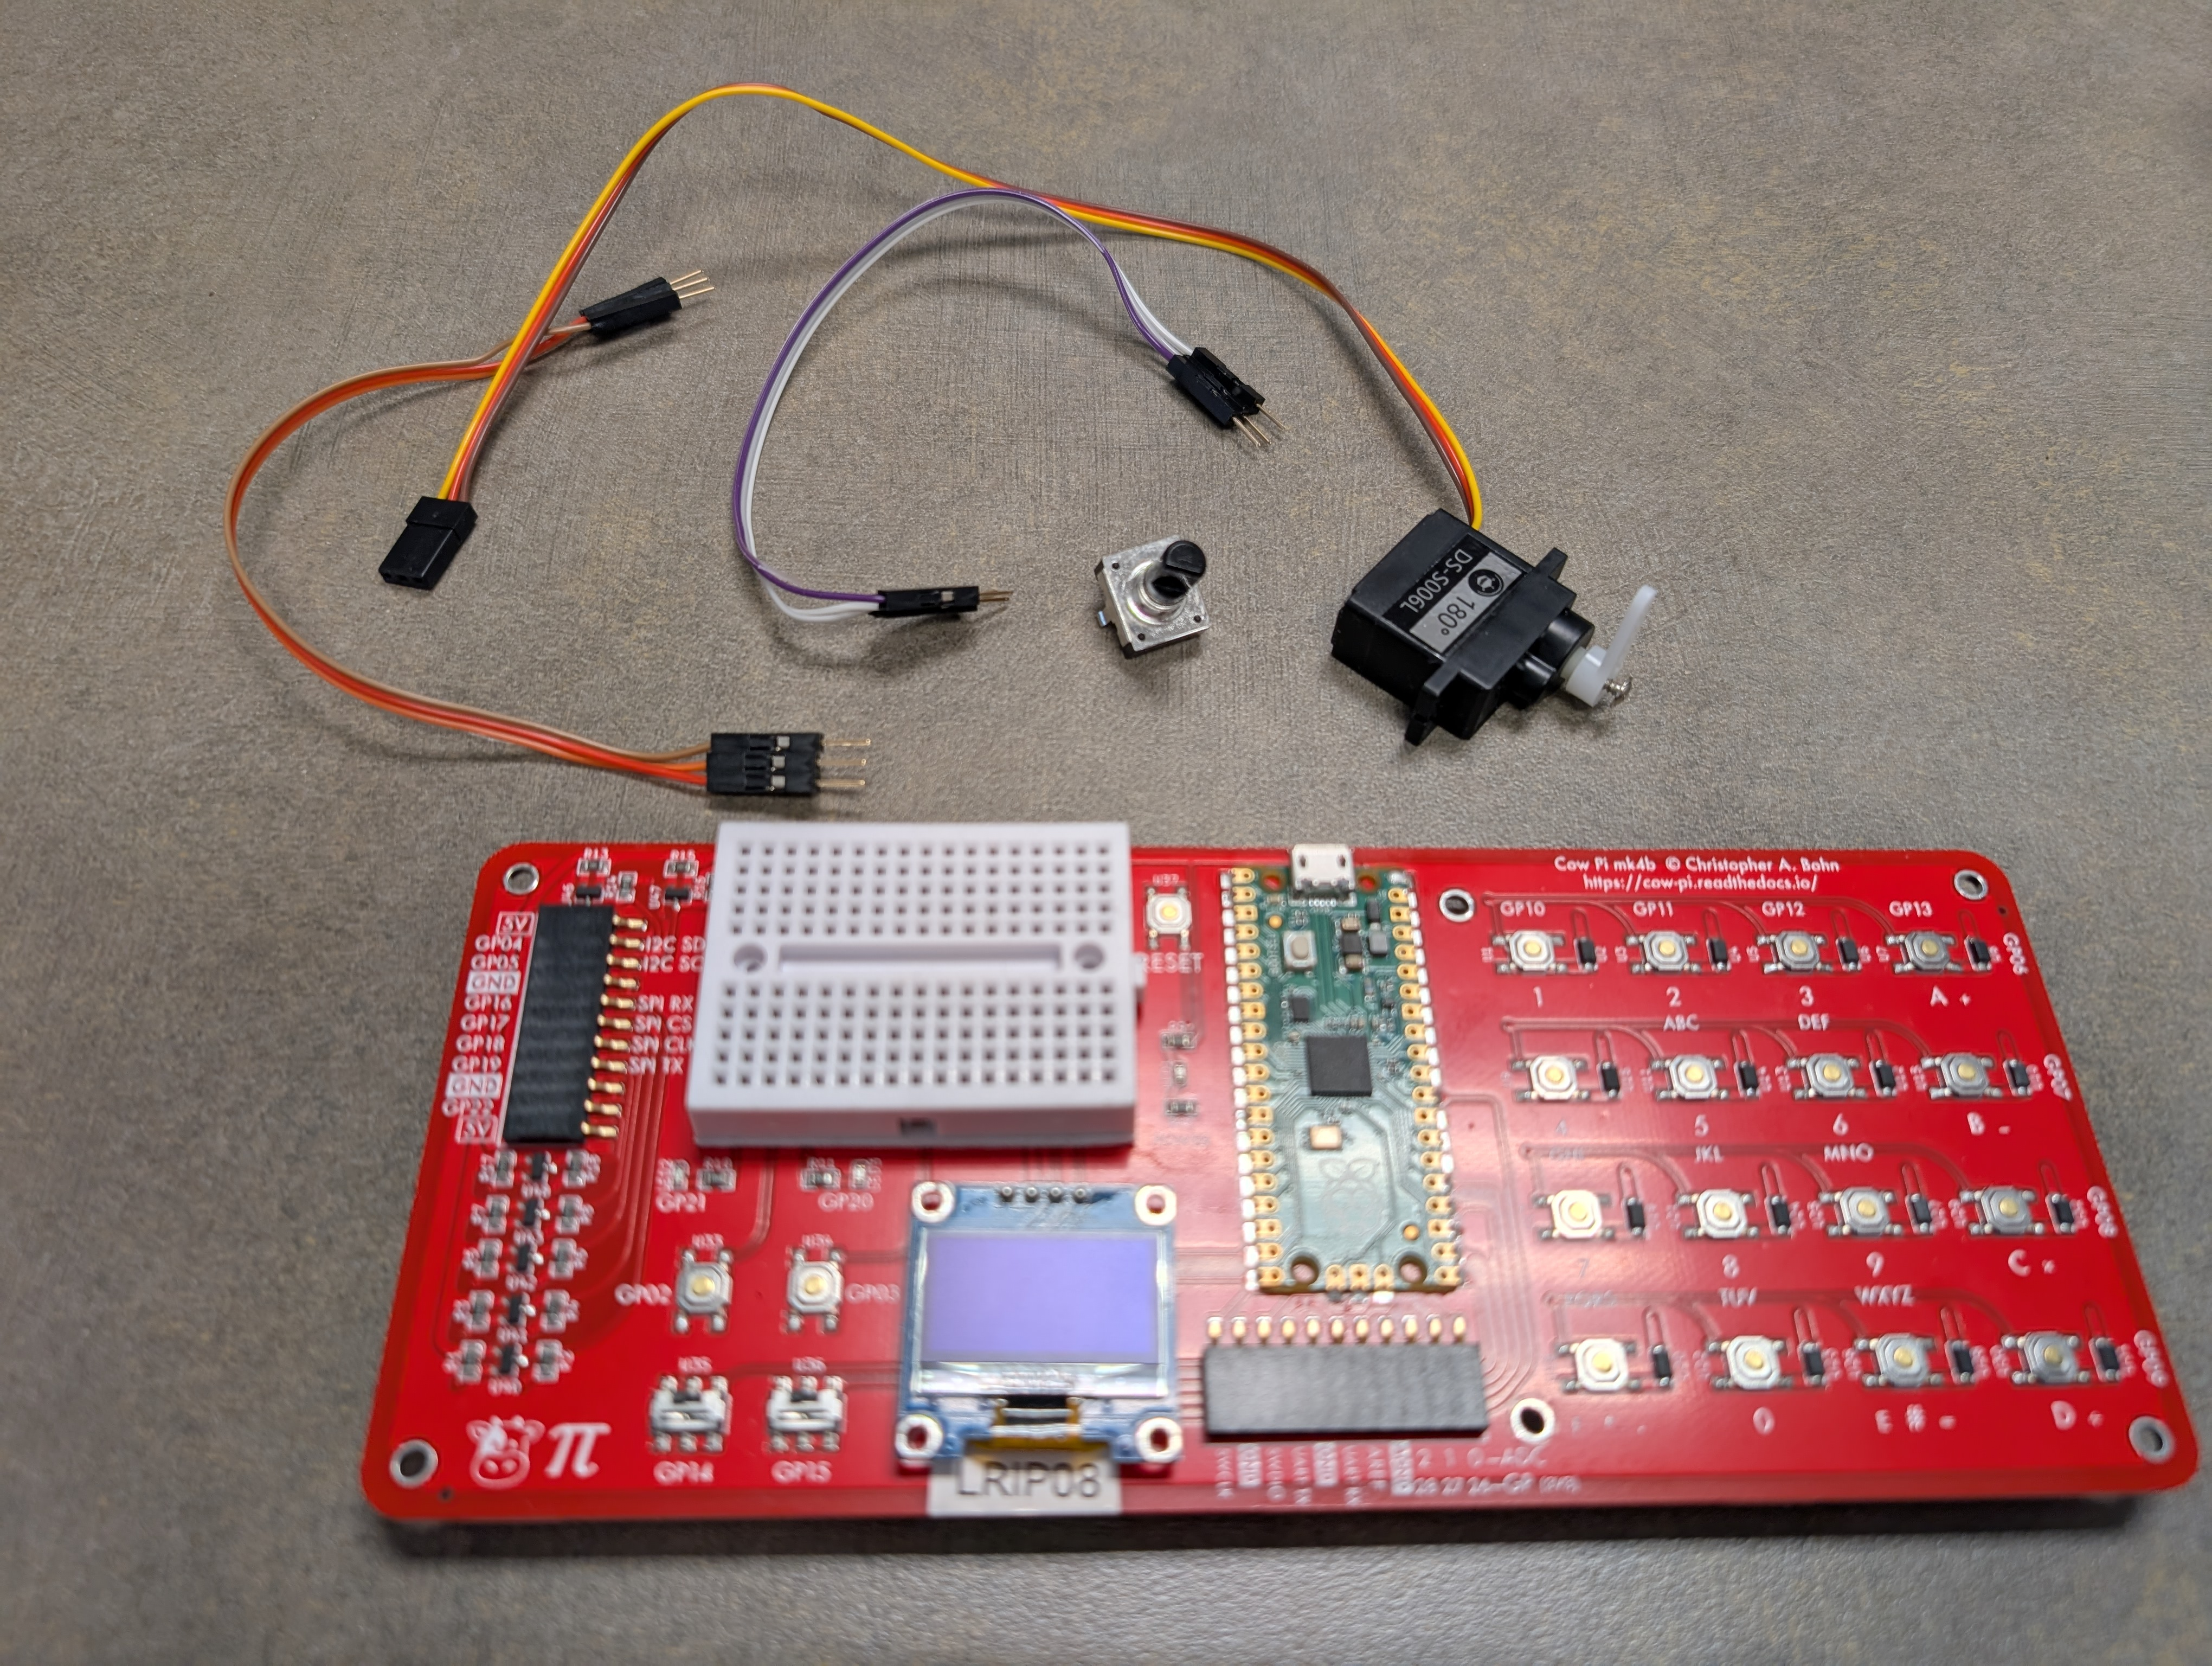
\includegraphics[width=10cm]{hardware/components}
    \caption{Components needed for the Range Finder \label{fig:components-mk4b}}
\end{figure}

You will need:
\begin{itemize}
    \item Your Cow Pi hardware circuit
    \item A rotary encoder
    \item A servomotor
    \item Six 20cm male-to-male wires
\end{itemize}

There is a labeled header on the left side of the Cow~Pi;
we will use this to connect the hardware components to the RP2040 microcontroller.

\subsection{The Mini-Breadboard on the Cow Pi}

A key feature of solderless breadboards, such as the mini-breadboard on your Cow~Pi, are the groups of 5 holes (Figure~\ref{fig:breadboard-mk4b}).
Each group of five is a \textit{terminal strip}.

\begin{figure}
    \centering
    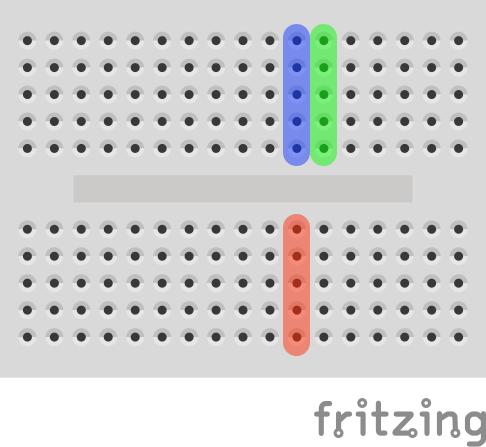
\includegraphics[height=4cm]{hardware/breadboard}
    \caption{Terminal strips on a mini-breadboard \label{fig:breadboard-mk4b}}
\end{figure}

The five holes in a terminal strip are electrically connected to each other but are electrically isolated from the other terminal strips.\footnote{
    They are isolated for DC signals, and parasitic reactance is negligible for AC signals below about 10~kHz.
}
For example, in Figure~\ref{fig:breadboard-mk4b}, all holes in the terminal strip that is highlighted in blue are connected to each other,
but they are not connected to the holes in the adjacent terminal strip highlighted in green.
Similarly, they are not connected to the holes in the red terminal strip on the other side of the gutter.

A consequence of this is that any components' connectors that are inserted into a terminal strip are connected to the connectors of other components that are inserted into the same terminal strip.

If you want to learn more, a very good overview of solderless breadboards can be found here: \url{https://learn.adafruit.com/breadboards-for-beginners?view=all}

%Figure~\ref{fig:breadboard-with-components-mk4b} shows where you will insert the hardware components for the group project.
%(The precise placement is not critical, so long as you make a note of which terminal strips you use.)
%
%\begin{figure}
%    \centering
%    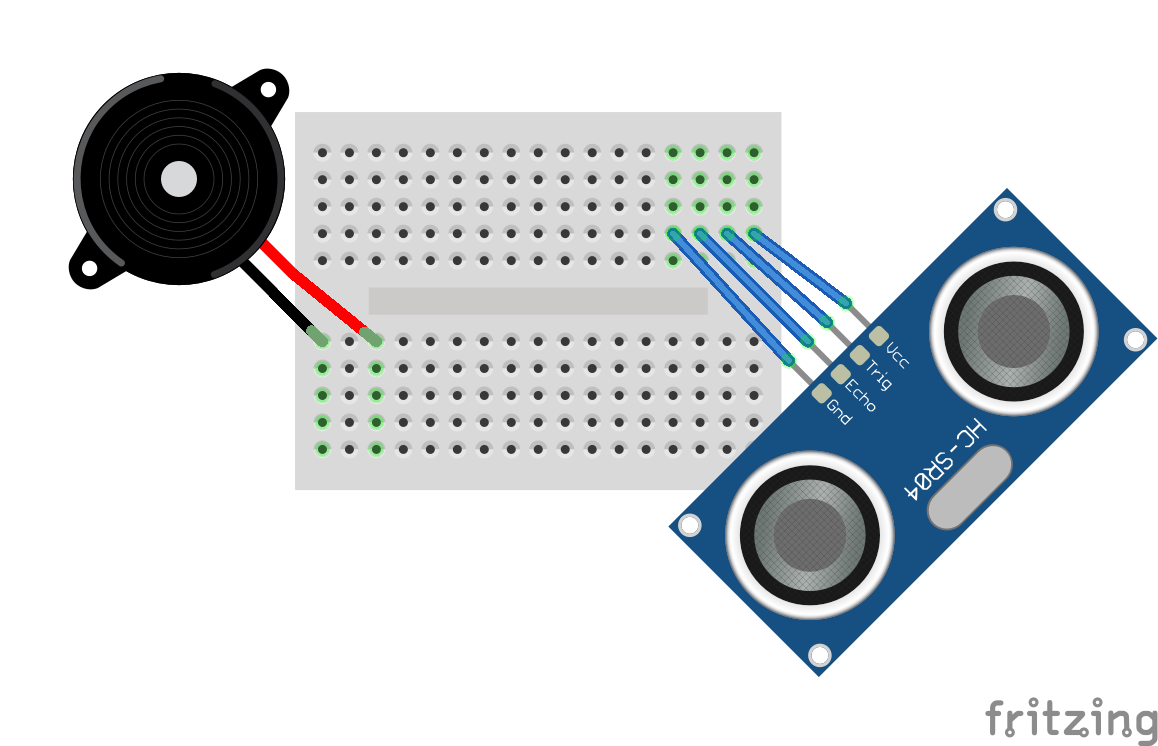
\includegraphics[height=4cm]{hardware/mk4b/breadboard-with-components}
%    \caption{Terminal strips on a mini-breadboard \label{fig:breadboard-with-components-mk4b}}
%\end{figure}


\subsection{Connecting the servomotor}

If your servomotor does not already have a servo arm attached, attach a servo arm to the motor's shaft.
See Figure~\ref{fig:servoArm}.
The orientation does not matter since we will not connect anything to the servo -- we are simply using the servomotor to simulate a lock's deadbolt mechanism,
and the arm will allow us to see the motion.
\textit{Do \underline{not} screw the arm to the motor's shaft.}
Simply let it fit snugly.


\begin{figure}
    \centering
    \subfloat[A servo arm can be attached to a servo motor.]{
        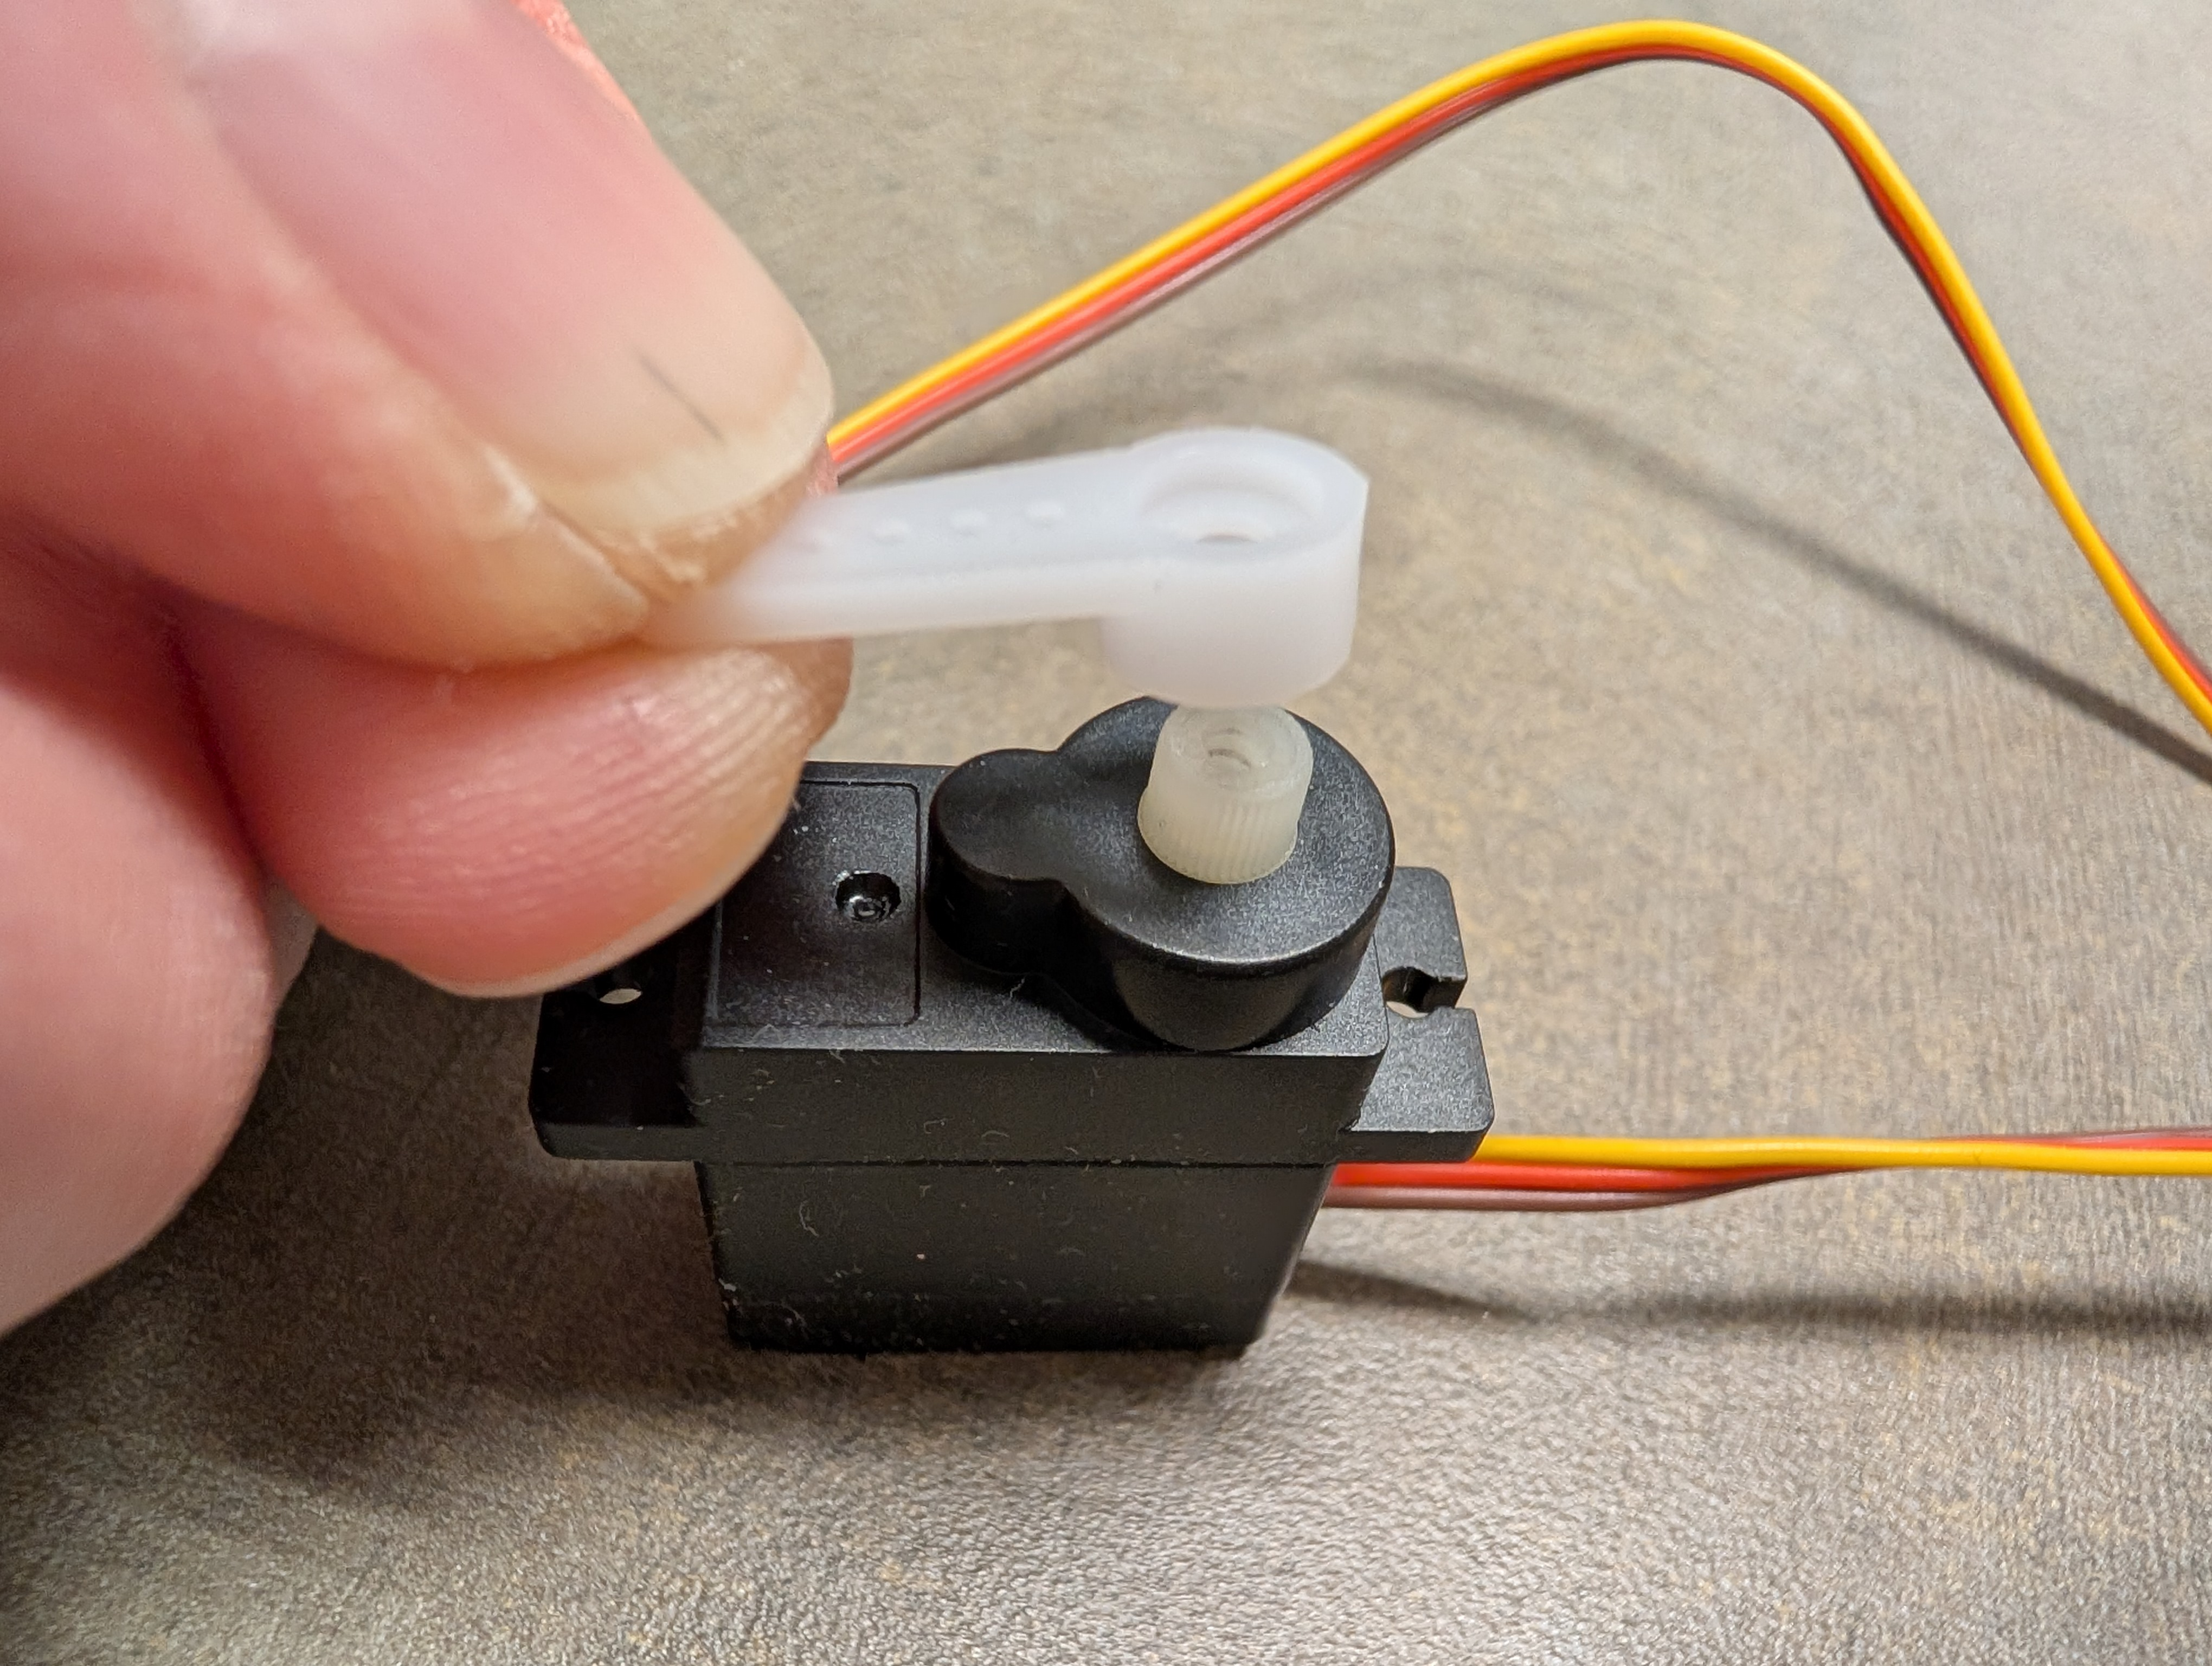
\includegraphics[height=4cm]{hardware/aboutToAttachServoArm}
%        \label{fig:attaching}
    }
    \hfil
    \subfloat[A servo arm has been attached to a servo motor.]{
        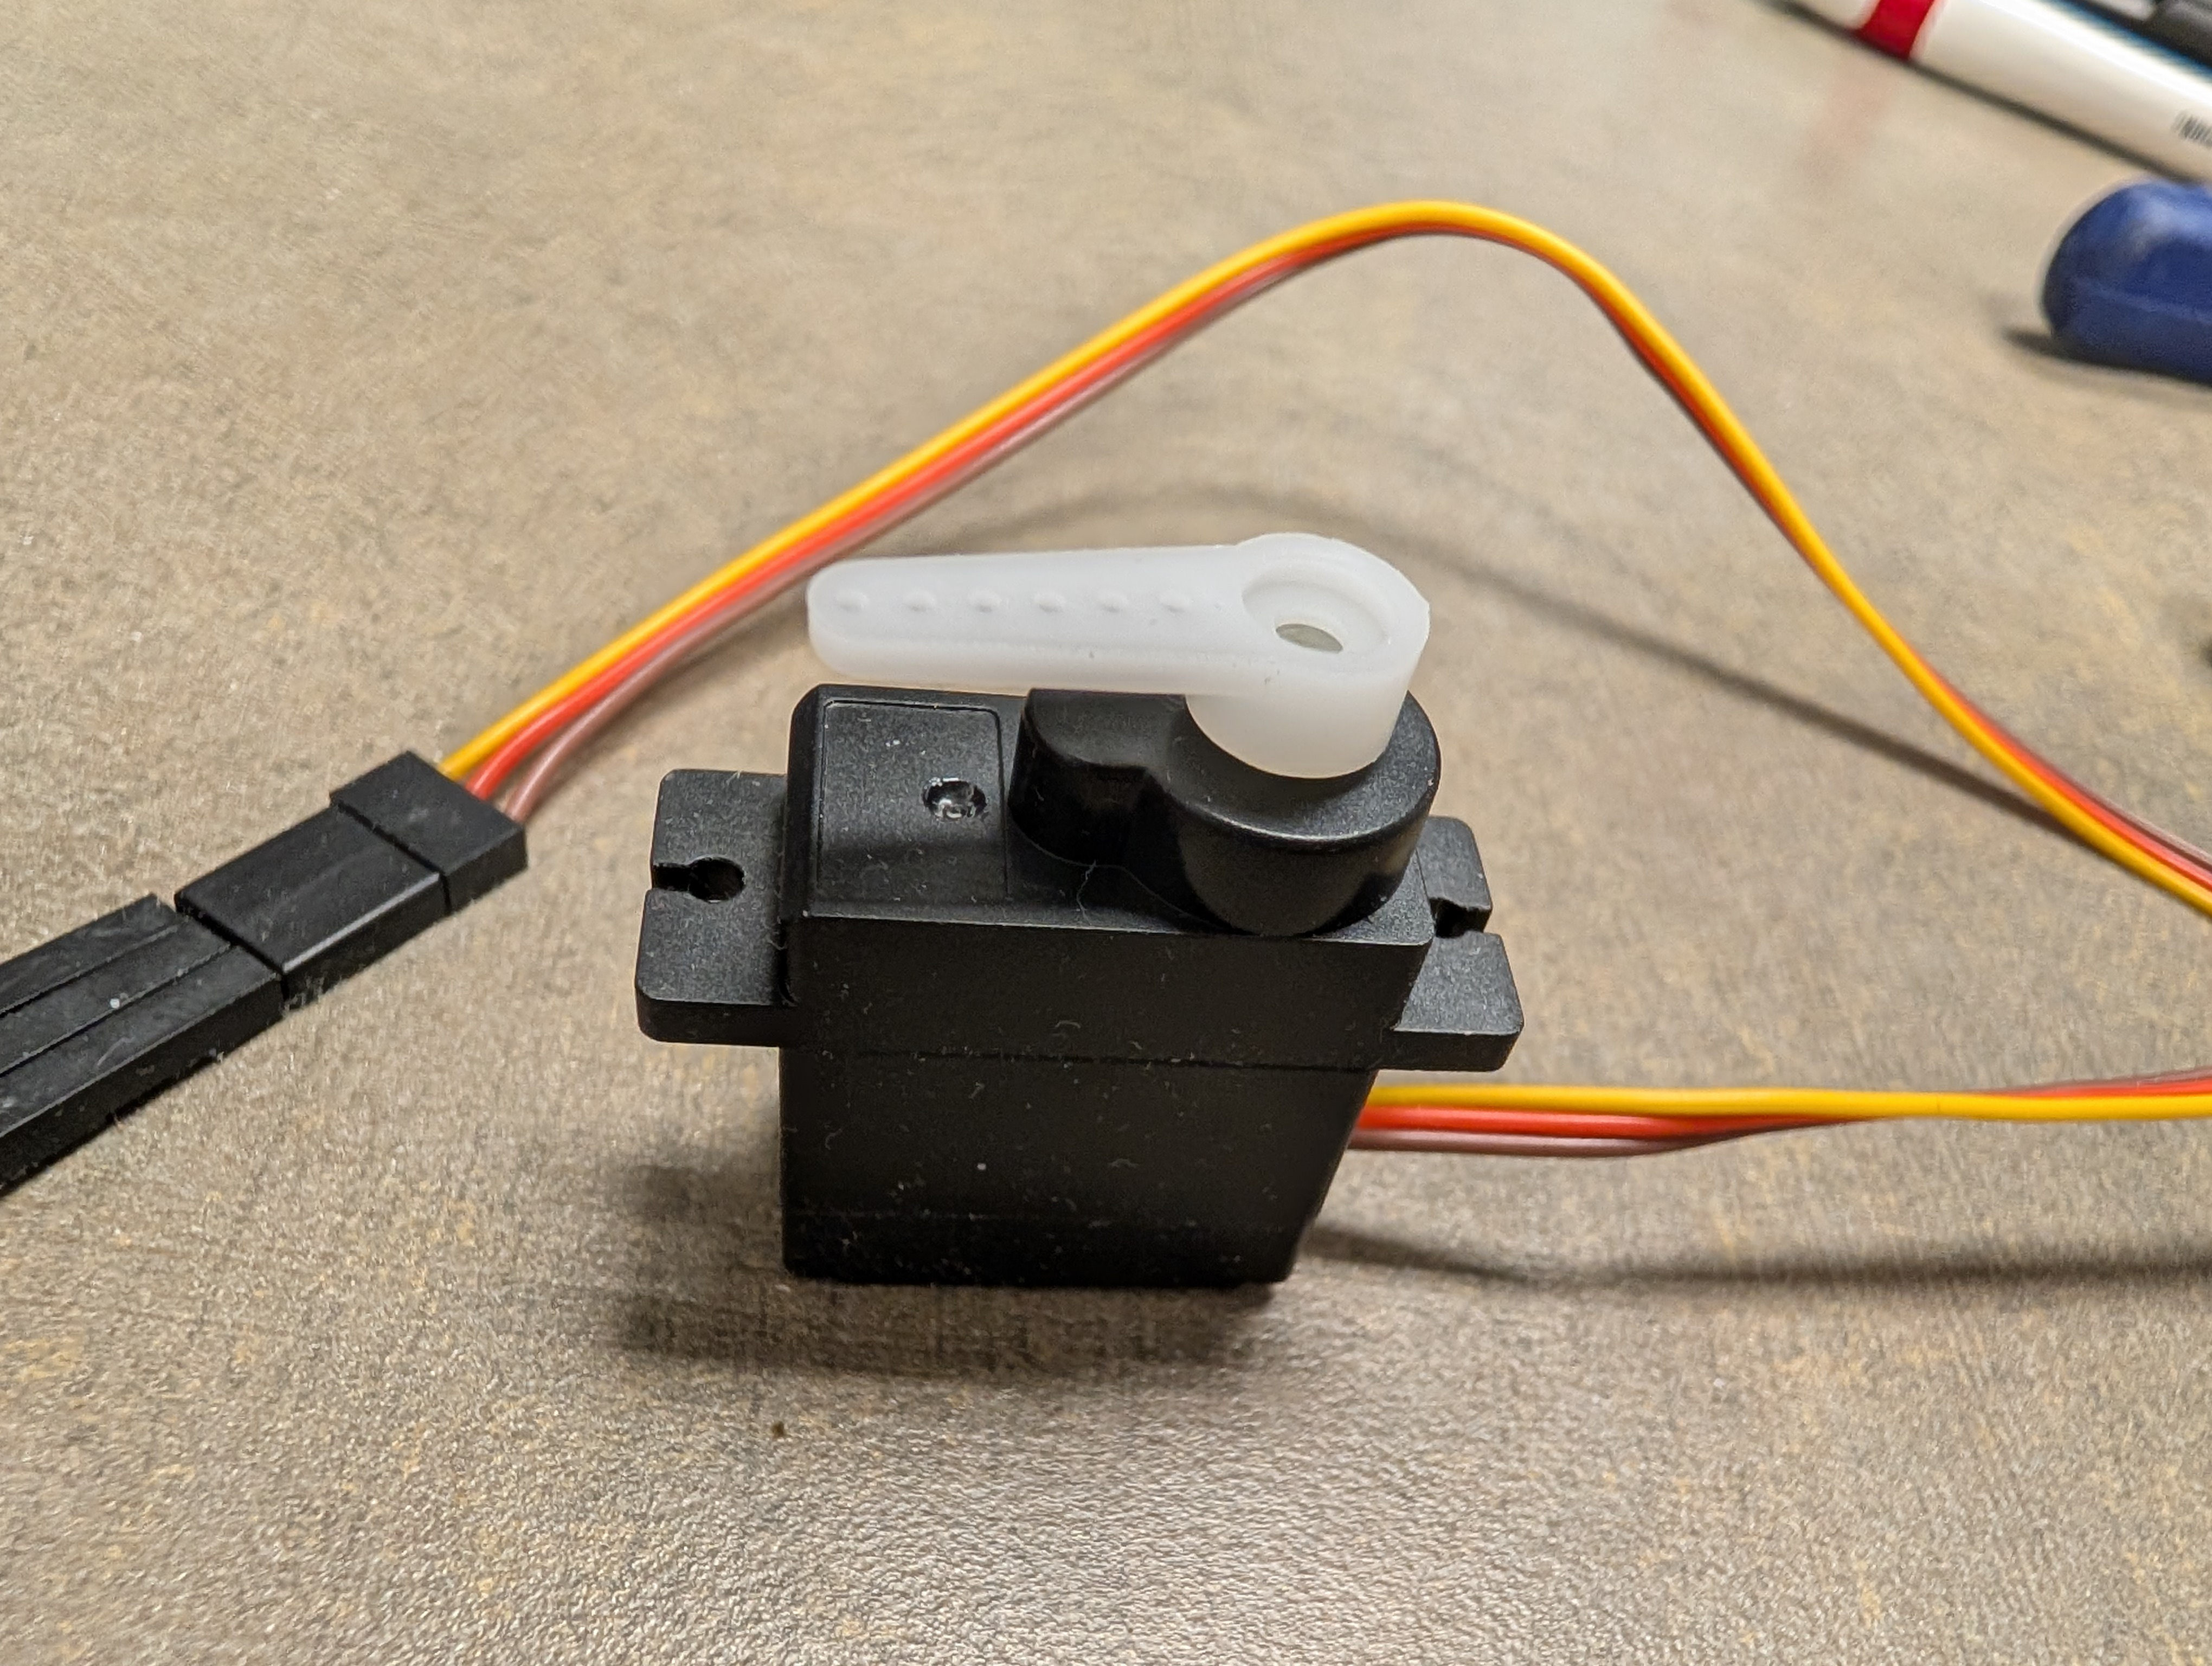
\includegraphics[height=4cm]{hardware/servoArmAttached}
%        \label{fig:attached}
    }
    \caption{Attaching a servo arm to a servo motor. \label{fig:servoArm}}
\end{figure}

\begin{description}
    \checkoffitem{Attach three to the servo's wires (Figure~\ref{fig:attachWiresToServo}).
        The colors do not need to match, but you do need to pay attention to which 20cm wire you attached to which servo wire.}
    \checkoffitem{Locate the 20cm that is attached to the servo's \textbf{red} wire. Insert the other end into a \texttt{5V} slot.}
    \checkoffitem{Locate the 20cm that is attached to the servo's \textbf{brown} wire. Insert the other end into a \texttt{GND} slot.}
    \checkoffitem{Locate the 20cm that is attached to the servo's \textbf{yelow} wire. Insert the other end into the \texttt{GP22} slot.}
    \checkoffitem{\textcolor{red}{Have someone verify that you have each wire inserted into the correct slot.}}
\end{description}


\begin{figure}
    \centering
    \subfloat[Attaching 20cm wires to servo wires.]{
        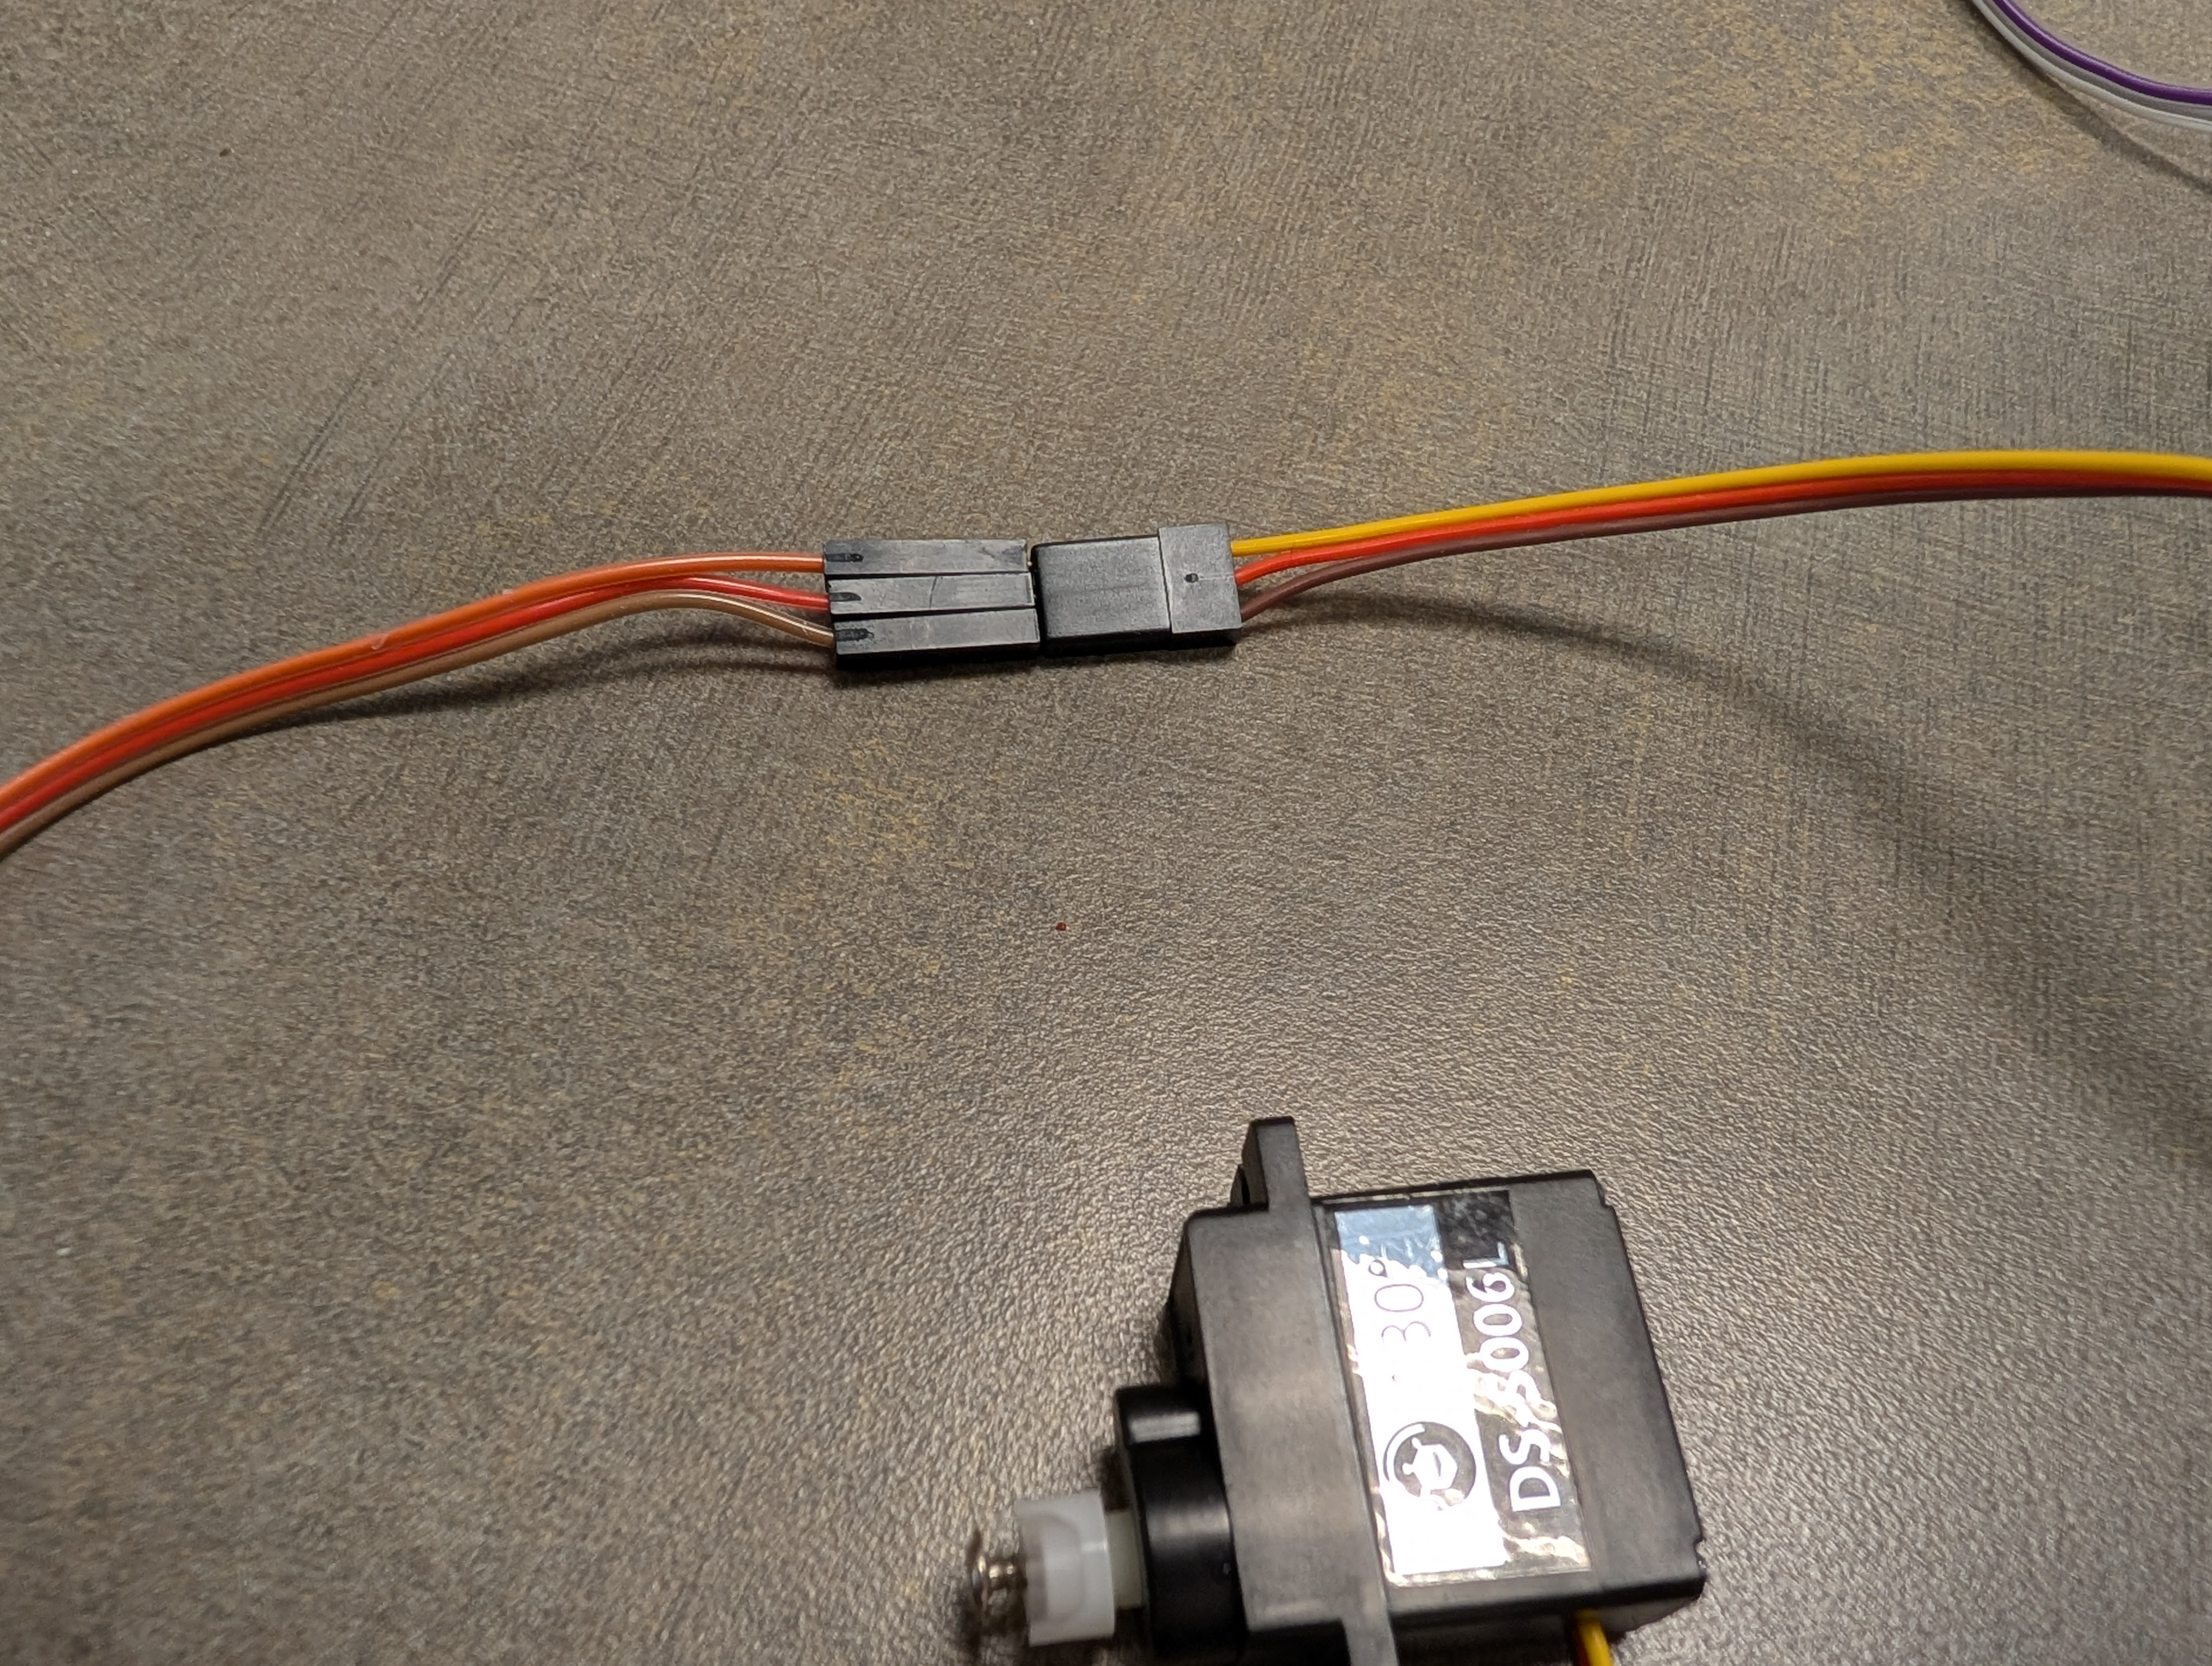
\includegraphics[height=4cm]{hardware/attachWiresToServo}
        \label{fig:attachWiresToServo}
    }
    \\
    \subfloat[Determining where to insert each wire.]{
        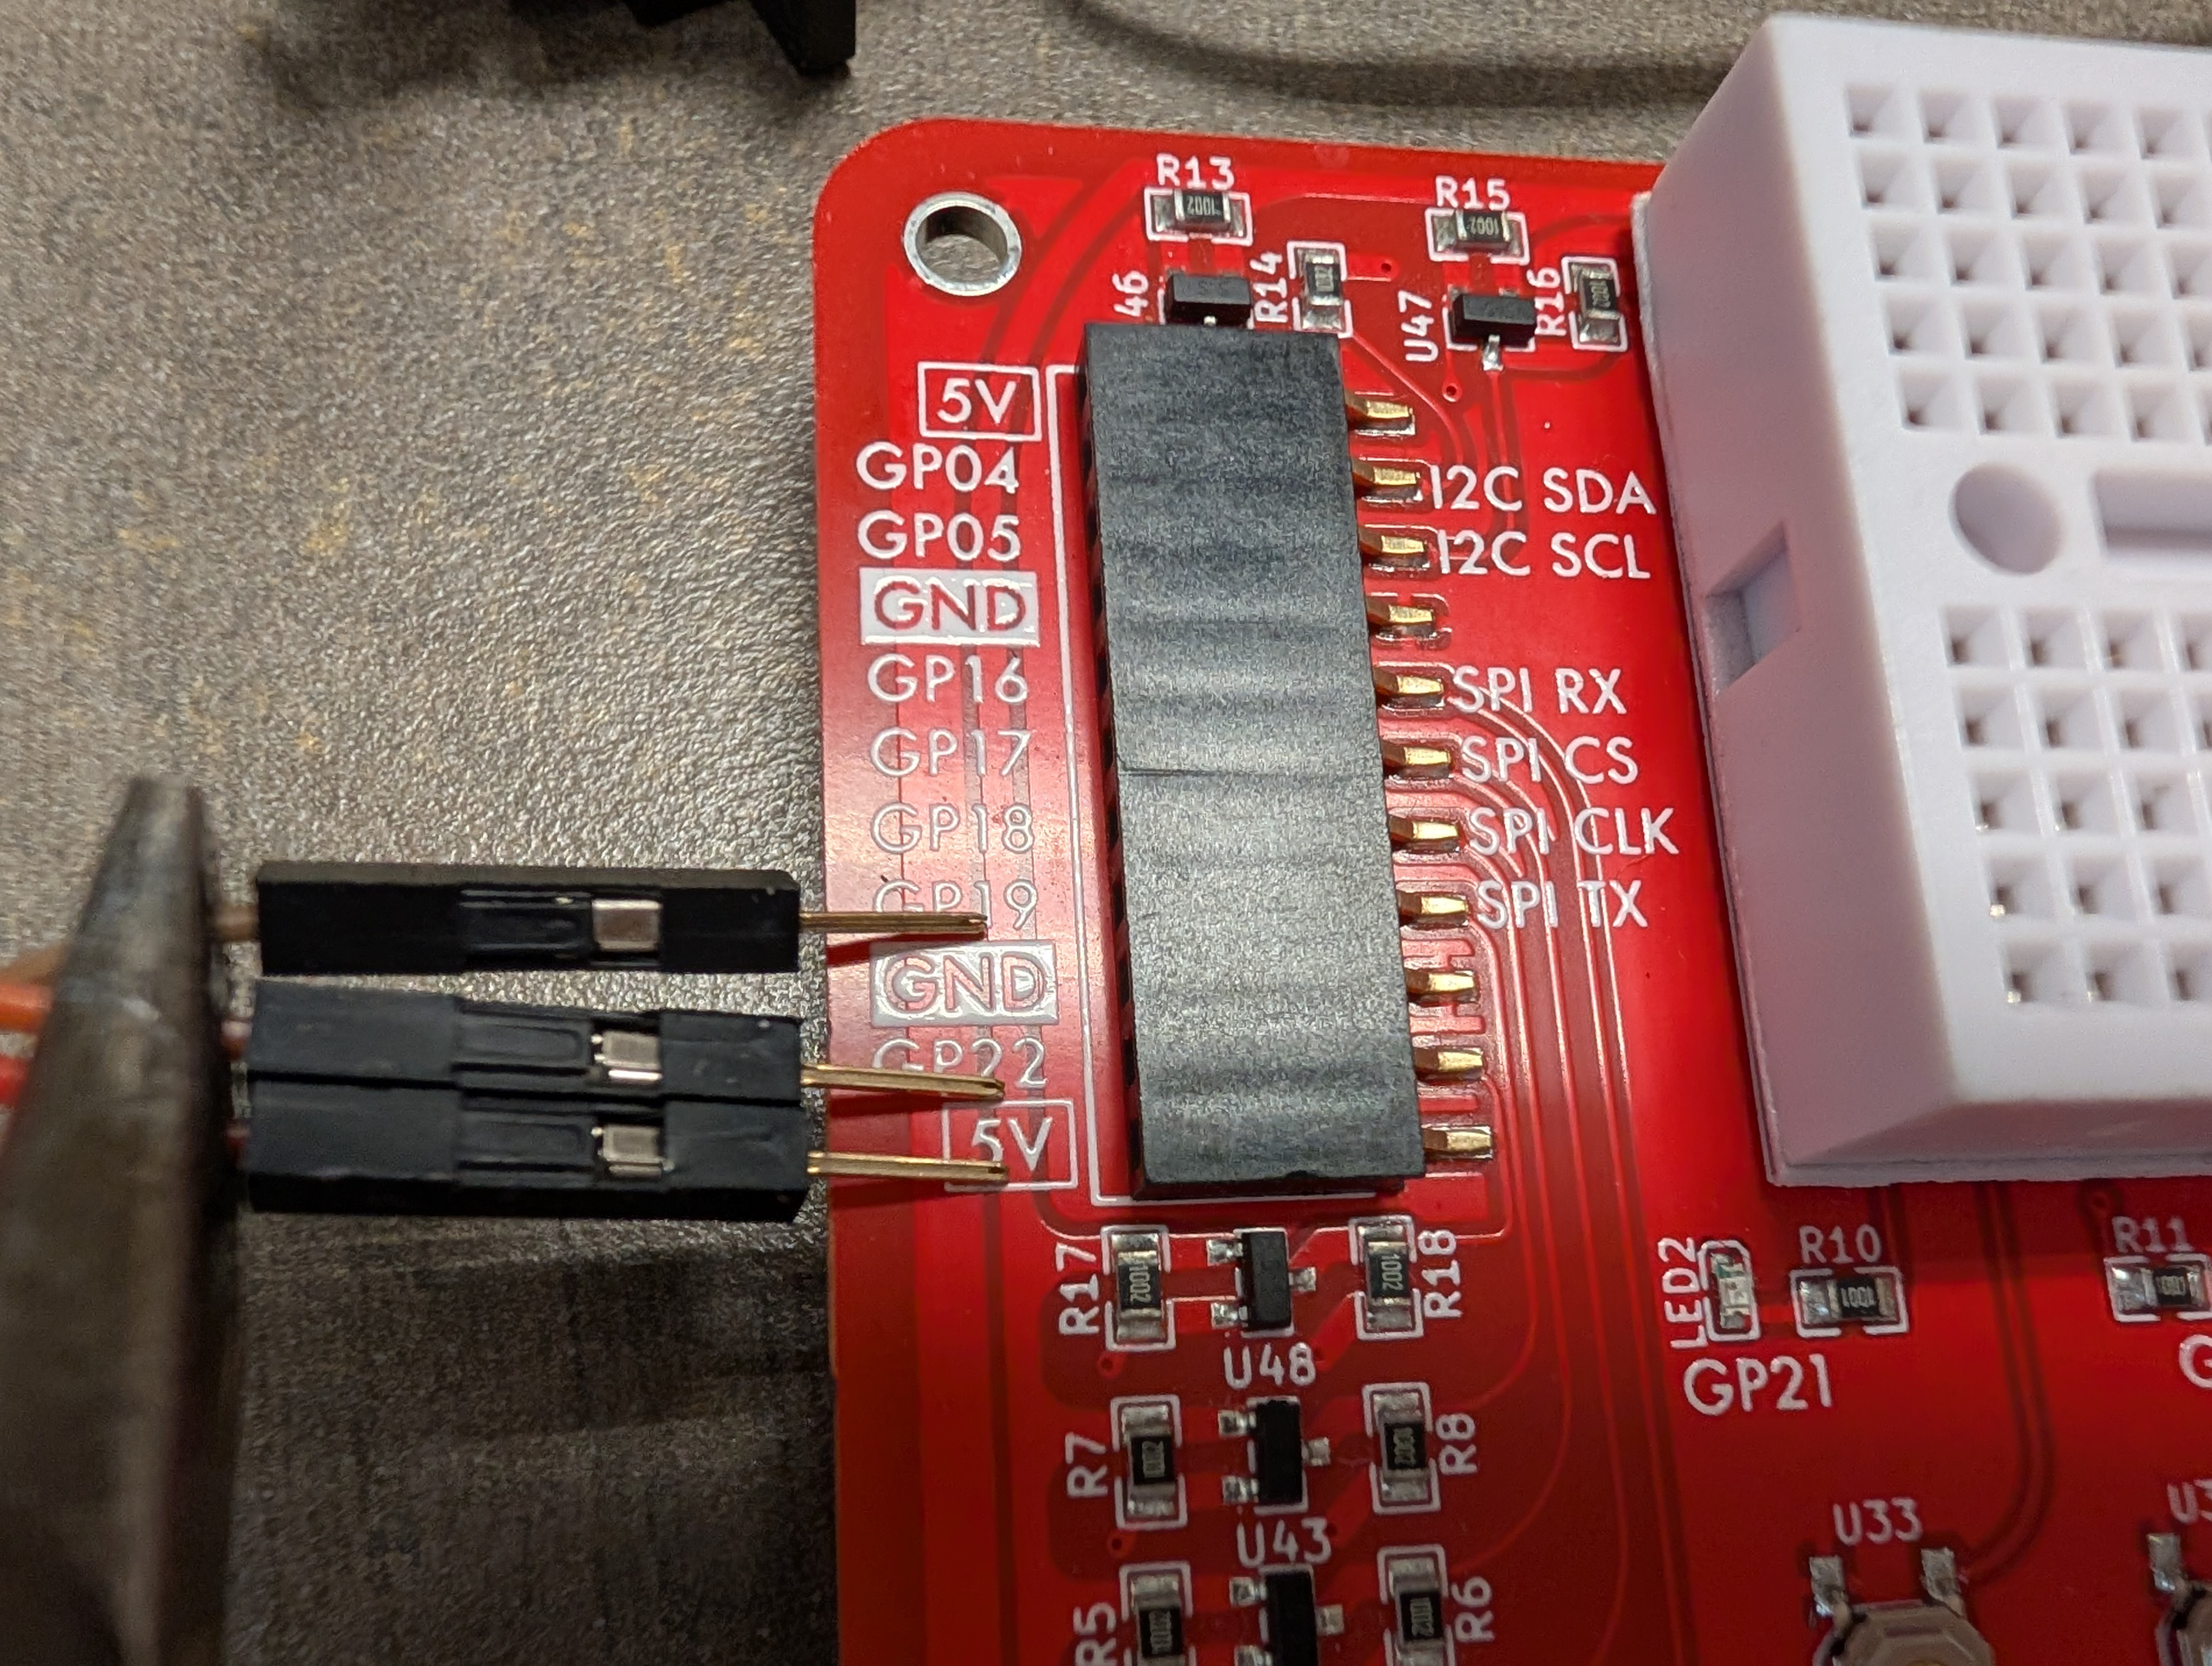
\includegraphics[height=4cm]{hardware/attachingServo}
%        \label{fig:attached}
    }
    \hfil
    \subfloat[All servo wires connected.]{
        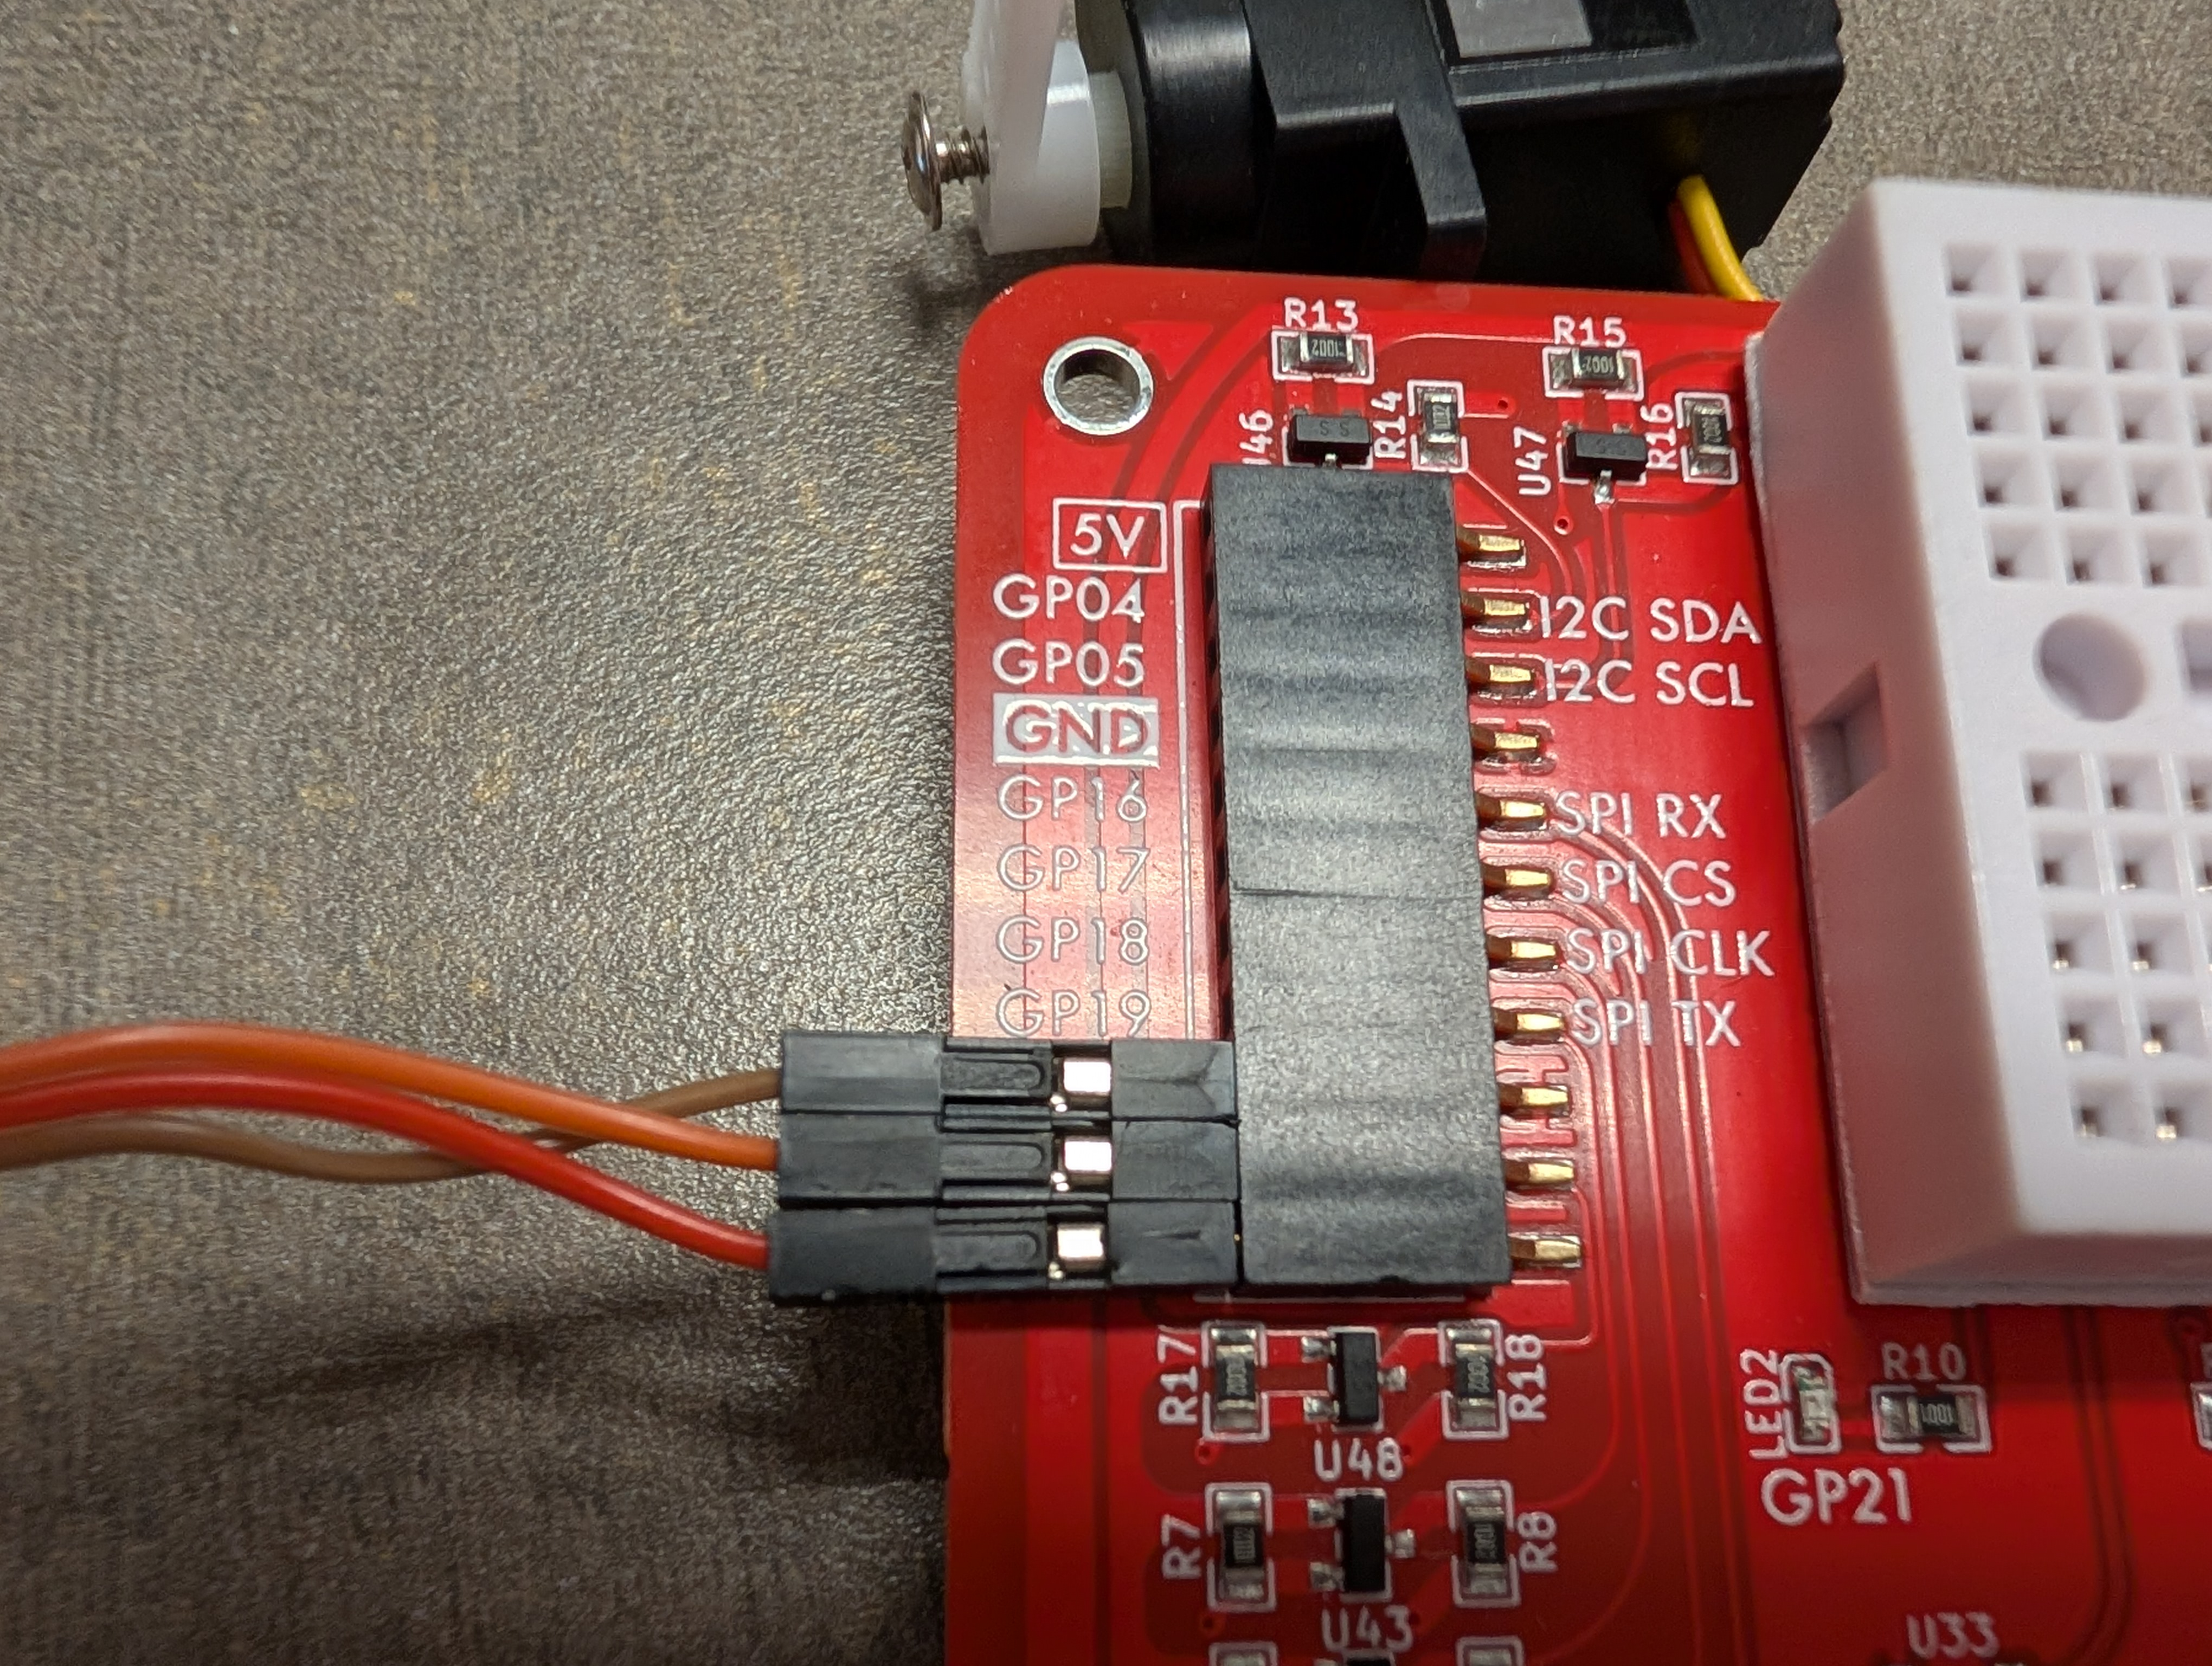
\includegraphics[height=4cm]{hardware/servoAttached}
%        \label{fig:attached}
    }
    \caption{Wiring a servo motor to the Cow~Pi. \label{fig:servoWiring}}
\end{figure}

The servo motor is now connected to the Cow~Pi's \texttt{GP22} pin.
The starter code will configure \texttt{GP22} to be an output pin.


\subsection{Connecting the Rotary Encoder}

\begin{figure}
    \centering
    \subfloat[Position the prongs into the breadboard gutter.]{
        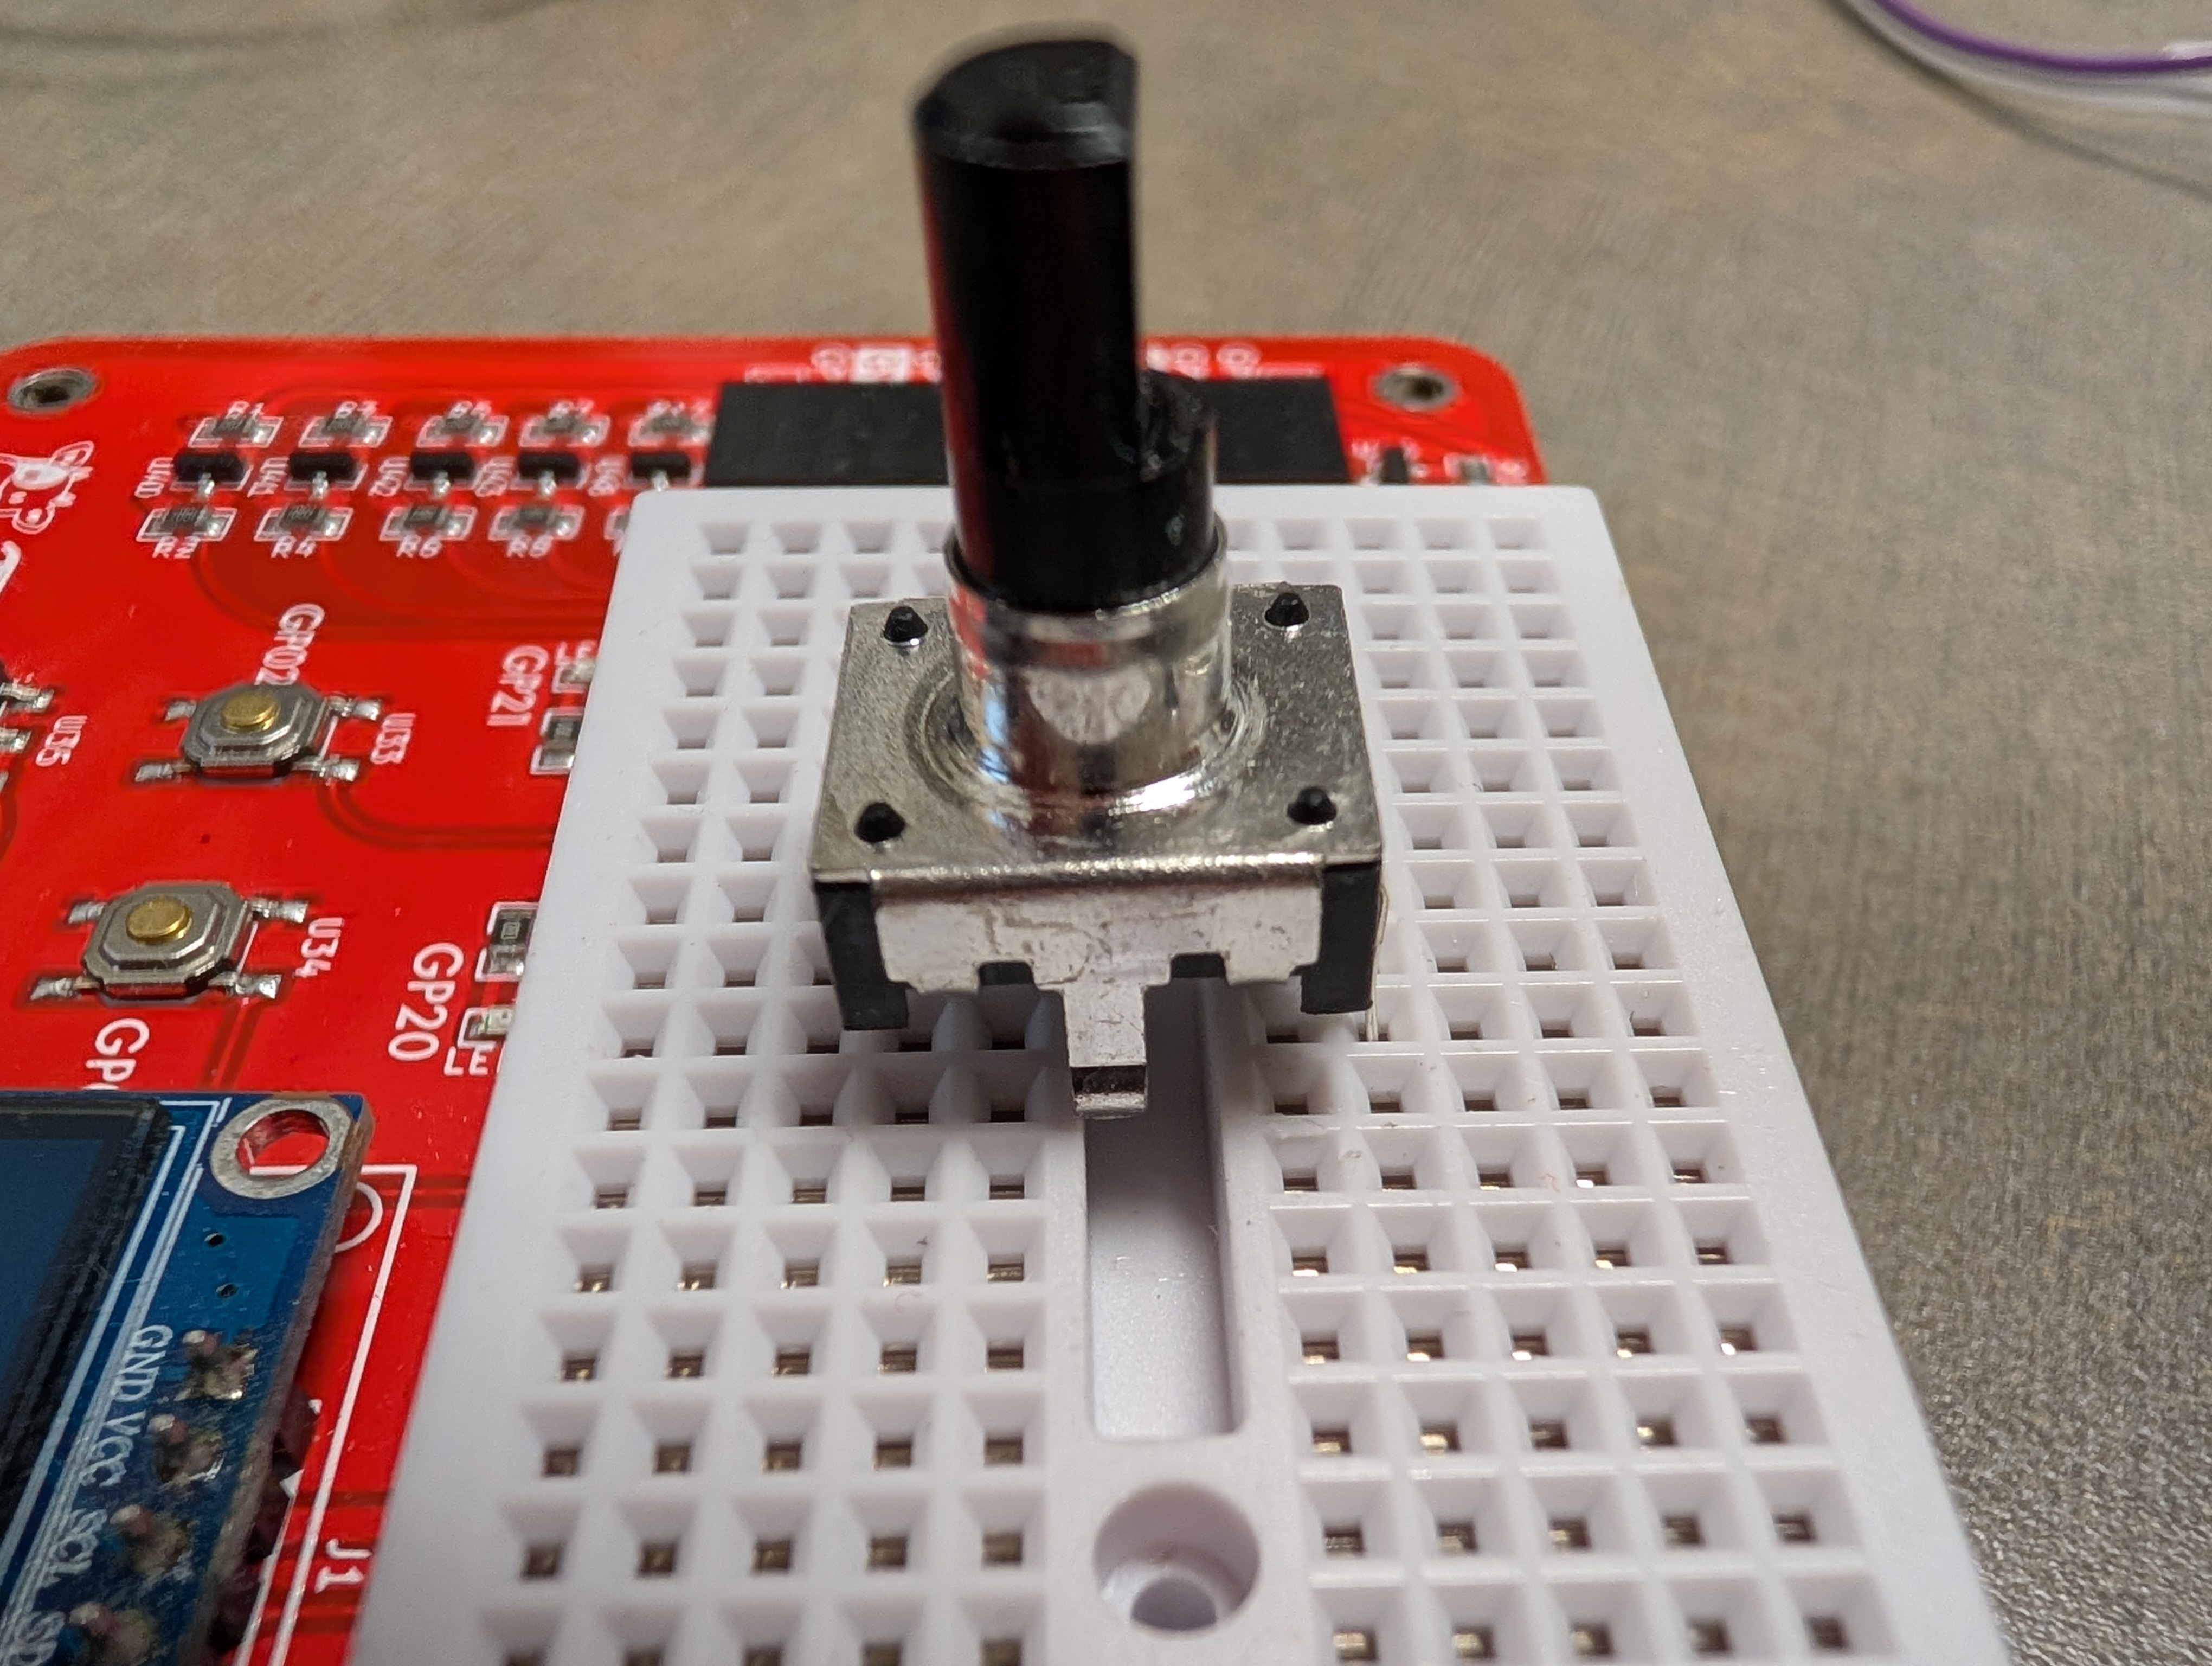
\includegraphics[height=4cm]{hardware/rotaryEncoderProngAlignment}
        \label{fig:rotaryEncoderProngs}
    }
    \hfil
    \subfloat[Placing the pins in contact point wells.]{
        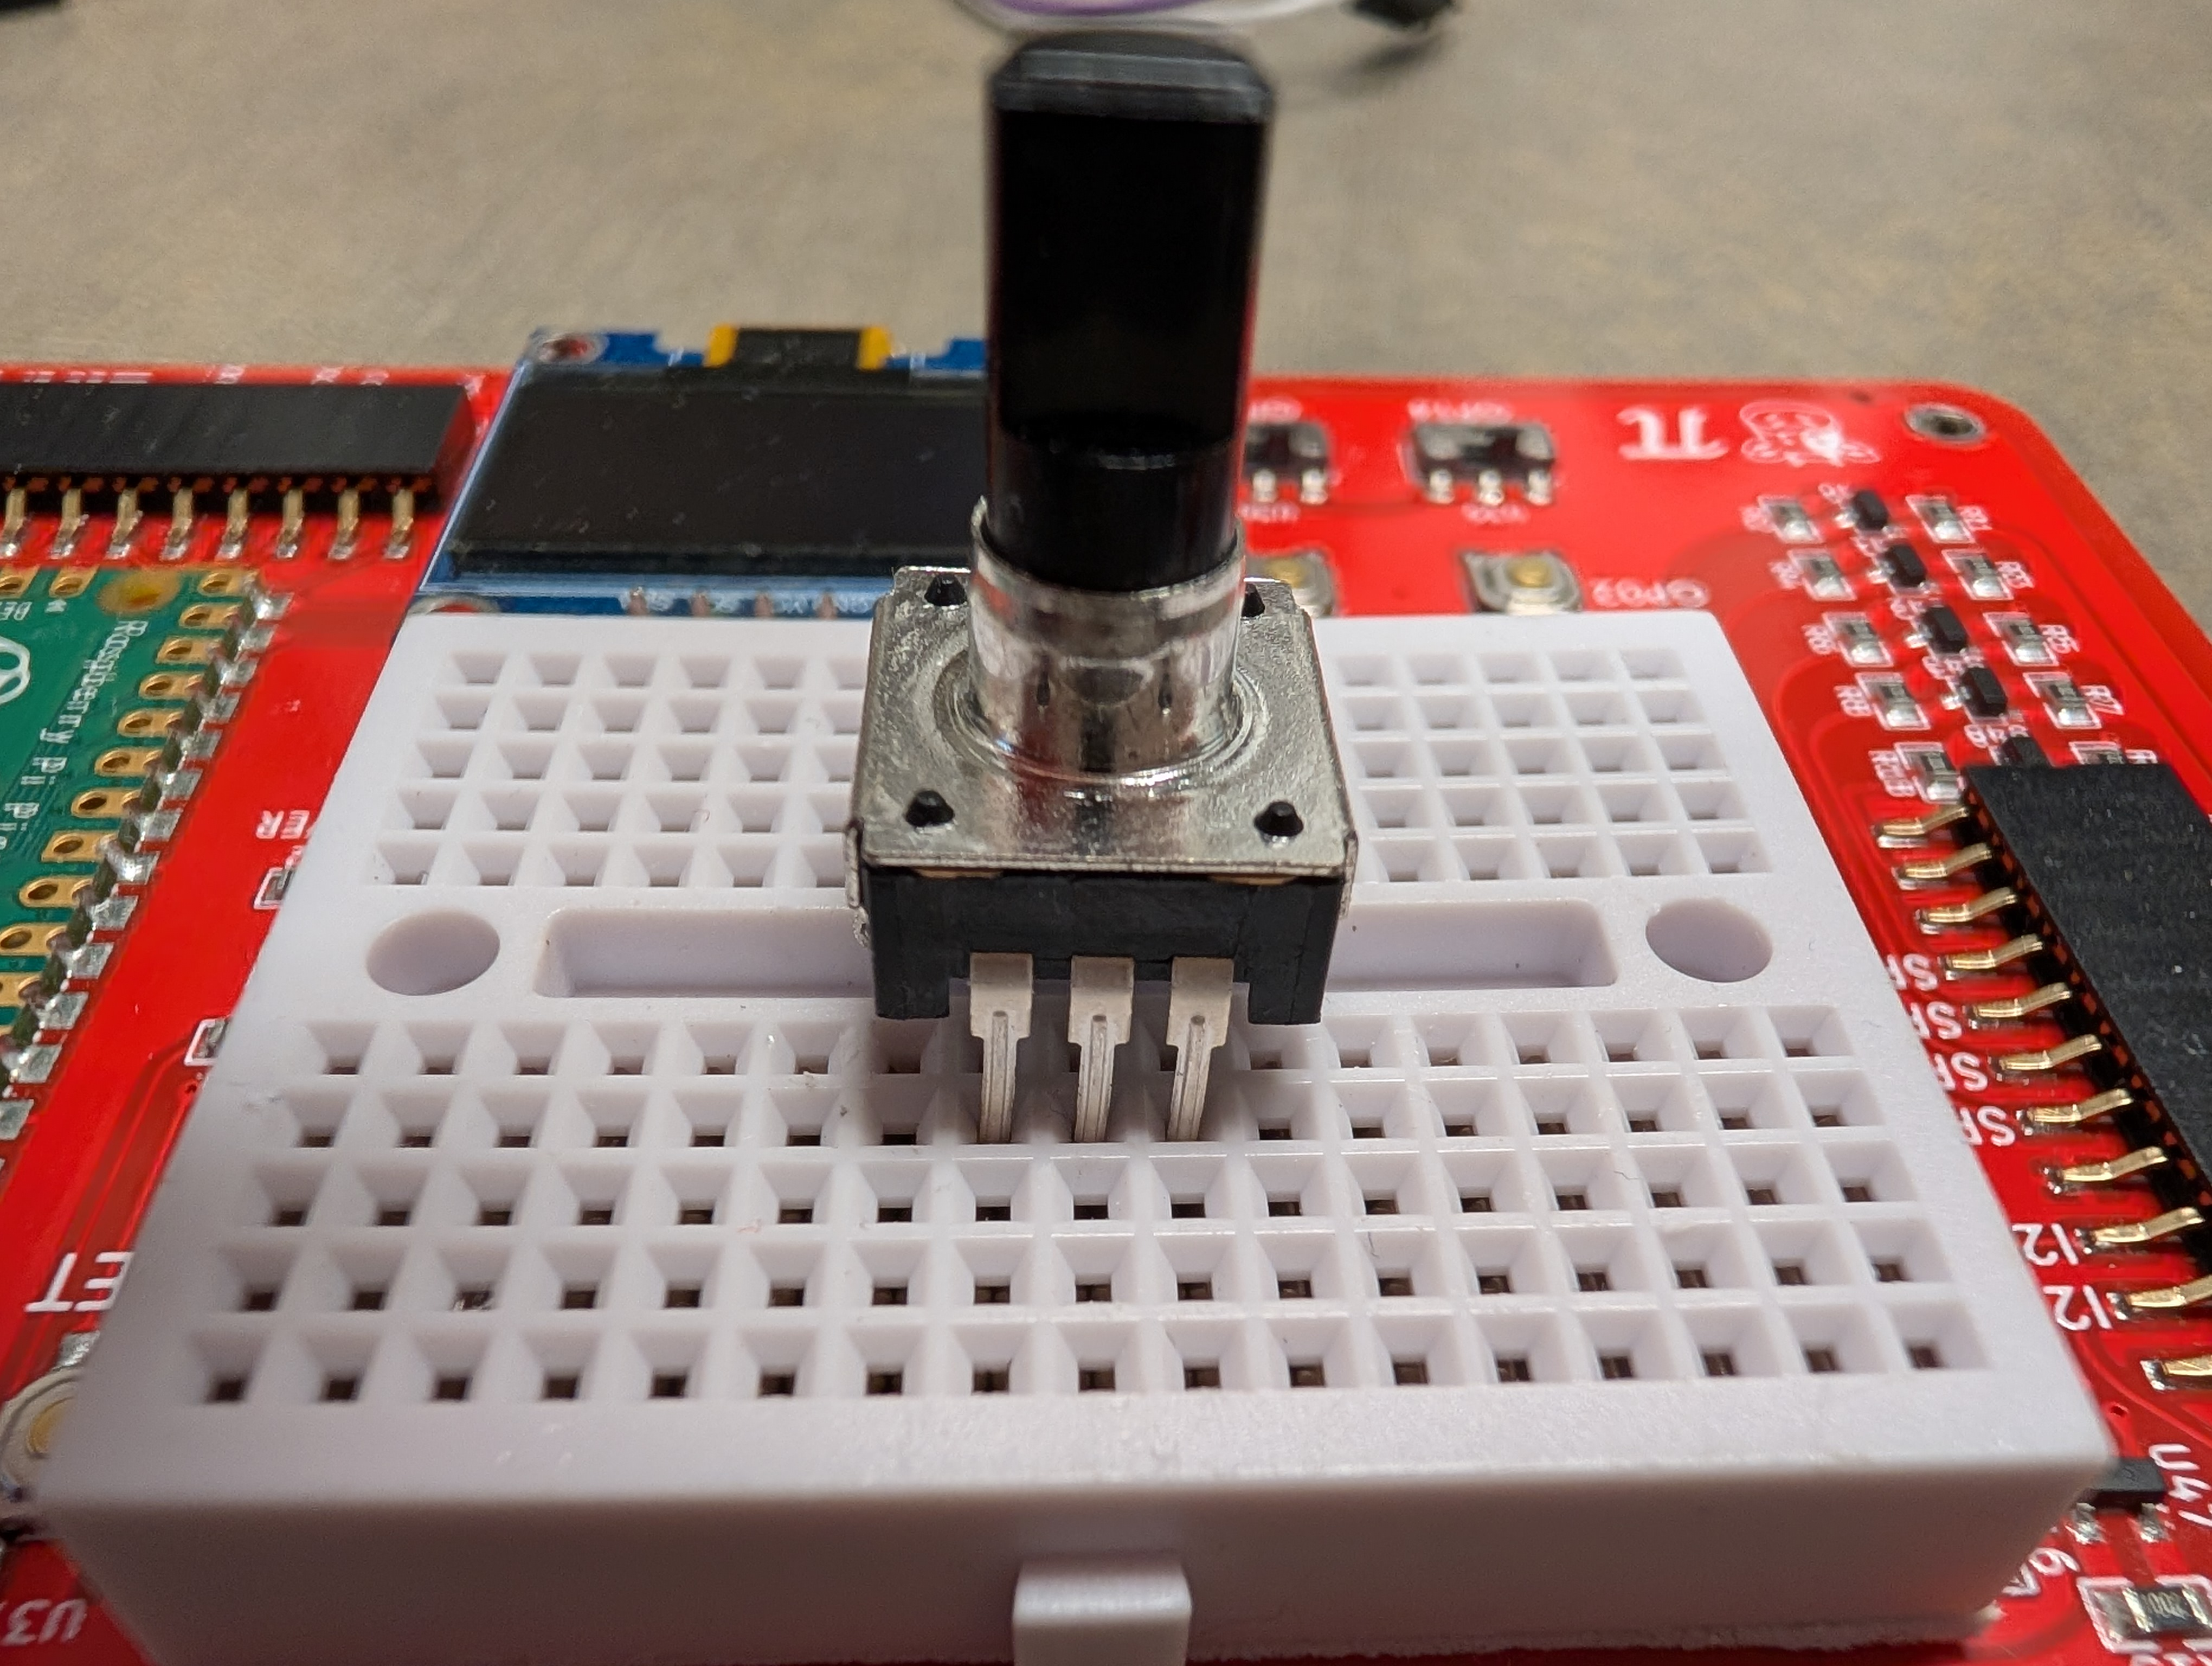
\includegraphics[height=4cm]{hardware/rotaryEncoderPins}
        \label{fig:rotaryEncoderPins}
    }
    \\
    \subfloat[The rotary encoder in the breadboard.]{
        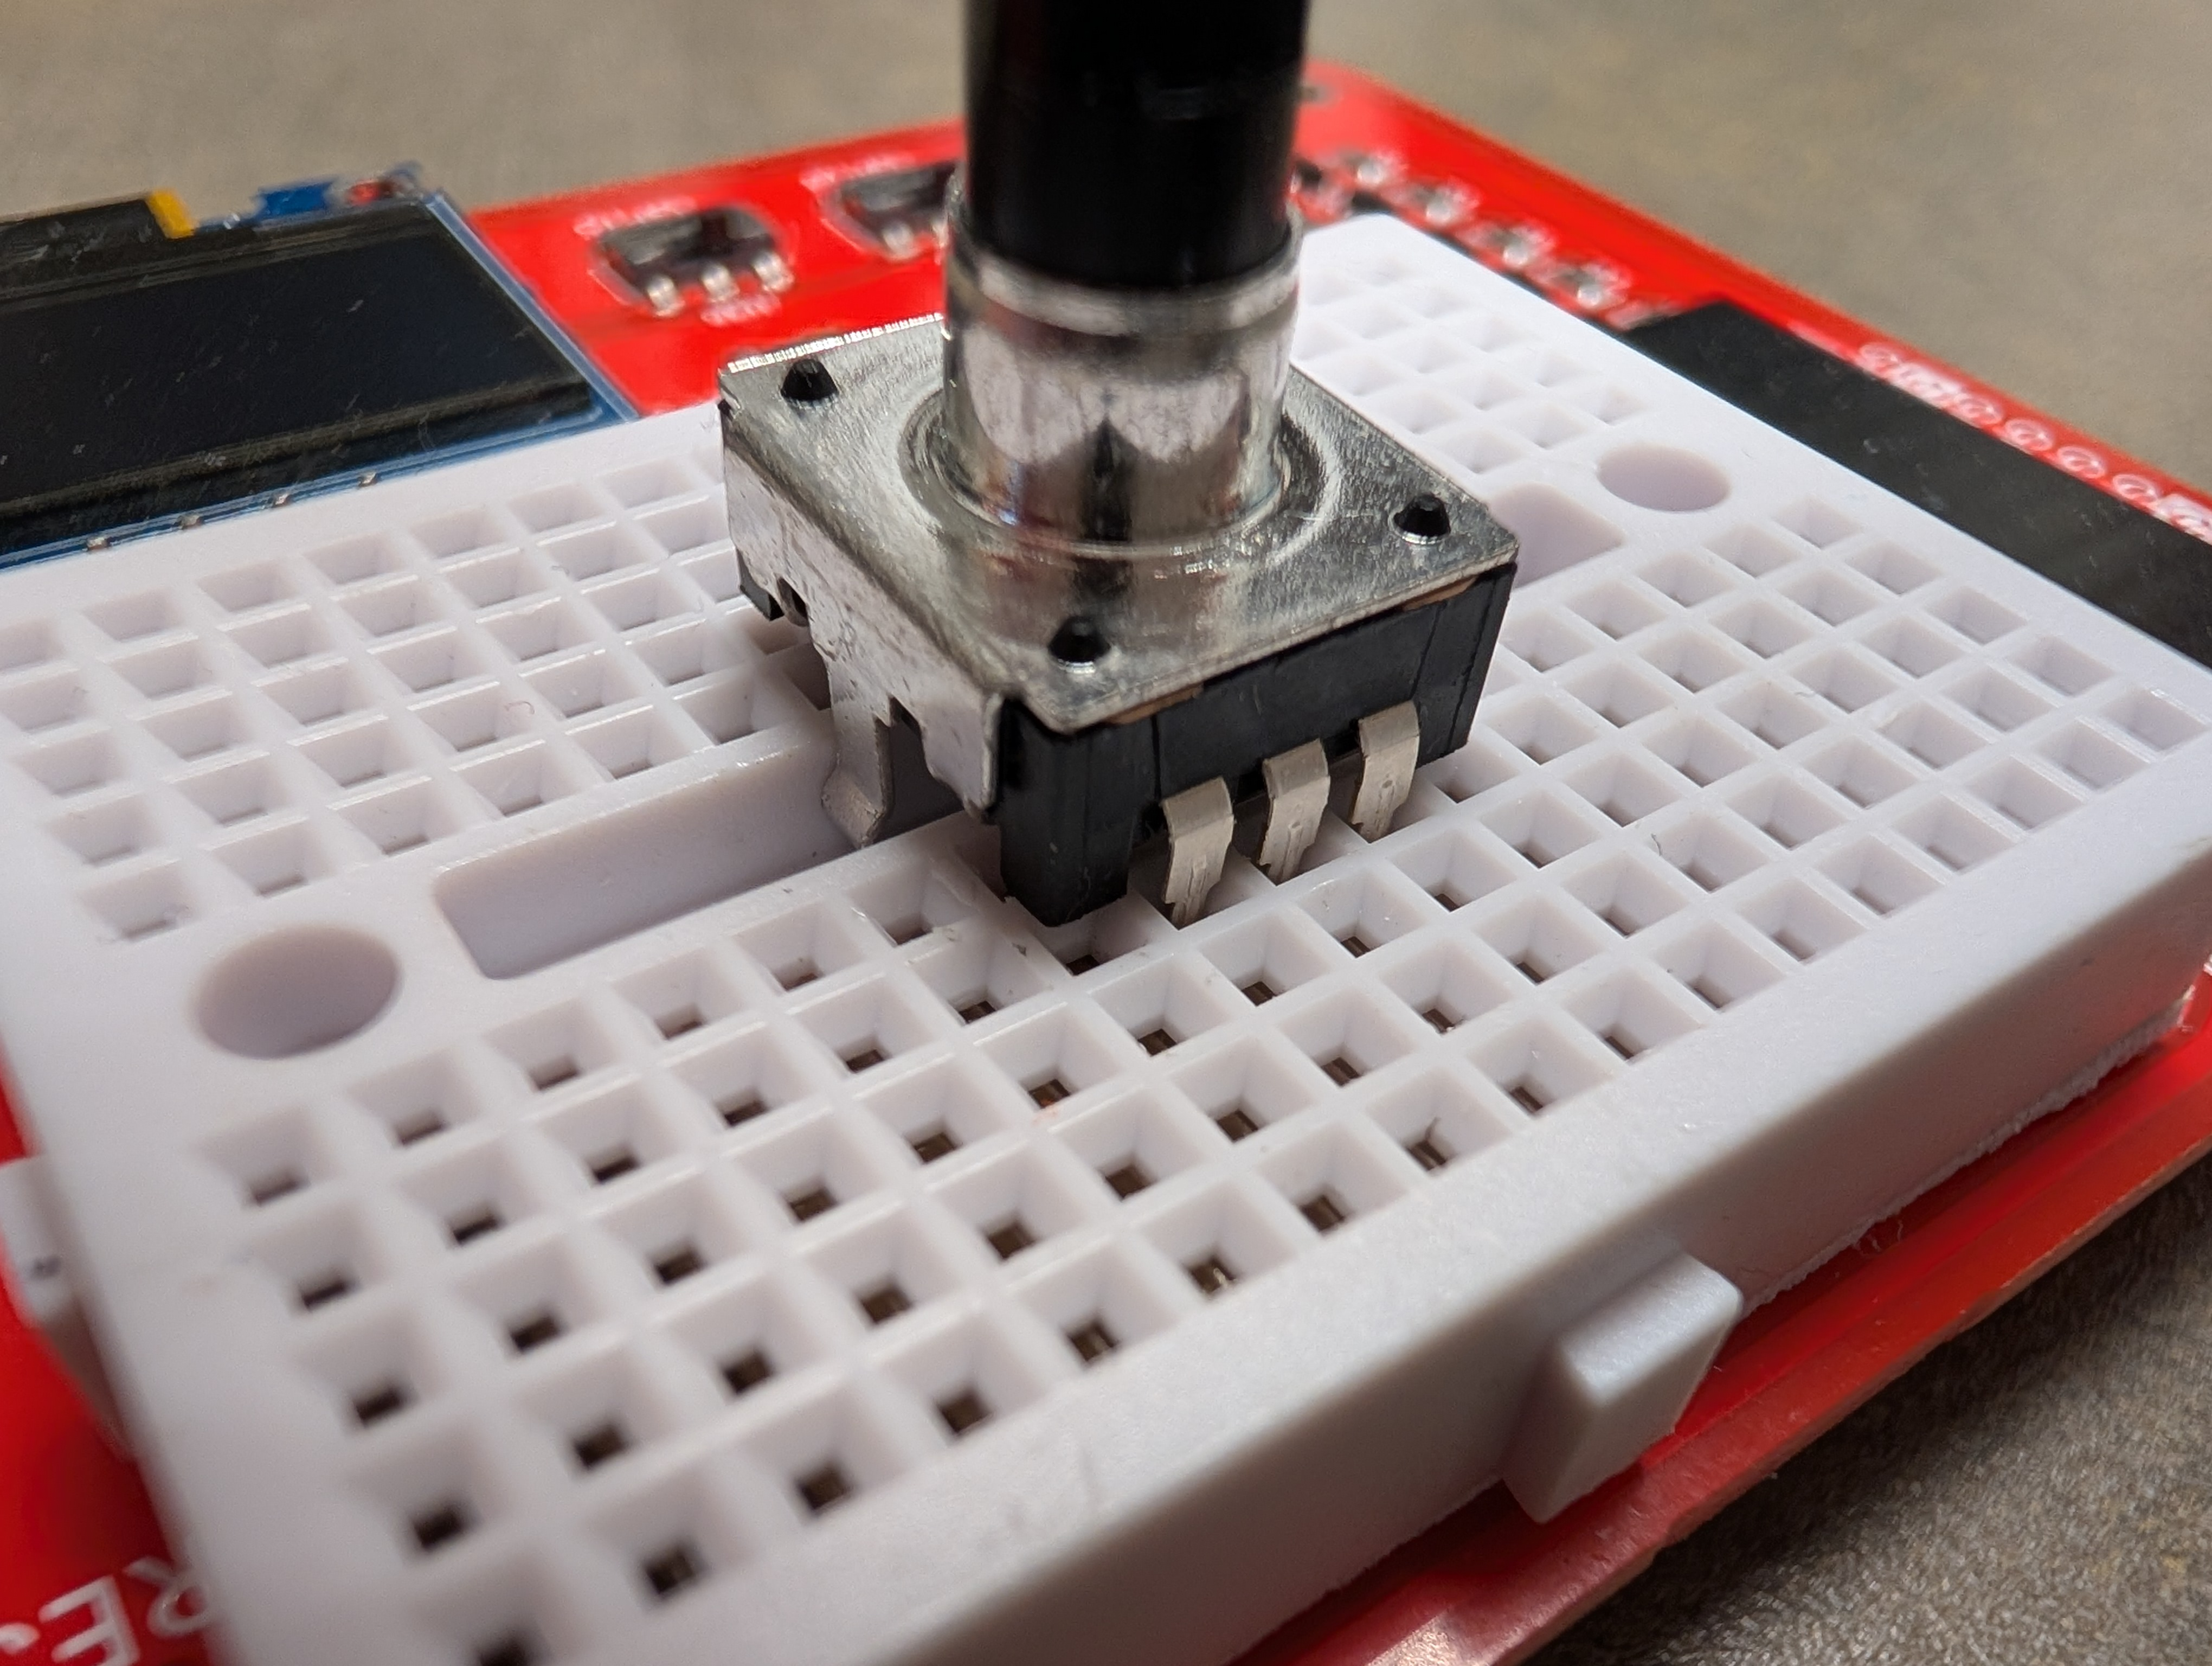
\includegraphics[height=4cm]{hardware/rotaryEncoderInserted}
        \label{fig:rotaryEncoderInserted}
    }
    \\
    \subfloat[Lining up the wires.]{
        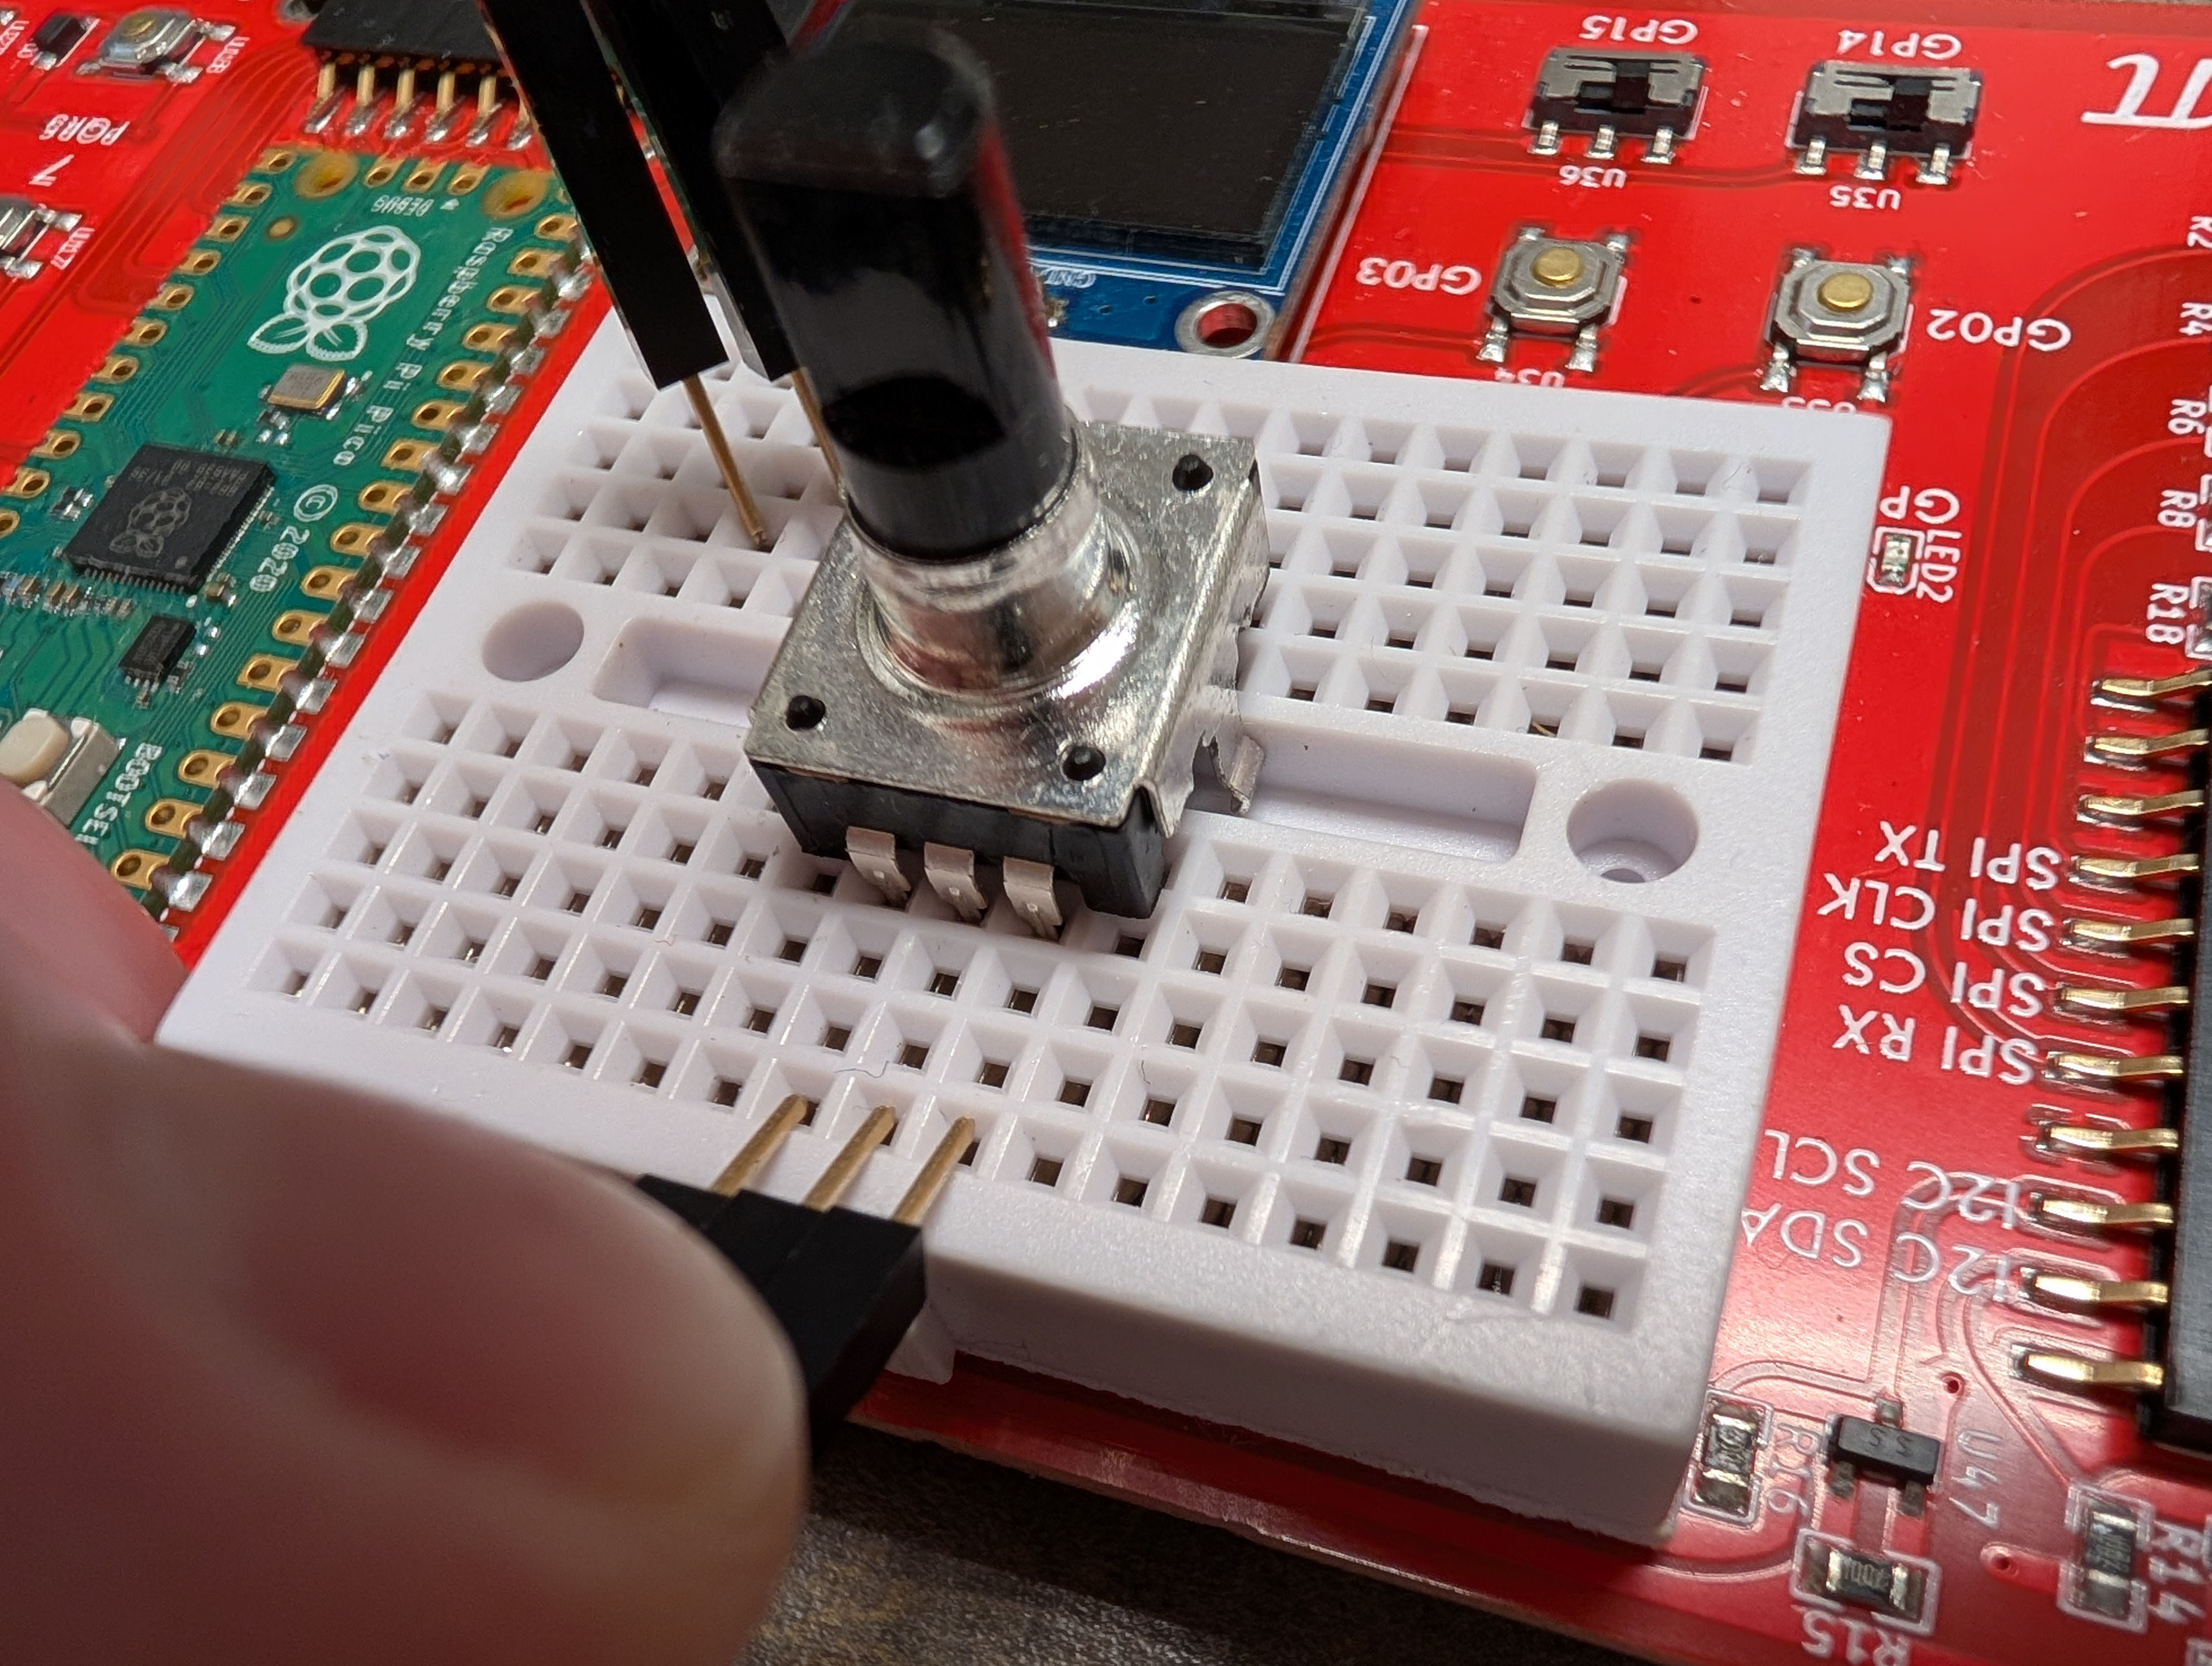
\includegraphics[height=4cm]{hardware/rotaryEncoderAligningWires}
        \label{fig:rotaryEncoderAligningWires}
    }
    \hfil
    \subfloat[Wires connected to the rotary encoder.]{
        \includegraphics[height=4cm]{hardware/rotaryEncoderWiresBreadboard}
        \label{fig:rotaryEncoderWiresBreadboard}
    }
    \caption{Inserting the rotary encoder in the breadboard. \label{fig:rotaryEncoderBreadboard}}
\end{figure}

\begin{description}
    \checkoffitem{Position the rotary encoder on the breadboard so that the prongs on either side of the encoder will fit in the breadboard's gutter (Figure~\ref{fig:rotaryEncoderProngs}),
        and with the three pins positioned in the wells of three contact points (Figure~\ref{fig:rotaryEncoderPins}).}
    \checkoffitem{Gently but firmly, press on the rotary encoder until the bottom of the encoder is flush with the top of the breadboard (Figure~\ref{fig:rotaryEncoderInserted}).}
    \checkoffitem{Insert three 20cm wires, one into each of the same terminal strips that the rotary encoder uses (Figure~\ref{fig:rotaryEncoderAligningWires}--\ref{fig:rotaryEncoderWiresBreadboard}).
        Make a note of which color wire corresponds to which of the sensor's pins.}
\end{description}

The three pins are connected to the rotary encoder's \texttt{A} and \texttt{B} wipers, and to a \texttt{C}ommon ground.
See Figure~\ref{fig:rotaryEncoderLabels} for a labeling of the pins.

\begin{figure}
    \centering
    \subfloat[Labeled pins]{
        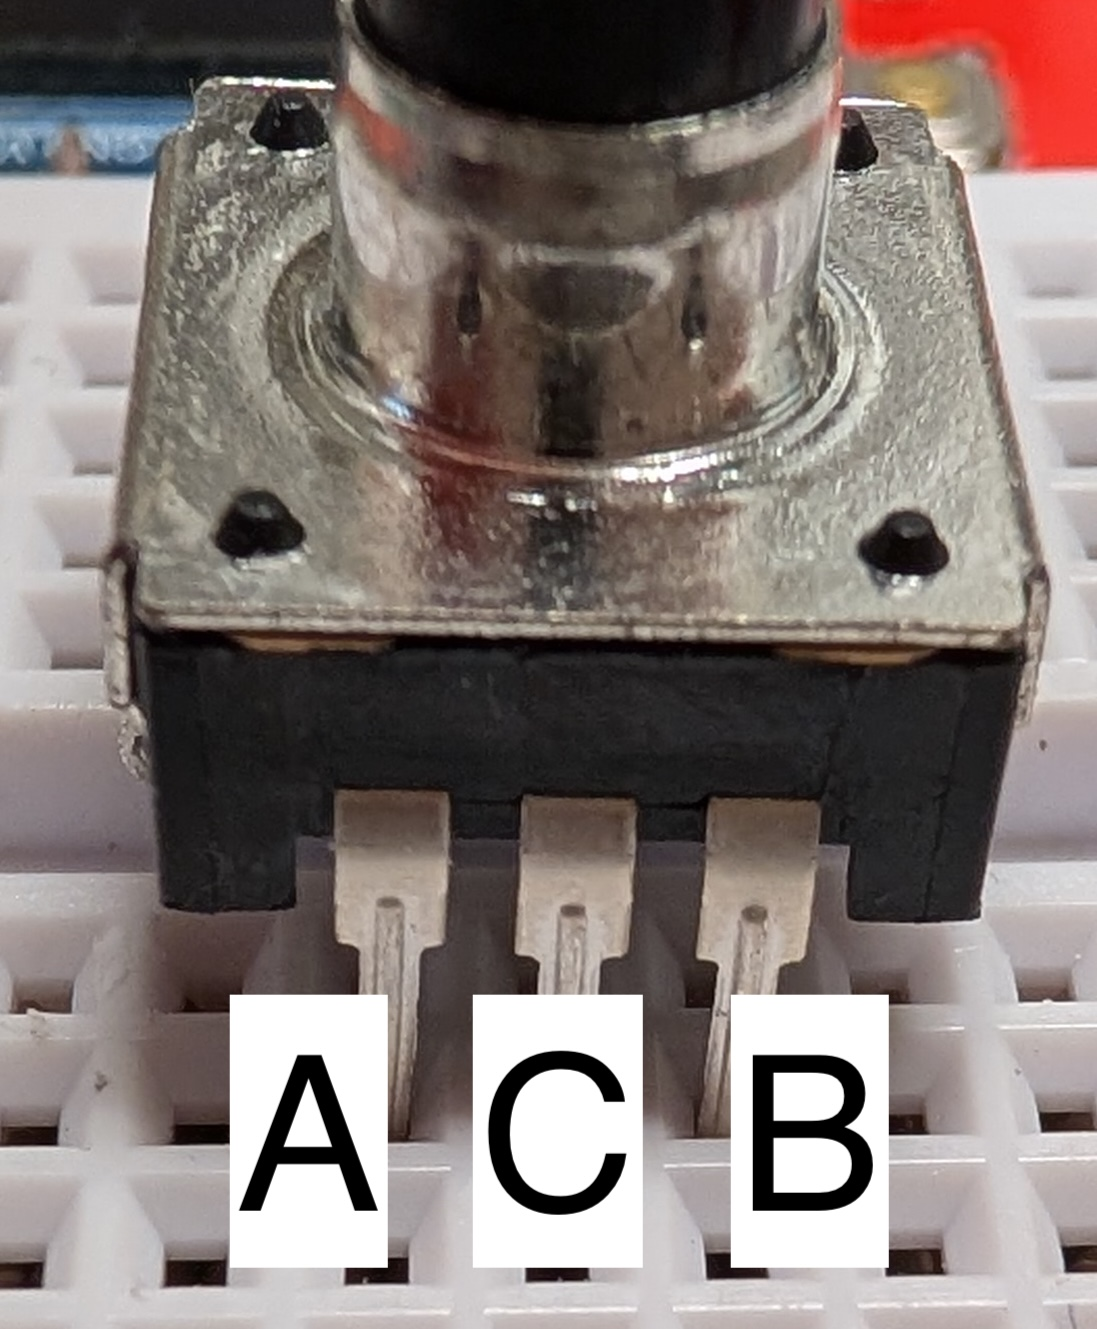
\includegraphics[height=4cm]{hardware/rotaryEncoderPins-labeled}
        \label{fig:rotaryEncoderLabels}
    }
    \hfil
    \subfloat[Inserting the ground wire] {
        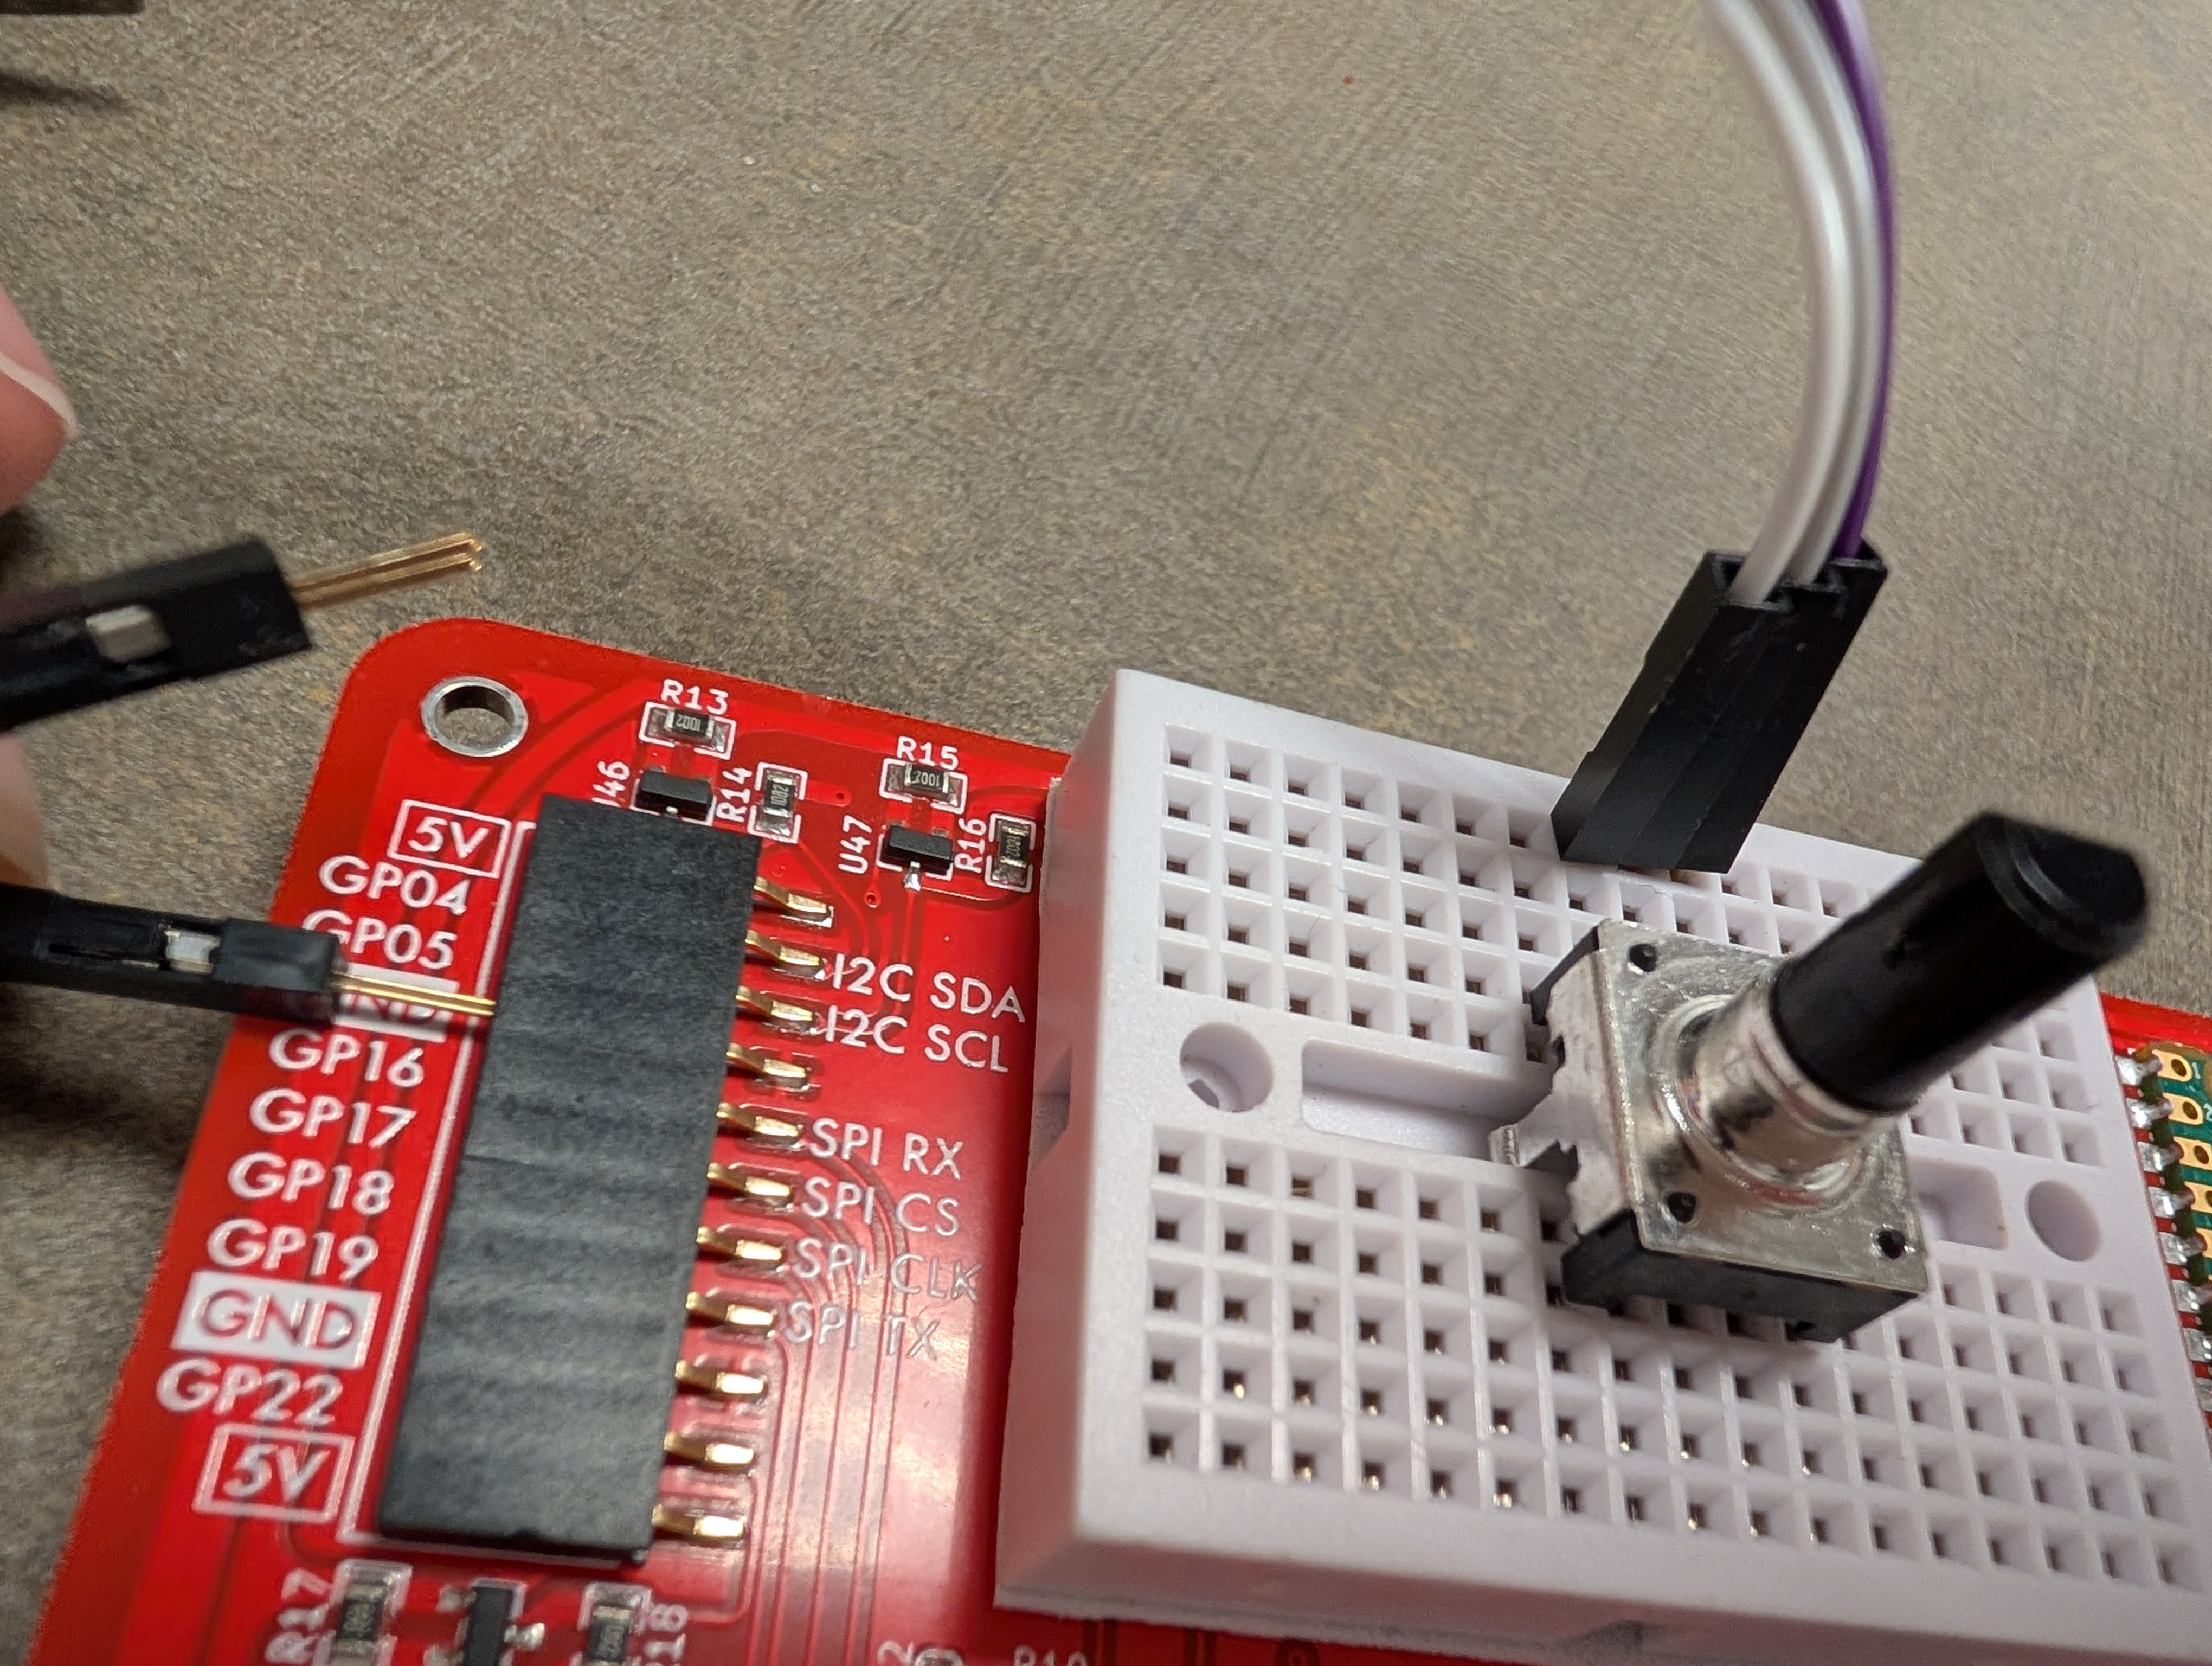
\includegraphics[height=4cm]{hardware/rotaryEncoderGround}
        \label{fig:rotaryEncoderGround}
    }
    \\
    \subfloat[Inserting the A wiper's wire] {
        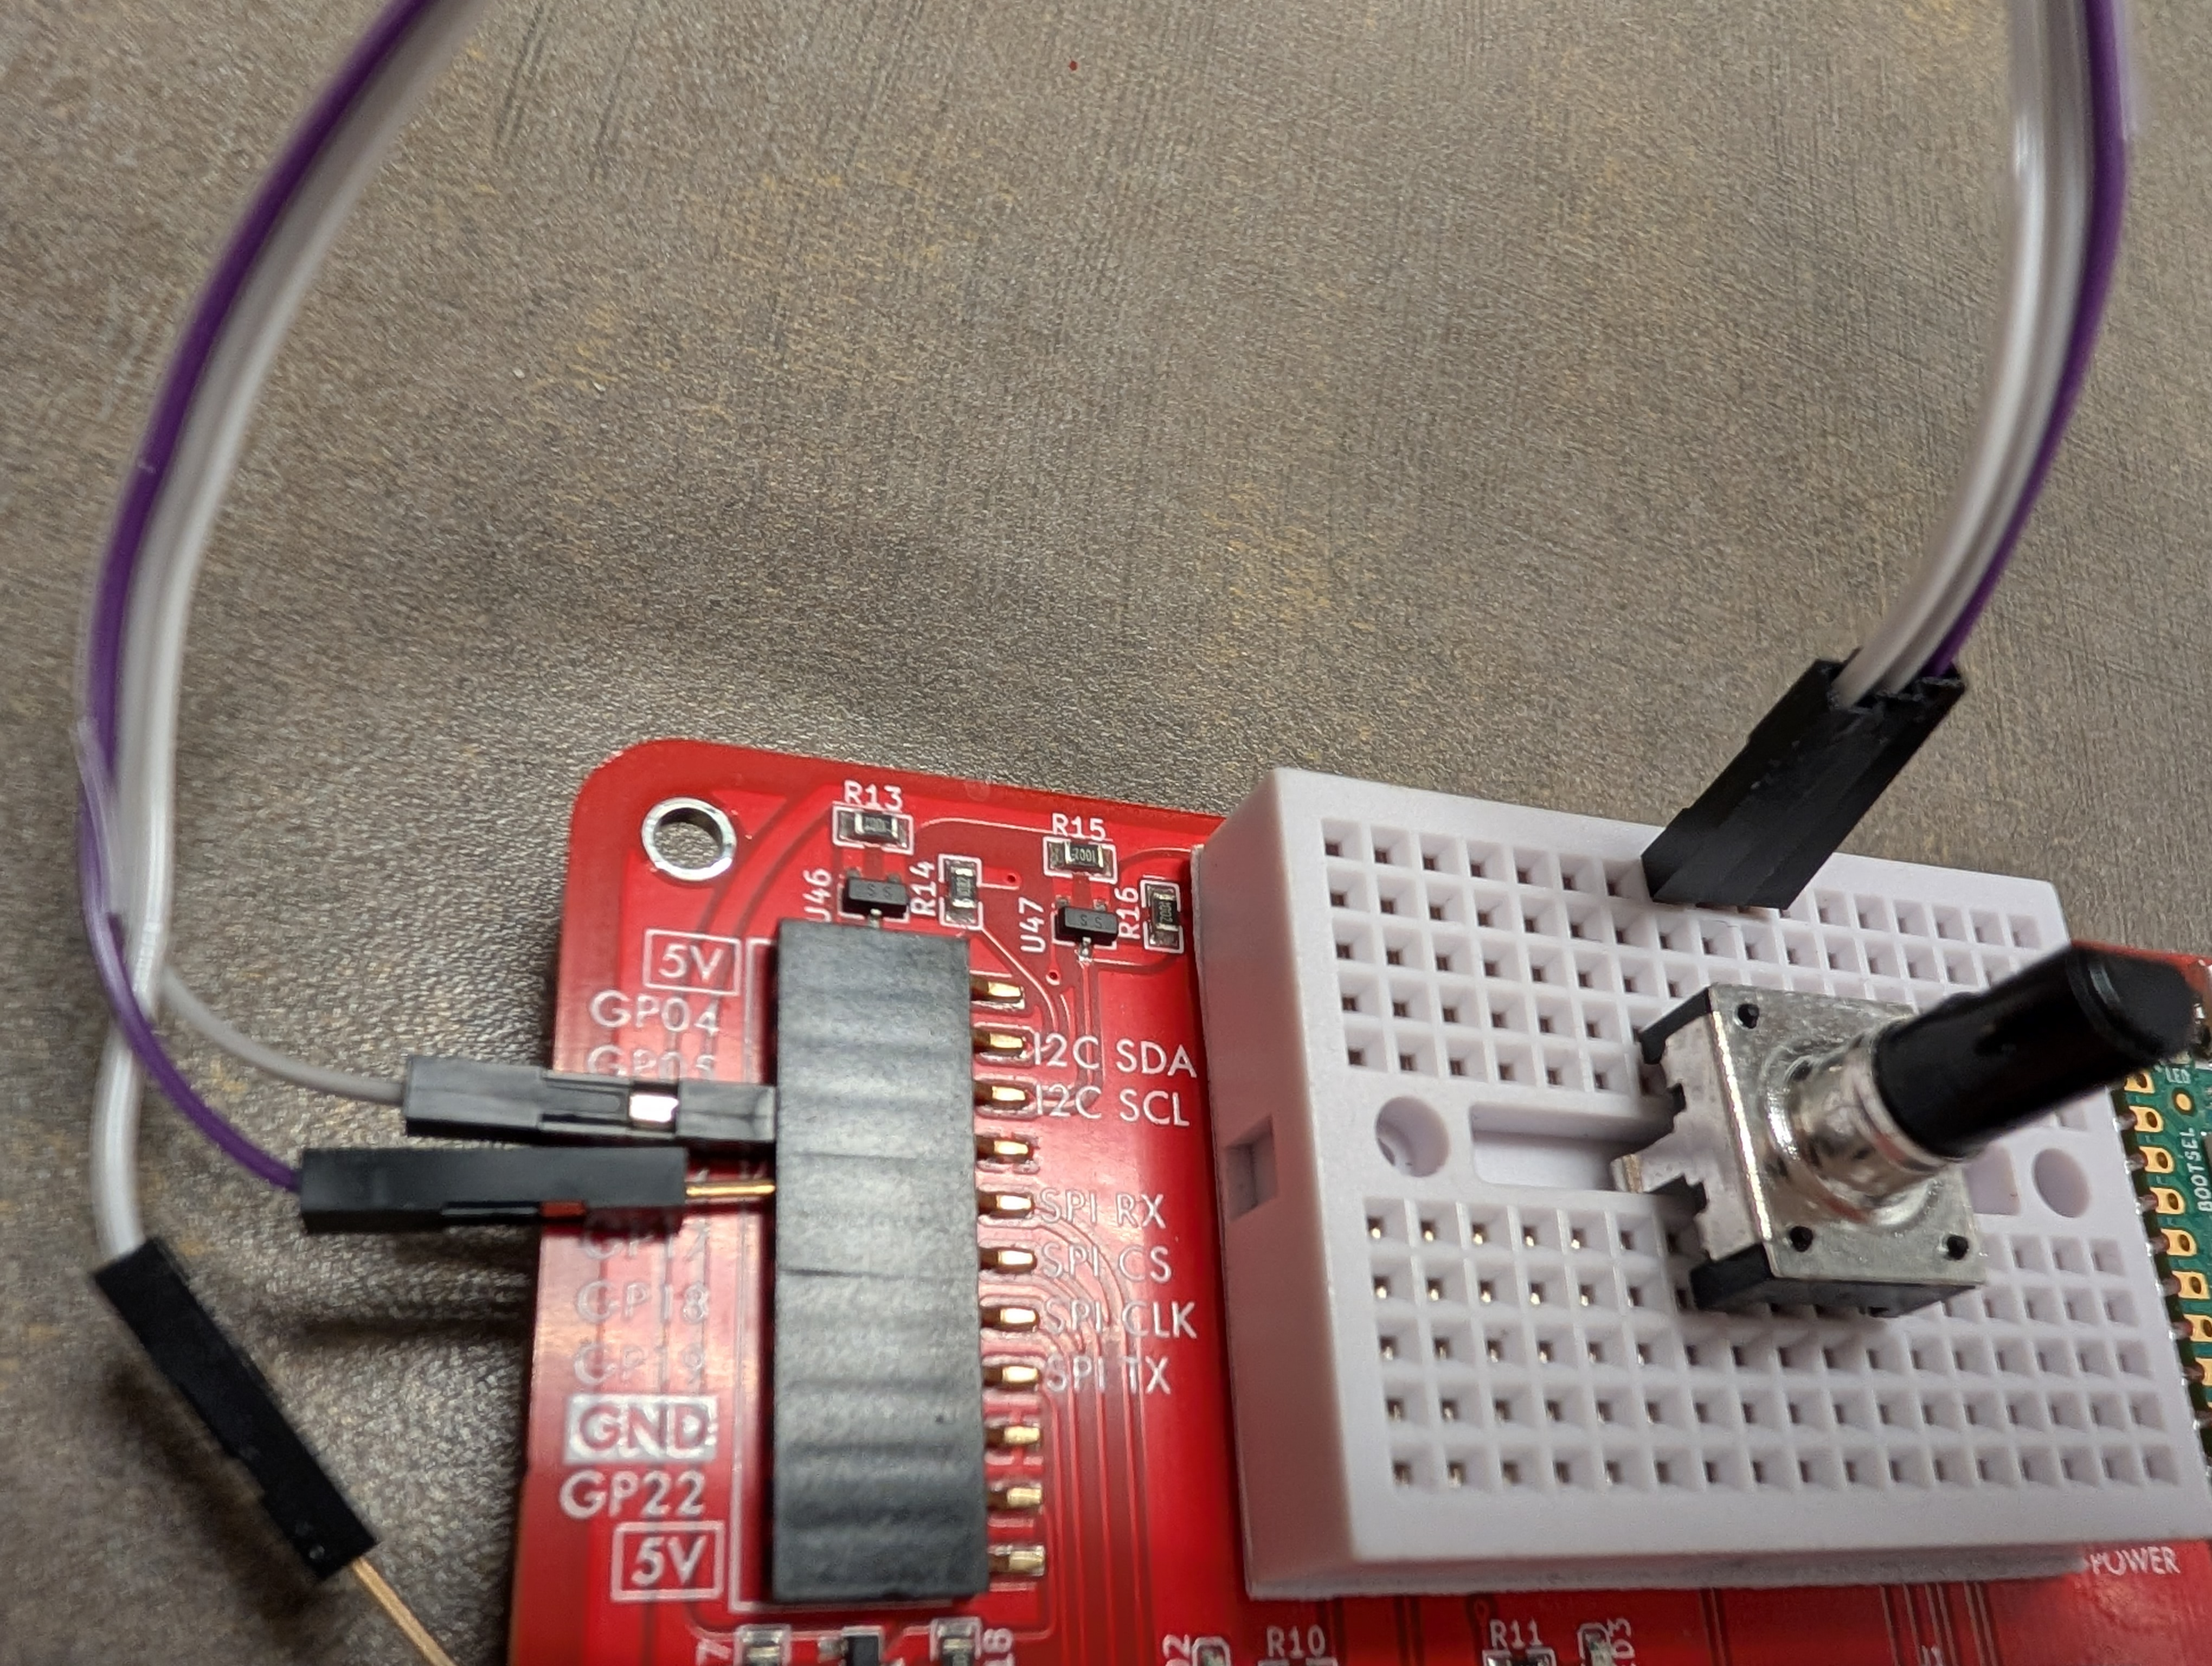
\includegraphics[height=4cm]{hardware/rotaryEncoderApin}
        \label{fig:rotaryEncoderApin}
    }
    \hfil
    \subfloat[Inserting the B wiper's wire] {
        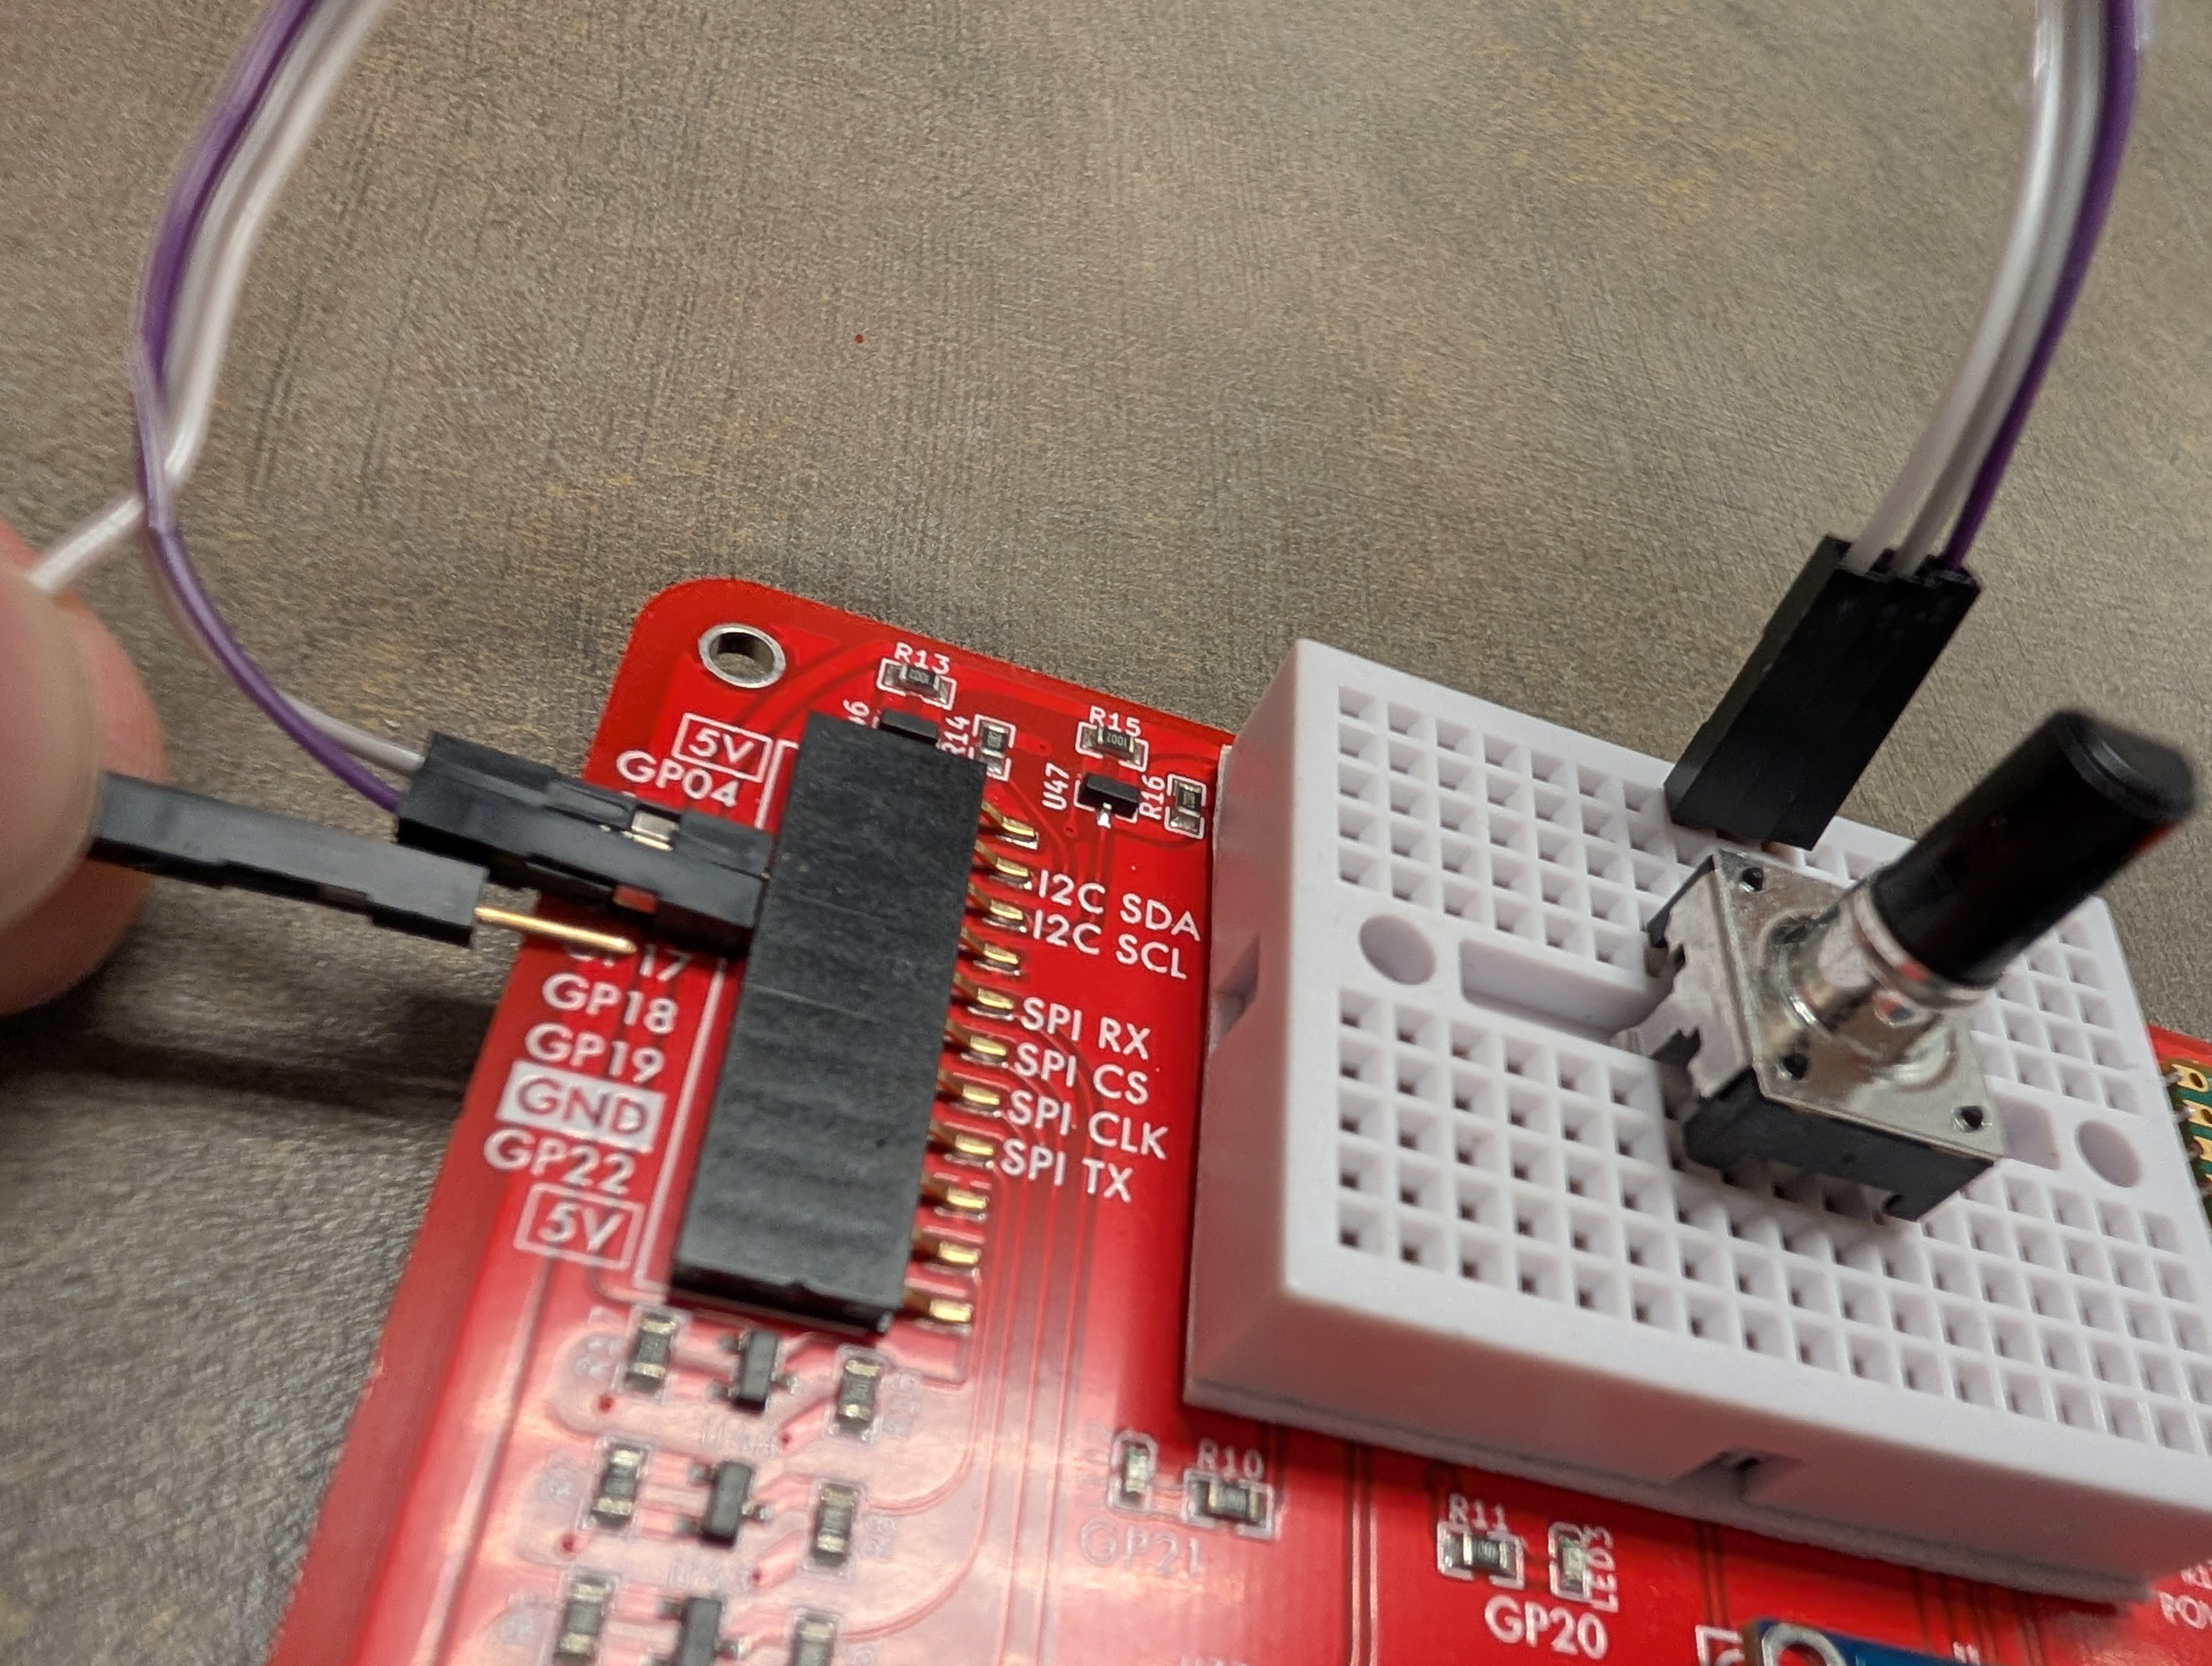
\includegraphics[height=4cm]{hardware/rotaryEncoderBpin}
        \label{fig:rotaryEncoderBpin}
    }
    \caption{Wiring a rotary encoder to the Cow~Pi.}
\end{figure}

\begin{description}
    \checkoffitem{Locate the 20cm that is attached to the rotary encoder's \textbf{\texttt{C}} pin. Insert the other end into a \texttt{GND} slot (Figure~\ref{fig:rotaryEncoderGround}).}
    \checkoffitem{Locate the 20cm that is attached to the rotary encoder's \textbf{\texttt{A}} pin. Insert the other end into the \texttt{GP16} slot.}
    \checkoffitem{Locate the 20cm that is attached to the rotary encoder's \textbf{\texttt{B}} pin. Insert the other end into the \texttt{GP17} slot.}
    \checkoffitem{\textcolor{red}{Have someone verify that you have each wire inserted into the correct slot.}}
\end{description}

The rotary encoder's quadrature can now be read through the Raspberry Pi Pico's pins \texttt{GP16}--\texttt{GP17}.
The starter code will configure \texttt{GP16} \& \texttt{GP17} to be pulled-up input pins.


\vspace{1cm}

Your Cow~Pi is now ready for you to design and code the software for an electronic combination lock.

\begin{figure}[h]
    \centering
    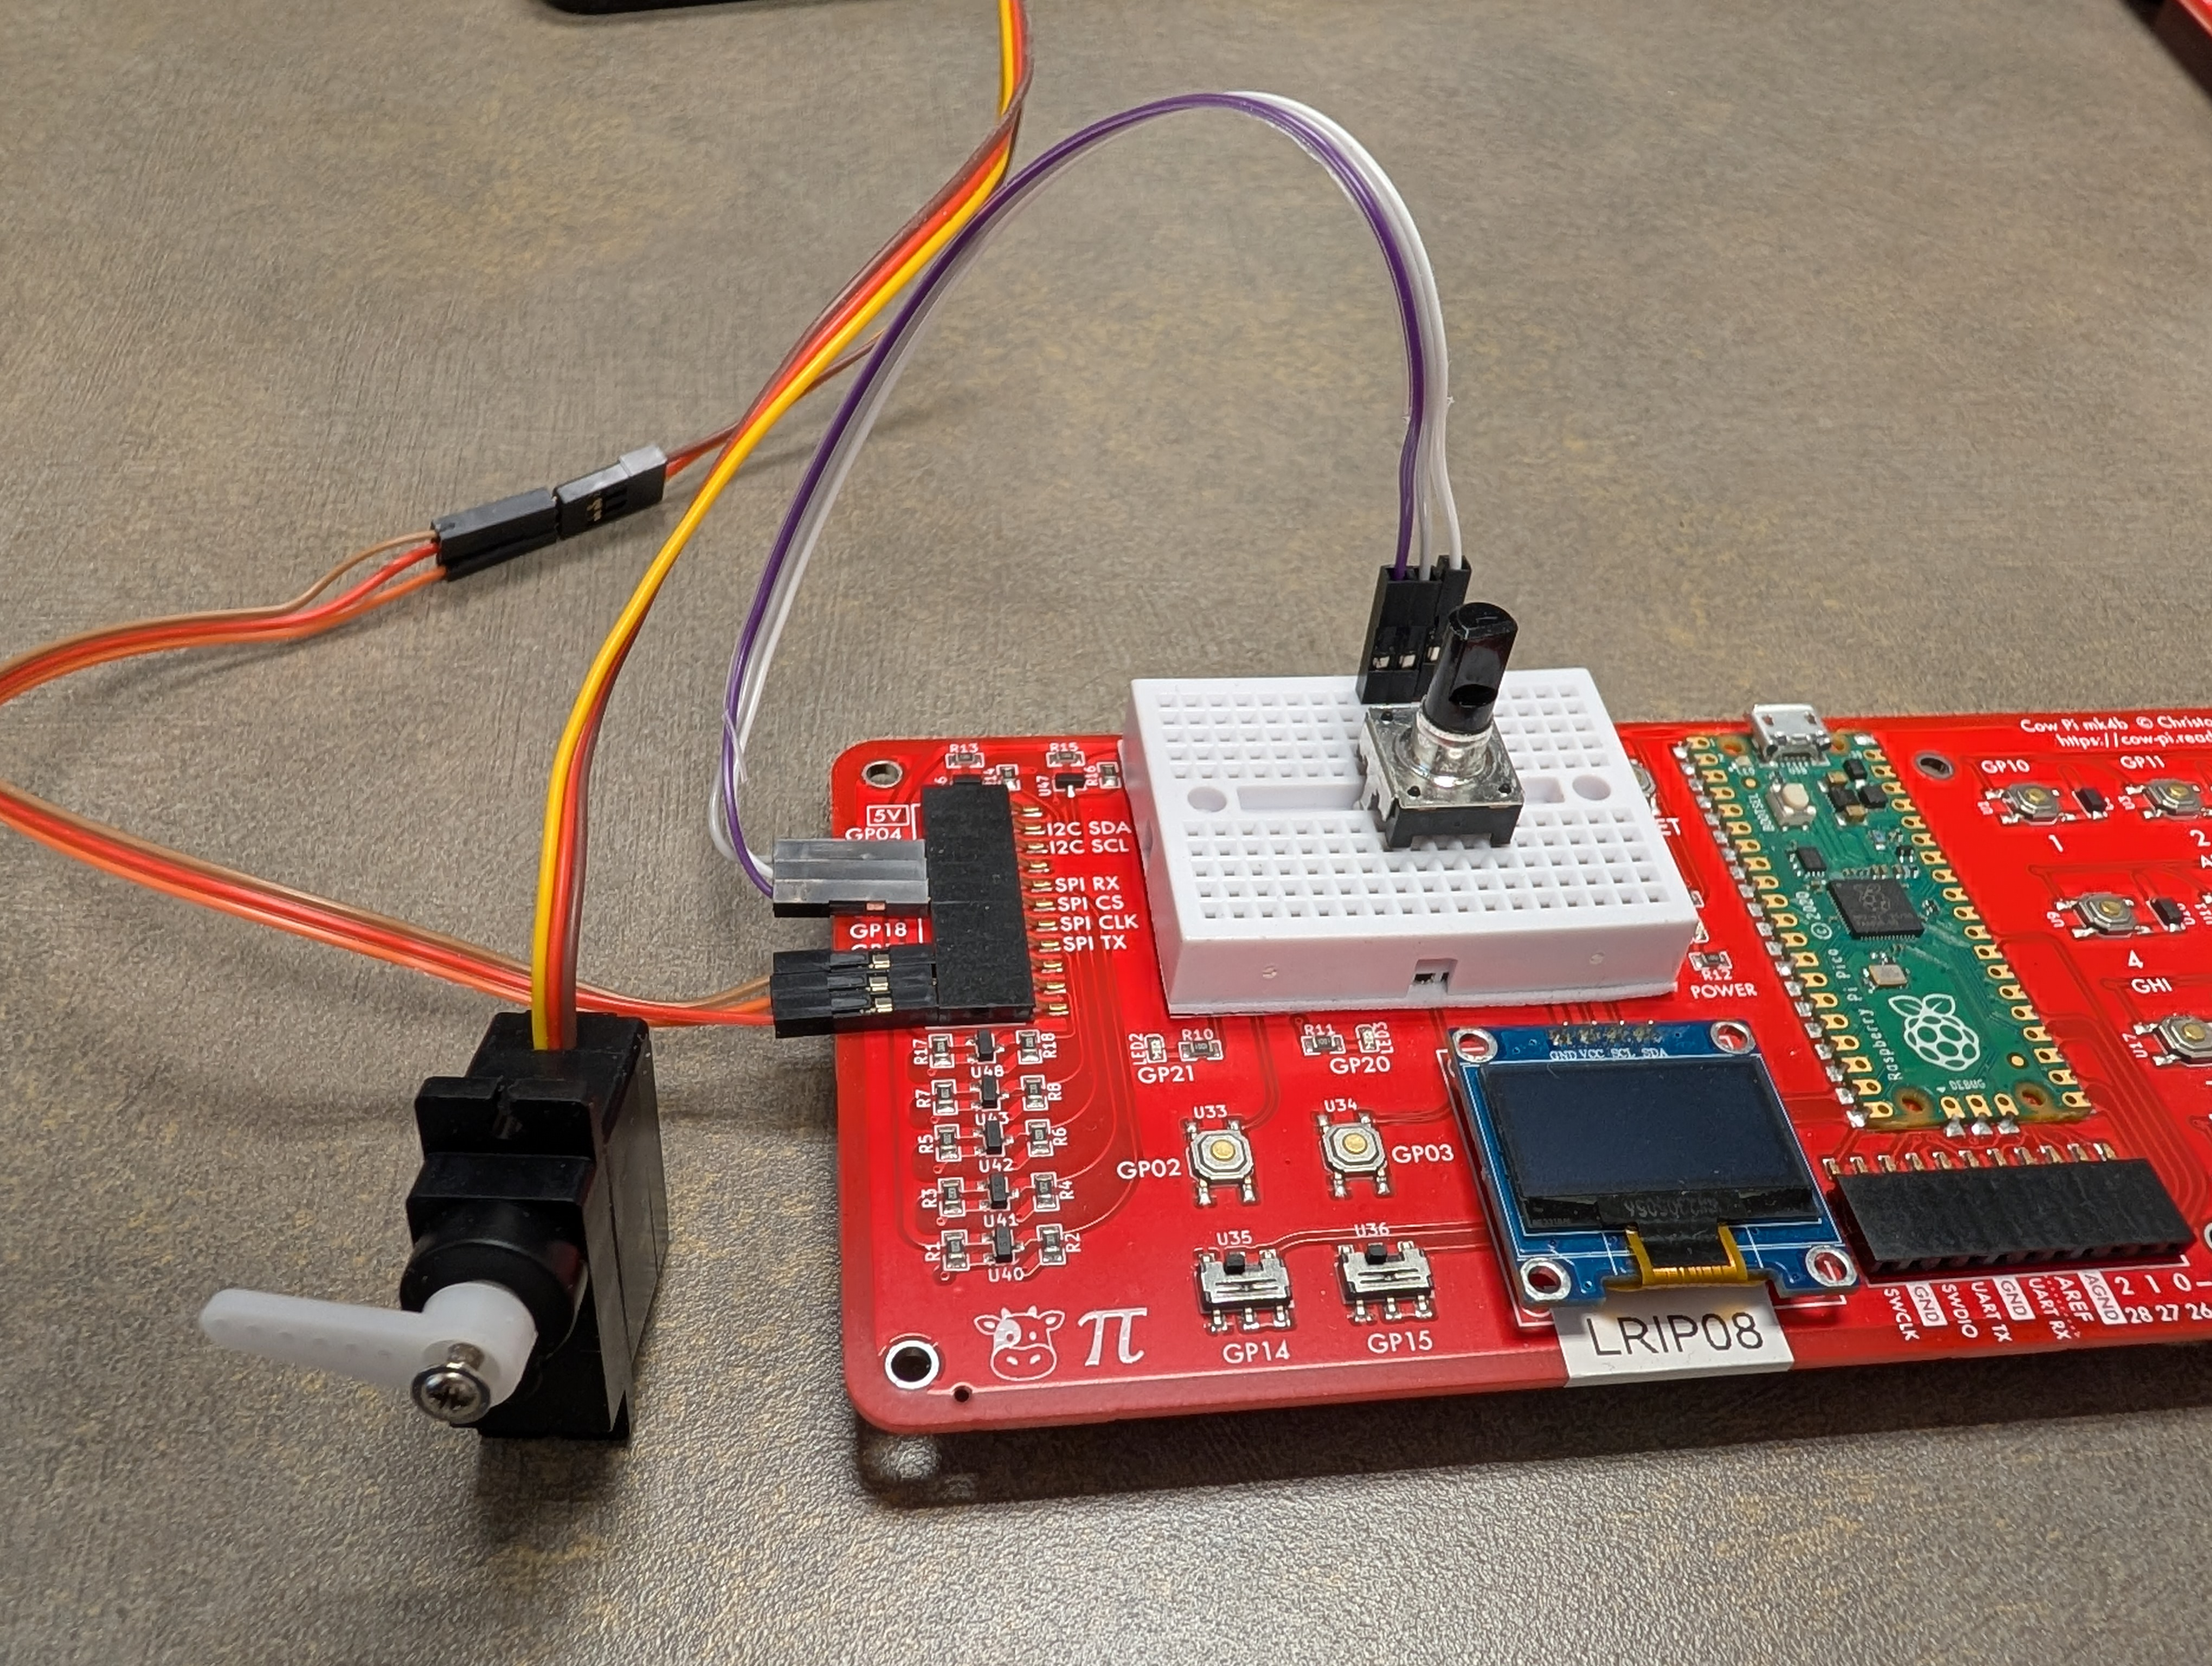
\includegraphics[height=8cm]{hardware/combolock}
    \caption{A fully-assembled combination lock.}
\end{figure}


\end{document}
